\documentclass{report}
\usepackage[utf8]{inputenc}
\usepackage{natbib}
\usepackage{graphicx}
\usepackage{wrapfig}
\usepackage{subfig}
\usepackage{floatrow}
\usepackage[dutch]{babel}
\usepackage{pdfpages}
\PassOptionsToPackage{hyphens}{url}\usepackage{hyperref}
\floatsetup[table]{capposition=top}

\usepackage{afterpage}

\newcommand\blankpage{%
    \null
    \thispagestyle{empty}%
    \addtocounter{page}{-1}%
    \newpage}
    
    \usepackage{mathptmx}
\usepackage[11pt]{moresize}

\usepackage[acronym,footnote,nonumberlist]{glossaries} 
\usepackage{glossary-mcols}
\include{Glossary}
\makeglossaries
\glossarystyle{mcolindex}

\renewcommand*\contentsname{Inhoudsopgave}
\renewcommand{\listfigurename}{Figurenlijst}
\renewcommand{\listtablename}{Tabellenlijst}

\setlength\parindent{0pt}
\begin{document}
\pagenumbering{roman}


\includepdf[page=-]{voorblad/titel} 
\afterpage{\blankpage}

\chapter*{Preambule}
Ten gevolge van de coronamaatregelen gedurende de periode waarin deze thesis werd uitgewerkt, werden enkele hindernissen ondervonden. Het was onmogelijk om in fysiek contact te komen met voldoende proefpersonen. Pogingen om dit op afstand te volbrengen zijn niet geslaagd omwille van een te kort aan benodigd materiaal. De proefpersonen zouden namelijk moeten beschikken over een functionerend springtouw en een smartwatch. Bijgevolg werd deze studie volbracht met slechts een 4-tal proefpersonen.

\chapter*{Dankwoord}
Deze thesis kon niet tot volbracht worden zonder de hulp en steun van een aantal personen. Graag bedank ik mijn begeleiders prof. dr. ir. Toon De Pessemier en prof. dr. ir. Luc Martens omwille van de goede begeleiding en het steeds beantwoorden van mijn vele vragen.
Dit onderzoek kan niet tot een goed einde gebracht worden zonder de inzet van de proefpersonen. Vandaar bedank ik Tim Steels, Diana de Croocq en Annick Audenaert. Zij hebben de verschillende bewegingen talloze keren uitgevoerd zonder te klagen. Hierbij bedank ik Tim Steels eveneens voor de mentale steun gedurende het onderzoek.
Als laatste bedank ik Marleen Denert voor de goede coördinatie en opvolging van de verschillende masterproeven.
\textbf{\Huge Ontwerp en ontwikkeling van een gezondheidsaanbevelingssysteem gericht op rope skipping} \\

Promotoren: prof. dr. ir. Toon De Pessemier, prof. dr. ir. Luc Martens \\
Masterproef ingediend tot het behalen van de academische graad van Master of Science in de industriële wetenschappen: informatica \\
Academiejaar 2019-2020
\\\\
\textbf{\LARGE Abstract} \\\\
Fysieke activiteit is broodnodig in onze sedentaire samenleving. Zonder enige vorm van persoonlijke coaching is dit echter niet efficiënt te realiseren. Tegenwoordig heeft iedereen wel een soort mobiel toestel op zak. Dit is een bron van mogelijkheden op vlak van fysieke activiteit coaching. Een smartwatch geeft hier nog een extra dimensie aan door de fysieke activiteit rechtstreeks te monitoren op basis van hartslagsensoren. Deze data maakt het mogelijk om ook persoonlijke aanbevelingen te produceren.
Één van de meest gebruikte argumenten in het voordeel van te weinig beweging is het gebrek aan tijd. Hiervoor is \textit{rope skipping} de ideale oplossing. Deze sport zorgt namelijk voor optimale conditietraining waardoor gebruikers efficiënt bewegen. Ook kan deze sport eender waar uitgeoefend worden mits enige plaats. Qua bewegingsherkenning van specifieke rope skipping bewegingen werd nog bitter weinig onderzoek uitgevoerd. Door de bewegingen te herkennen en eventuele tekortkomingen te detecteren, kan echter voor extra aanmoediging gezorgd worden.
Deze paper beschrijft een android applicatie ontwikkeld om de gebruiker een gezond bewegingspatroon aan te leren met toevoeging van het extra element rope skipping. 
In een eerste deel wordt bestaande literatuur bekeken met betrekking tot bewegingsherkenning, bepalen van inspanningsniveaus, doel voorspelling en aanbevelingssystemen.
Een tweede deel gaat dieper in op de gebruikte technologieën. Een goed inzicht in het materiaal/de technologieën waarmee gewerkt wordt is namelijk vereist. 
Vervolgens wordt meer verteld over het bewegingsherkenning proces. Door verzameling van data afkomstig van verschillende proefpersonen wordt een model ontwikkeld. Dit model is in staat om vijf rope skipping bewegingen te classificeren.
In een laatste deel wordt de gezondheidsapplicatie toegelicht. Deze applicatie gaat, gebaseerd op het inspanningsniveau bij de verschillende rope skipping bewegingen, aanbevelingen genereren. Het inspanningsniveau wordt bepaald aan de hand van de MET metriek. Het aantal METs is afhankelijk van de tijd die in een bepaalde hartslag zone doorgebracht werd. Aanbevelingen worden berekend aan de hand van enerzijds de frequentie van uitvoering en het gemiddeld aantal METs verbruikt per minuut per beweging, anderzijds de hoeveelheid gemaakte fouten. Door te werken met een doel wordt een bovengrens gecreëerd voor het aantal aanbevelingen. Dit doel wordt bepaald door historische data tot 10 weken in het verleden te bekijken en hier het gemiddelde van te nemen.\\\\

\noindent
\textbf{Trefwoorden: rope skipping, gezondheidsapplicatie, wear OS, android, recommender system, machine learning, neuraal netwerk}



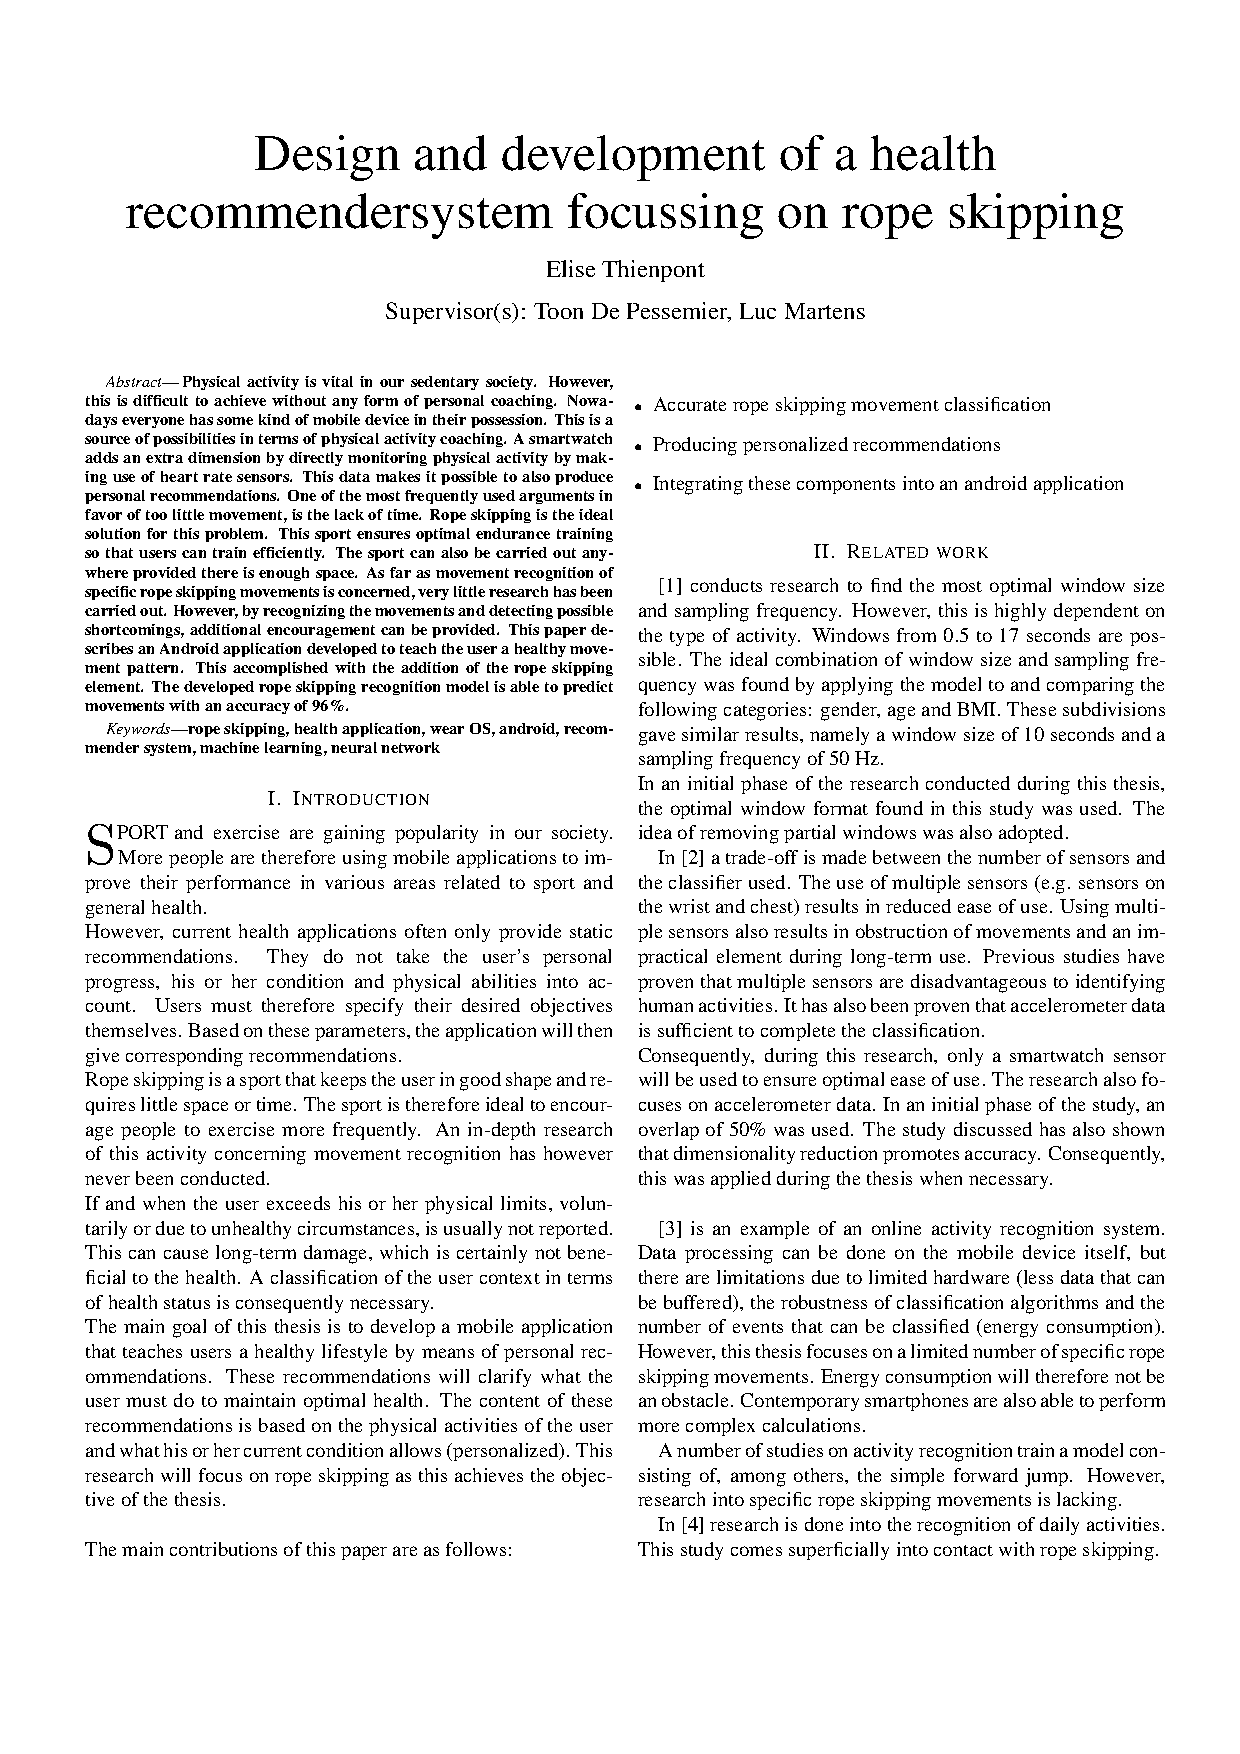
\includepdf[page=- ,  pagecommand={\thispagestyle{plain}}, scale=0.9]{voorblad/extended_abstract} 

\tableofcontents
\newpage

\listoffigures
\newpage

\listoftables
\newpage

\chapter*{Lijst van afkortingen}

\newcommand{\abbrlabel}[1]{\makebox[3cm][l]{\textbf{#1}\ }}
\newenvironment{abbreviations}{\begin{list}{}{\renewcommand{\makelabel}{\abbrlabel}}}{\end{list}}
\begin{abbreviations}
\item[MAXHR] Maximale hartslag
\item[MET] Metabolic equivalent of task
\item[RMR] Resting metabolic rate
\item[SED] Sedentary
\item[LPA] Light physical activity
\item[MPA] Moderate physical activity
\item[VPA] Vigourous physical activity
\item[SMV] Signal magnitude vector
\item[SMA] Signal magnitude area
\item[PSD] Power spectral density
\item[CNN] Convolutional neural network
\item[SVM] Support vector machine
\item[SVC] Support vector classification
\item[SGD] Stochastic gradient descent
\item[MLP] Multilayer perceptron 

\end{abbreviations}

\pagenumbering{arabic}

\chapter*{Introductie}

\section*{Probleemstelling}
Sport en beweging wint steeds aan populariteit in onze samenleving. Meer mensen gebruiken dan ook mobiele applicaties om hun sportprestaties en algemene gezondheid te verbeteren.  

Huidige gezondheidsapplicaties geven echter vaak enkel statische aanbevelingen. Ze houden geen rekening met de persoonlijke vooruitgang van de gebruiker, zijn of haar conditie en fysieke capaciteiten.  Gebruikers moeten zelf hun gewenste doelstellingen opgeven. De applicatie zal dan, gebaseerd op deze parameters, bijhorende aanbevelingen geven. 

Rope skipping is een sport die voor een goede conditie zorgt en weinig plaats of tijd vergt. De sport is dus uitermate geschikt om mensen aan te zetten tot meer beweging. Een diepgaande opvolging van deze activiteit werd nog niet eerder op punt gezet.
 
Indien de gebruiker zijn/haar fysieke grenzen overschrijdt, omwille van vrijwillige forcering of ongezonde omstandigheden, wordt dit meestal niet gemeld. Hierdoor kunnen langdurige klachten ontstaan, wat de gezondheid zeker niet ten goede komt. Een classificatie van de gebruikerscontext in termen van gezondheidstoestand is noodzakelijk. 
 
\section*{Doelstelling}
Het doel van deze thesis is het ontwikkelen van een mobiele applicatie die gebruikers een gezonde levensstijl aanleert door persoonlijke aanbevelingen te produceren. Deze aanbevelingen zullen duidelijk maken wat de gebruiker moet doen om in optimale gezondheid te blijven. De inhoud hiervan is gebaseerd op de fysieke activiteiten van de gebruiker en wat zijn/haar huidige conditie toelaat (gepersonaliseerd). Dit onderzoek zal zich focussen op rope skipping aangezien dit de doelstelling van de thesis goed verwezenlijkt. 
 
De thesis zal een antwoord bieden op volgende onderzoeksvraag: “Hoe kan vanuit ruwe data (hartslag, beweging) een gepersonaliseerd bewegingspatroon ontwikkeld worden?” 

Het probleem van statische, niet gepersonaliseerde aanbevelingen wordt aangepakt door een op maat gemaakt bewegingspatroon te creëren voor iedere gebruiker. Via algoritmen die ruwe data van sensoren (hartslag, beweging) omzetten in specifieke activiteiten of inspanningsniveaus zal dit ontwikkeld worden.  
 
Ook zal er aandacht besteed worden aan bepaalde deelonderzoeksvragen. Een eerste van deze deelonderzoeksvragen luidt als volgt: “Is het mogelijk om specifieke rope skipping bewegingen te herkennen op basis van accelerometer data?". Aangezien accelerometer een zeer energiezuinige sensor is, focust deze thesis zich hoofdzakelijk op deze data. Via bewegingsherkenning kan gedetecteerd worden welke activiteiten de gebruiker verkiest. Hierdoor wordt het systeem persoonlijker. Ook zal door middel van foutdetectie een aanmoedigingsmechanisme ontwikkeld worden. 
 
Een tweede deelonderzoeksvraag omvat: “Wanneer wordt intensief bewegen ongezond?” Een classificatie van de gebruikerscontext in termen van gezondheidstoestand kan bekomen worden door constante monitoring van de hartslag. Via deze data kunnen ongewone patronen gedetecteerd worden. Hieruit kan afgeleid worden of de fysieke toestand van de gebruiker verdere intensieve beweging toelaat. 
 
 


\chapter{Literatuurstudie}
\section{Bewegingsherkenning}
Een eerste luik van de literatuurstudie verdiept zich in de verschillende technieken omtrent \textit{activity recognition}. Dit is van groot belang in het kader van rope skipping als middel voor conditietraining.
Op vlak van bewegingsherkenning werd reeds omvangrijk onderzoek verricht. In wat volgt worden relevante studies meer in detail besproken. \\

\subsection{Algemeen}

In \citep{ref1} probeert men aan de hand van \textit{deep learning} een accurater bewegingsherkenning model te creëren.

Gebruik maken van deep learning methoden heeft namelijk vele voordelen in termen van systeem performantie en flexibiliteit. oppervlakkige modellen blijven vaak hangen in lokale optima.
Ook is handmatige \textit{feature extraction} hierbij niet meer noodzakelijk. Handgemaakte features zoals statistische berekeningen zijn specifiek voor het probleem en ze kunnen niet veralgemeend worden naar andere domeinen. Menselijke interventie voor selecteren van de meest effectieve features is noodzakelijk bij deze aanpak. 
Een oplossing voor deze problemen vindt men in deep learning. Methodieken op basis van data zoals deep learning kunnen onderscheidende features leren vanuit historische informatie, dit is automatisch en systematisch. Ook zijn deze modellen beter bestand tegen \textit{overfitting}.

Het deep learning model ontwikkeld in dit onderzoek leert de gewichten van het neuraal netwerk en de informatieve features uit onbewerkte data. Het model bestaat uit twee stappen: een \textit{unsupervised, pre training} stap en een \textit{supervised, fine-tuning} stap. De pre training stap leert features aan de hand van \textit{deep belief networks} en \textit{restricted boltzmann machines}.

Data verzameling en training van het model gebeurt offline en dus niet op een mobiel apparaat. Deze studie maakt tijdens de trainingsfase gebruik van een sliding \textit{window}. Dit om de relatie tussen verschillende datapunten eveneens in beeld te brengen.  Met het gemaakte model wordt vervolgens aan online bewegingsherkenning uitgevoerd. 

Deep learning methoden zijn zeker een goede kandidaat voor het classificatie probleem onderzocht in deze thesis. Bijgevolg zal dit, samen met enkele andere algoritmen, uitgewerkt worden.\\

In \citep{ref6}, een tweede studie van bewegingsherkenning op basis van accelerometer data, werden volgende zaken aangehaald. De onbewerkte time series data werd onderverdeeld in segmenten van tien seconden waarbij per segment verschillende features zijn geïdentificeerd. 6 basis feature types werden gebruikt: het gemiddelde, de standaard deviatie, het gemiddeld absoluut verschil, de gemiddelde resulterende versnelling, de tijd tussen pieken en, als laatste,  \textit{binned distribution}. Op basis van deze types wordt een groot aantal features bekomen per segment.
In deze studie werden J48, \textit{logistic regression} en MLP gebruikt als algoritmen. Dit zijn geen deep learning methodes waardoor handmatige feature extraction inderdaad vereist is.
De studie toont aan dat een ensemble van \textit{classifiers} kan gebruikt worden voor complexe activiteiten herkenning. 
Via een train-test split en \textit{10-Fold cross validation} wordt een test dataset bekomen. 

Het verdelen in segmenten van de onderzochte data is noodzakelijk om contextuele features te bekomen uit het signaal. Bijgevolg werd deze techniek toegepast in het kader van dit onderzoek. Ook zullen, bij bepaalde algoritmen die meer features vereisen, de aangehaalde statistische varianten gebruikt worden als zinvolle aanvulling. \\

In \citep{ref13} wordt onderzocht wat de meest optimale window grootte en sampling frequentie is. Dit is echter zeer afhankelijk van het soort activiteit. Windows van 0.5 tot 17 seconden zijn hierbij mogelijk. Deze studie brengt menselijke reactietijd in rekening. Een minimum sampling frequentie van 32Hz is bijgevolg nodig om correcte data te bekomen.
Windows waarin niet genoeg data aanwezig is om de volledige tijd te vullen, partiële windows, worden verwijderd.
Het aantal data objecten in een window hangt af van de window grootte en sampling frequentie. Men kwam tot deze conclusie na een aantal experimenten met variërende window groottes en sampling frequenties.
246 features werden geëxtraheerd en vervolgens gereduceerd tot een aantal van 32 via correlatie gebasseerde \textit{feature selection}. Deze features komen uit zowel het tijd- en frequentiedomein. 
\textit{Random Forest classifier} geeft goede resultaten op de gebruikte dataset in deze studie. 
De ideale combinatie van window grootte en sampling frequentie werd gevonden door toepassing op en vergelijking van volgende categorieën: geslacht, leeftijd en BMI. Deze onderverdelingen gaven gelijkaardige resultaten, namelijk een window grootte van tien seconden en een sampling frequentie van 50 Hz.

In een eerste fase van het onderzoek uitgevoerd tijdens deze thesis werd de optimale window grootte gevonden in deze studie gebruikt. Het idee om partële windows te verwijderen werd eveneens overgenomen. \\

In \citep{ref15} wordt een afweging gemaakt tussen het aantal sensoren en de gebruikte classifier. Het gebruik van meerdere sensoren (bijvoorbeeld sensoren op de pols en borst) resulteert in vermindering van het gebruiksgemak. Gebruik van meerdere sensoren resulteert namelijk in belemmering van bewegingen en een onpraktisch element bij langdurig gebruik. 
Enkel een accelerometer sensor wordt bijgevolg gebruikt met eliminatie van de gyroscoop sensor. Vroegere studies hebben bewezen dat meerdere sensoren nadelig zijn bij het identificeren van menselijke activiteiten. Er werd eveneens bewezen dat accelerometer data voldoende is om de classificatie tot een goed eind te brengen.
Voor signaal segmentatie wordt gebruik gemaakt van een sliding window met 50\% overlap. In deze studie levert dit goede resultaten. 
Een volgende stap is feature extraction. Hierbij worden features berekend gebruikmakend van het tijd- en frequentiedomein. Hierna wordt een \textit{normality test} uitgevoerd om na te gaan of de bekomen features passen in een normale distributie. Als we dit weten kan bepaald worden of parametrische of niet-parametrische classificatie hulpmiddelen vereist zijn. Volgende drie testen worden gehandhaafd: \textit{shapiro-Wilk, kolmogorov-smirnov en anderson-darling}. Als de features niet in een normale distributie passen zijn niet-parametrische tools beter geschikt.
Via het PCA algoritme wordt dimensionale reductie uitgevoerd. Ook worden de bekomen features genormaliseerd naar een interval van 0 tot 1.
In deze studie werd een vergelijking gemaakt tussen de performantie van de machine learning algoritmes voor en na dimensionale reductie. De gemiddelde accuraatheid ligt hoger bij het toepassen van \textit{dimensionality reduction}.
Ook werd de performantie van algoritmes op tijd- en frequentiedomein gebaseerde features vergeleken. Hieruit wordt geconcludeerd dat het frequentie domein betekenisvollere info geeft.

Bijgevolg zal tijdens dit onderzoek enkel gebruik gemaakt worden van een \textit{smartwatch} sensor om zo te zorgen voor optimaal gebruiksgemak. Er wordt eveneens gefocust op accelerometer data. In een eerste fase van het onderzoek werd een overlap van 50\% gehanteerd. De besproken studie heeft ook aangetoond dat dimensionality reduction de accuraatheid bevorderd. Bijgevolg werd dit toegepast tijdens het onderzoek waar nodig. \\

In \cite{ref76} wordt onder andere een vergelijking gemaakt tussen multi en single sensor gebruik. Hierbij werd geconcludeerd dat gebruik van meerdere sensoren resulteert in een accuraatheid van 94\% tot 96\% terwijl enkele sensoren accuraatheden tussen 90\% en 92\% vertonen. Deze studie focust op activiteiten zoals wandelen, zitten en trantities vanuit een zittende positie. Het onderzoek uitgevoerd tijdens deze thesis focust echter op rope skipping. Hierbij zijn polsbewegingen cruciaal waardoor het gebrek aan meerder sensoren niet voor een spectaculaire daling in accuraatheid zal zorgen.

De studie \citep{ref16} is een volgend voorbeeld van activity recognition en de mogelijke feature extraction methodes hierbij.
Hier wordt aangehaald dat het is nodig om normalisatie van de input data toe te passen nog voor andere \textit{preprocessing} technieken uitgevoerd worden.
In verband met feature extraction worden volgende zaken toegepast. In het tijdsdomein worden zeventien features berekend over elk window en voor elke as. Deze bevatten statistische features (gemiddelde, variantie, standaard deviatie), envelope metrieken (mediaan, interval maximum en minimum waarde, root main square) en andere features (\textit{signal magnitude area}, indexen van minimum en maximum waarde, kracht, energie, entropie, \textit{skewness, kurtosis, interquartile range en mean absolute deviation} van het signaal)
In het frequentie domein worden zes features bekomen per window voor elke as. Dit domein krijgt men door de \textit{Fast Fourier transform} uit te voeren. Het gaat over volgende features: \textit{band power of signal}, energie, magnitude, gemiddelde, maximum en minimum waarden van het signaal.
In het wavelet domein worden negen sets van features bekomen, hier eveneens voor elk window en elke as. De \textit{discrete wavelet transform} wordt hiervoor gebruikt. 
Deze studie concludeert dat tijdsdomein features betere resultaten geven. Dit is in contradictie met een eerder besproken studie \citep{ref15}. 

Er werd bijgevolg gekozen om te focussen op features uit het tijdsdomein bestaande uit statistische features aangevuld met o.a. signal magnitude area. \\

\citep{ref17} is een voorbeeld van een online activity recognition systeem. 
Data processing kan op het mobiel apparaat zelf gedaan worden maar hierbij zijn beperkingen door gelimiteerde hardware  (minder data die kan gebufferd worden), de robuustheid van classificatie algoritmen en het aantal events dat kan geclassificeerd worden (energie consumptie). 

Het onderzoek uitgevoerd tijdens deze thesis focust echter op een beperkt aantal specifieke rope skipping bewegingen. Energie consumptie zal bijgevolg geen hinderpaal vormen. Ook zijn huidige smartphones in staat om complexe berekeningen uit te voeren.

\subsection{Rope Skipping}
Een aantal studies omtrent bewegingsherkenning trainen een model bestaande uit onder andere de simpele voorwaartse sprong. Onderzoek naar specifieke rope skipping bewegingen ontbreekt echter. \\

De studie \cite{ref51} probeert de bestaande problemen omtrent rope skipping (plaatseisend, luid, krassen) te omzeilen door middel van \textit{air jump rope}. Dit is het beoefenen van rope skipping zonder de noodzaak van een touw. Het touw wordt hierbij vervangen door een polystyrene bal. De draaibewegingen worden gedetecteerd met behulp van de IR camera van Microsoft Kinect.

Vanwege het gebrek aan materiaal om deze aanpak tot een goed einde te brengen werd deze manier niet toegepast. Ook zorgt een fysiek touw tijdens het springen voor realistischere bewegingen. Dit bevordert bijgevolg de classificatie van verschillende sprongen.
\\

De studie \cite{ref52} gebruikt \textit{incremental learning} om verschillende dagelijkse activiteiten accuraat te herkennen. Incremental learning is een online learning algoritme dat het accuraatheidverlies bij incorrecte veralgemening vermijdt. Dit algoritme wordt toegepast op verschillende activiteiten waaronder rope skipping. \\

Ook in \cite{ref53} wordt onderzoek gedaan naar het herkennen van dagelijkse activiteiten. Deze studie komt eveneens oppervlakkig in aanraking met rope skipping. \\

Deze studies gaan niet dieper in op classificatie van specifieke rope skipping bewegingen en zijn bijgevolg van beperkt nut in het kader van dit onderzoek.
\\

\section{Inspanningsniveau}
Verschillende personen kunnen dezelfde activiteit uitoefenen maar het inspanningsniveau hierbij kan sterk verschillen. In volgende studies wordt gezocht naar een metriek om dit niveau voor te stellen.\\

De studie \citep{ref5} doet onderzoek naar het bepalen van het niveau van fysieke uitputting aan de hand van accelerometer data of een zelf aangegeven niveau van afzwakking.
De schaal die hier wordt gebruikt is de \textit{Borg rating of perceived exertion}. Andere metrieken voor het meten hiervan zijn: hartslag, beschikbare kracht, tremor, veranderingen in postuur en multi joint coördinatie tussen verschillende segmenten. 
Er wordt gewerkt in verschillende fasen. Eerst wordt de data verzameld, dan volgt een data preprocessing fase. In fase drie worden verschillende \textit{penalized regression models} toegepast op de data en in fase vier volgt een model evaluatie en test fase.
\textit{Data cleaning} is een eerste taak in de data preprocessing fase. Hierbij wordt gecontroleerd op onder andere verkeerde data en ruis hierin.
Hartslag werd genormaliseerd naar het interval met als ondergrens de rusthartslag en als bovengrens de maximum hartslag afhankelijk van leeftijd. 
Hierna werd de \textit{jerk} berekend, dit is de verandering in versnelling en is een belangrijke indicator van fysieke uitputting. 

Deze studie komt in aanraking met de mogelijkheid om een inspanningsniveau te bepalen met hartslagdata. Hier wordt echter niet dieper op ingegaan.

\\

In \citep{ref18} werd zuurstof gebruik (VO2) gebruikt als metriek voor fysieke uitputting. Kinderen oefenden activiteiten uit met een indirect calorimeter. Dit is een gas analyse systeem dat het volume van uitgeademde lucht meet alsook de O2 en C02 concentratie hierin. Een accelerometer (AG) en een hartslag monitor zijn eveneens gebruikte sensoren. Verschillen in VO2 en AG vector magnitude werden gemeten. Het doel van deze studie is om specifieke intensiteitsafbakeningspunten af te leiden zodanig dat activiteiten kunnen ingedeeld worden in volgende categorieën: SED (\textit{sedentary}), LPA (\textit{light physical activity}) en MVPA (\textit{moderate, vigourous physical activity}).
Met deze data wordt het aantal METs berekend door het gemiddelde VO2 verbruik te delen door de voorspelde RMR (\textit{Resting Metabolic Rate}). Aan de hand van deze berekende METs werd de classificatie uitgevoerd in SED, LPA en MVPA.

Vanwege het gebrek aan middelen om zuurstofverbruik te meten kan deze methode niet toegepast worden in het kader van deze thesis.\\

In \citep{ref19} wordt gebruik gemaakt van METs om de mate van inspanning op te delen in bepaalde niveaus. Hiervoor moet schatting voor de maximum hartslag bepaald worden. 
Gemiddelde zuurstof inname werd gemeten en geconverteerd naar METs. Waarden voor afbakening werden gevonden die hoger lagen dan eerdere onderzoeken. Een tweede bevinding was dat individuen met betere conditie hebben een hogere grens uitgedrukt in METs.

Deze studie gebruikt de MET metriek als middel om de mate van inspanning voor te stellen. De MET metriek is uitermate geschikt in het kader van dit onderzoek. Er kan echter, zoals eerder vermeld, geen gebruik gemaakt worden van zuurstof afhankelijke metrieken. \\

De applicatie ontwikkeld in \citep{ref21} gaat persoonlijke suggesties geven voor fysieke activiteit. Elke week wordt een doel berekend op basis van het al dan niet bereiken van doelen in vorige weken en op basis van \textit{SE beliefs}. SE beliefs zijn antwoorden op vragen die aan de gebruiker gesteld werden over de uitgevoerde activiteit. De SE score is het gemiddelde van de gegeven antwoorden. Het wekelijks doel kan eveneens gesplitst worden in dagelijkse doelen. Dit systeem houdt geen rekening met de context, wel laat het de gebruiker handmatig suggesties verplaatsen op basis van bijvoorbeeld werkuren of het weer. Het doel wordt uitgedrukt in METs op basis van hartslag. Er wordt gekeken hoelang men heeft doorgebracht in de gemiddelde intensiteitszone (6*MAXHR/10, 7 * MAXHR/10) en hoelang in de intensieve zone (7*MAXHR/10, 8*MAXHR/10).  De algemene richtlijnen zeggen dat 600 METs per week nodig is om een gezond leven te leiden. Deze methode op basis van hartslag is zeer geschikt voor gebruik tijdens deze thesis. Bijgevolg werd dit dan ook toegepast.
Voor de berekening van het wekelijks doel werd gebruik gemaakt van een \textit{Dynamic Decision Network} (DDN). Dit is een opeenvolging van simpele \textit{Bayesian Networks}. 

Deze studie gebruikt een methode om, vanuit de tijd gespendeerd in iedere hartslagzone, een MET score te verkrijgen. Dit kan toegepast worden in dit onderzoek. Het idee om via SE beliefs een persoonlijker doel te verkrijgen wordt niet toegepast. Dit omdat de applicatie ontwikkeld in deze thesis volledig automatisch functioneert.

\section{Doel}
De aanwezigheid van een doel is essentieel voor de werking van een gezondheidsapplicatie. Op die manier wordt namelijk het persoonlijke aspect verwezenlijkt.
Dynamisch doelen zetten kan gebeuren op basis van complexe machine learning algoritmen of simpelere heuristieken. Volgende studies geven enkele applicaties.\\

De studie \citep{ref4} heeft als doel om fysieke activiteit te verhogen tijdens werkdagen. Hiervoor wordt een stappenteller ontwikkeld in de vorm van een doelgerichte applicatie. De gebruiker voert een doel in, de applicatie zal dan een schatting geven van de waarschijnlijkheid dat het doel gehaald wordt. Data werd verzameld met behulp van de Fitbit Flex. Deze werd gecleand, gereformat en gepreprocessed. Incomplete dagen werden eveneens verwijderd, net zoals dagen met geen stappen en weekend dagen. Er werd aan \textit{feature constructing} gedaan door uur van de werkdag, aantal stappen tijdens dat uur enzovoort toe te voegen. Het interval van 7 tot 18 uur werd bekeken aangezien dit de uren zijn die de meesten doorbrengen op hun werk.
Het voorspellen of een bepaald doel zal behaald worden is een binair supervised classificatie probleem. Het is echter onmogelijk om op voorhand te bepalen welk algoritme het best zal presteren, ook al bestaan er bepaalde richtlijnen. Ze moeten dus empirisch getest worden. De gebruikte algoritmes zijn: \textit{adaboost, decision trees, KNeighborsClassifier, Logistic Regression, Neural Network, Stochastic Gradient Descent, Random Forest en support Vector Classification}. Deze keuze werd gebaseerd op de flow chart van scikit learn en de cheat sheet van microsoft azure. 

De eerste selectie van bruikbare algoritmen in dit onderzoek werd eveneens volbracht gebruikmakend van deze cheat sheets. Het doel echter zal niet via machine learning algoritmen bepaald worden vanwege de onnodige complexiteit.\\

In \citep{ref11} bestudeert men doelen stellen aan de hand van \textit{reinforcement learning}. Goal setting is namelijk een belangrijke factor in veroorzaken van verandering in gedrag. Dynamisch doelen stellen doet dit nog veel meer. Dit kan gebeuren door simpele heuristieken zoals het nemen van de 60ste percentile van de stappen genomen in de voorbije tien dagen. Een complexere benadering in de vorm van machine learning maakt gebruik van reinforcement learning. Het \textit{behavioral analytics} algoritme gebruikt inverse reinforcement learning om een model te bekomen vanuit historische data. Hierna wordt dit model gebruikt om realistische doelen te genereren.

Deze thesis maakt gebruik van een gemiddelde waarde voor de berekening van doelen. Aangezien dit algoritme zal geïmplementeerd worden in android is een additioneel machine learning model overkill.\\

De studie \citep{ref20} ontwikkelt een applicatie die gebruikers ertoe moet aanzetten om gewicht te verliezen. Dit wordt gedaan door bij registratie een aantal parameters te verzoeken van de gebruiker: leeftijd, geslacht, lengte, gewicht en een schatting van de ingenomen calorieën per dag. Met deze gegevens wordt het aantal calorieën berekend die de persoon moet verliezen en het aantal calorieën die moeten genomen worden om het uiteindelijke gewicht te behouden. Dit doel wordt niet bijgewerkt met gemonitorde gegevens van calorie-inname.

Deze studie zorgt voor de creatie van een statisch doel, wat in het kader van deze thesis, niet bruikbaar is.\\

In de studie \citep{ref22} maakt men gebruik van zelf ingestelde doelen.
\textit{Self set goals} zijn direct gerelateerd aan SE, aangezien mensen meer geneigd zijn om een doel te zetten die ze denken aan te kunnen. In deze studie wordt hiervan gebruik gemaakt. Het doel wordt dus gezet door de gebruiker. Gebruikers starten te stappen met een duur afhankelijk van hun zelfgekozen doel. Elke week worden vijf minuten bijgeteld bij deze duur. De bedoeling is om uiteindelijk het vooropgestelde doel te bereiken in de laatste week van het programma.

Het concept van self set goals is niet toepasbaar op deze thesis. Het is namelijk de bedoeling een aanbevelingssysteem te ontwikkelen op basis van hartslagdata.

\section{Aanbevelingen}
Aanbevelingssystemen zijn een hot topic bij grote bedrijven zoals netflix, facebook enz. Er is hier dan ook veel onderzoek naar gedaan.\\

De studie \citep{ref12} onderzoekt welke machine learning algoritmes vooral gebruikt worden in aanbevelingssystemen. Er werd geconcludeerd dat studies meestal werken met \textit{neighborhood based collaborative filtering}, gevolgd door classifier gebaseerd \textit{content-based filtering} en model gebaseerd collaborative filtering op respectievelijk de tweede en derde plaats. Indien gebruik gemaakt wordt van machine learning is dit in 80\% van de gevallen door middel van supervised learning.

Het aanbevelingsalgoritme beschreven in deze paper zal geen gebruik maken van machine learning technieken vanwege de onnodige complexiteit binnen een android applicatie. Ook zal het algoritme gebruik maken van een content gebaseerde aanpak waarvoor een eigen methodiek zal ontwikkeld worden. \\

In \citep{ref13} implementeert men een \textit{context-aware} aanbevelingssysteem aan de hand van beslissingsbomen.
Een beslissingsboom gebaseerd CARS framework wordt als volgt geïmplementeerd. Een afzonderlijke boom is aanwezig voor elke gebruiker (ID3 gebaseerd op content-based filtering) Deze boom houdt rekening met de context. Hierna gebeurt collaborative filtering. De classifier vereist input data van de vorm: user, item, contextuele features, rating. 
De beslissingsboom bestaat uit 2 stappen: inductie en \textit{inference}. De informatie inhoud van elk contextueel feature wordt gebruikt als split criterium.

De uitgevoerde studie in deze paper implementeert het contextuele aspect door rekening te houden met het aantal gemaakte fouten tijdens elke beweging. Hiervoor worden geen machine learning methodes gebruikt.\\

In \citep{ref23} werd een widget gemaakt die gebruikersactiviteit opslaat en hiermee voorspelt welke acties de gebruiker gaat ondernemen. De data die bekeken wordt zijn sms-berichten, telefoongesprekken en gebruikte applicaties. Het aanbevelingsalgoritme is volledig gefocust op SQL functionaliteit. Bij bijvoorbeeld het aanbevelen van de meest waarschijnlijke telefoonoproep wordt de totale duur van elke oproep, gefilterd door dag van de week en gegroepeerd met contact nummer. De grootste duur wordt dan gegeven als voorspelling.
Gebaseerd op de aanpak in deze studie werd het aanbevelingssysteem in deze thesis ontwikkeld.





\chapter{Gebruikte technologie}
Om de thesis tot een goed einde te brengen, werd gebruik gemaakt van een aantal bestaande technologieën. In wat volgt wordt een korte introductie gegeven met betrekking tot deze technologieën. Eerst worden de gehanteerde mobiele toestellen toegelicht waarna een korte uiteenzetting volgt van de ingebouwde sensoren. Vervolgens komen de gebruikte software \textit{libraries} en \textit{APIs} aan bod.

\section{Mobiele toestellen}
\subsection{Polar M600} \label{polar}
De Polar M600 is een smartwatch die Wear OS en de sportfuncties van polar samenbrengt. Het sporthorloge is compatibel met de meeste android \textit{smartphones} en iphones. Wear OS maakt het mogelijk om meldingen komende van de gekoppelde smartphone op de smartwatch te ontvangen alsook muziek en email communicatie te beheren. De Polar M600 (zie figuur \ref{fig:polarM600}) heeft een ingebouwde hartslagmeter wat nuttig is voor dit onderzoek.
Polar smartwatches kunnen gebruik maken van een aantal platformen voor visualisatie van trainingsdata \cite{ref24}. 
De Polar beat applicatie wordt onder andere gebruikt om data gegeneerd door de Polar toestellen te exporteren naar CSV formaat. Deze data is beschikbaar onder twee vormen: session data en \textit{raw data}. Session data bestaat uit de hartslag, de tijd in iedere hartslagzone, de afstand, de snelheid, afstand in iedere snelheidszone, \textit{training load} en herstelperiode. Onbewerkte data daarentegen bestaat uit het aantal samples per seconde, snelheid, afstand, versnelling en \textit{running cadence} \citep{ref8}. 
Met de polar M600 is het echter jammer genoeg niet mogelijk om de onbewerkte data te extraheren.
Polar flow is de web equivalent hiervan en biedt dezelfde functionaliteit als Polar beat \citep{ref9}. \\
Het assenstelsel van een smartwatch ziet eruit zoals op figuur \ref{fig:assenstelsel-smart}. Dit is nuttige info voor de analyse van accelerometer data.

\begin{figure}[!htpd]
\centering
\begin{floatrow}
  \ffigbox[\FBwidth]{\caption{Assenstelsel smartwatch \cite{ref74}}\label{fig:assenstelsel-smart}}{%
    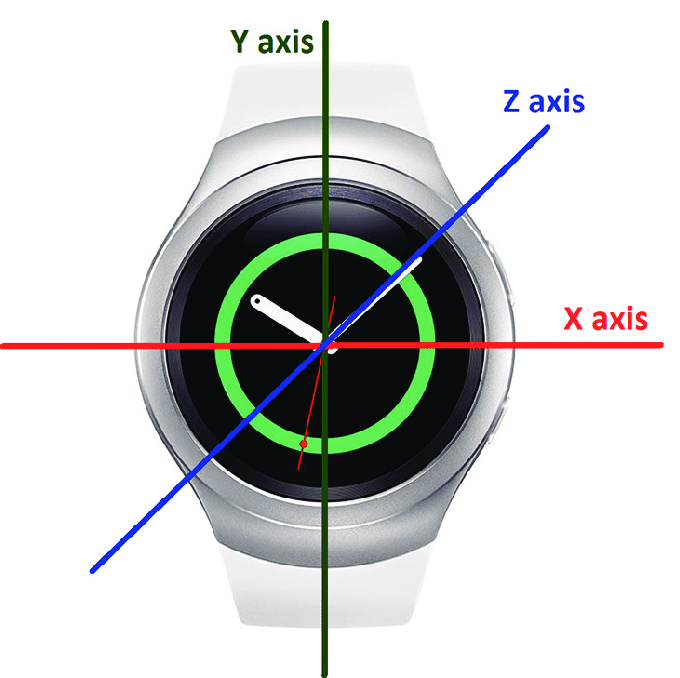
\includegraphics[width=0.5\textwidth]{apparatuur/Smartwatch-accelerometer-axes.png} 
  }
  \ffigbox[\FBwidth]{\caption{Polar M600  \cite{ref24}}\label{fig:polarM600}}{%
    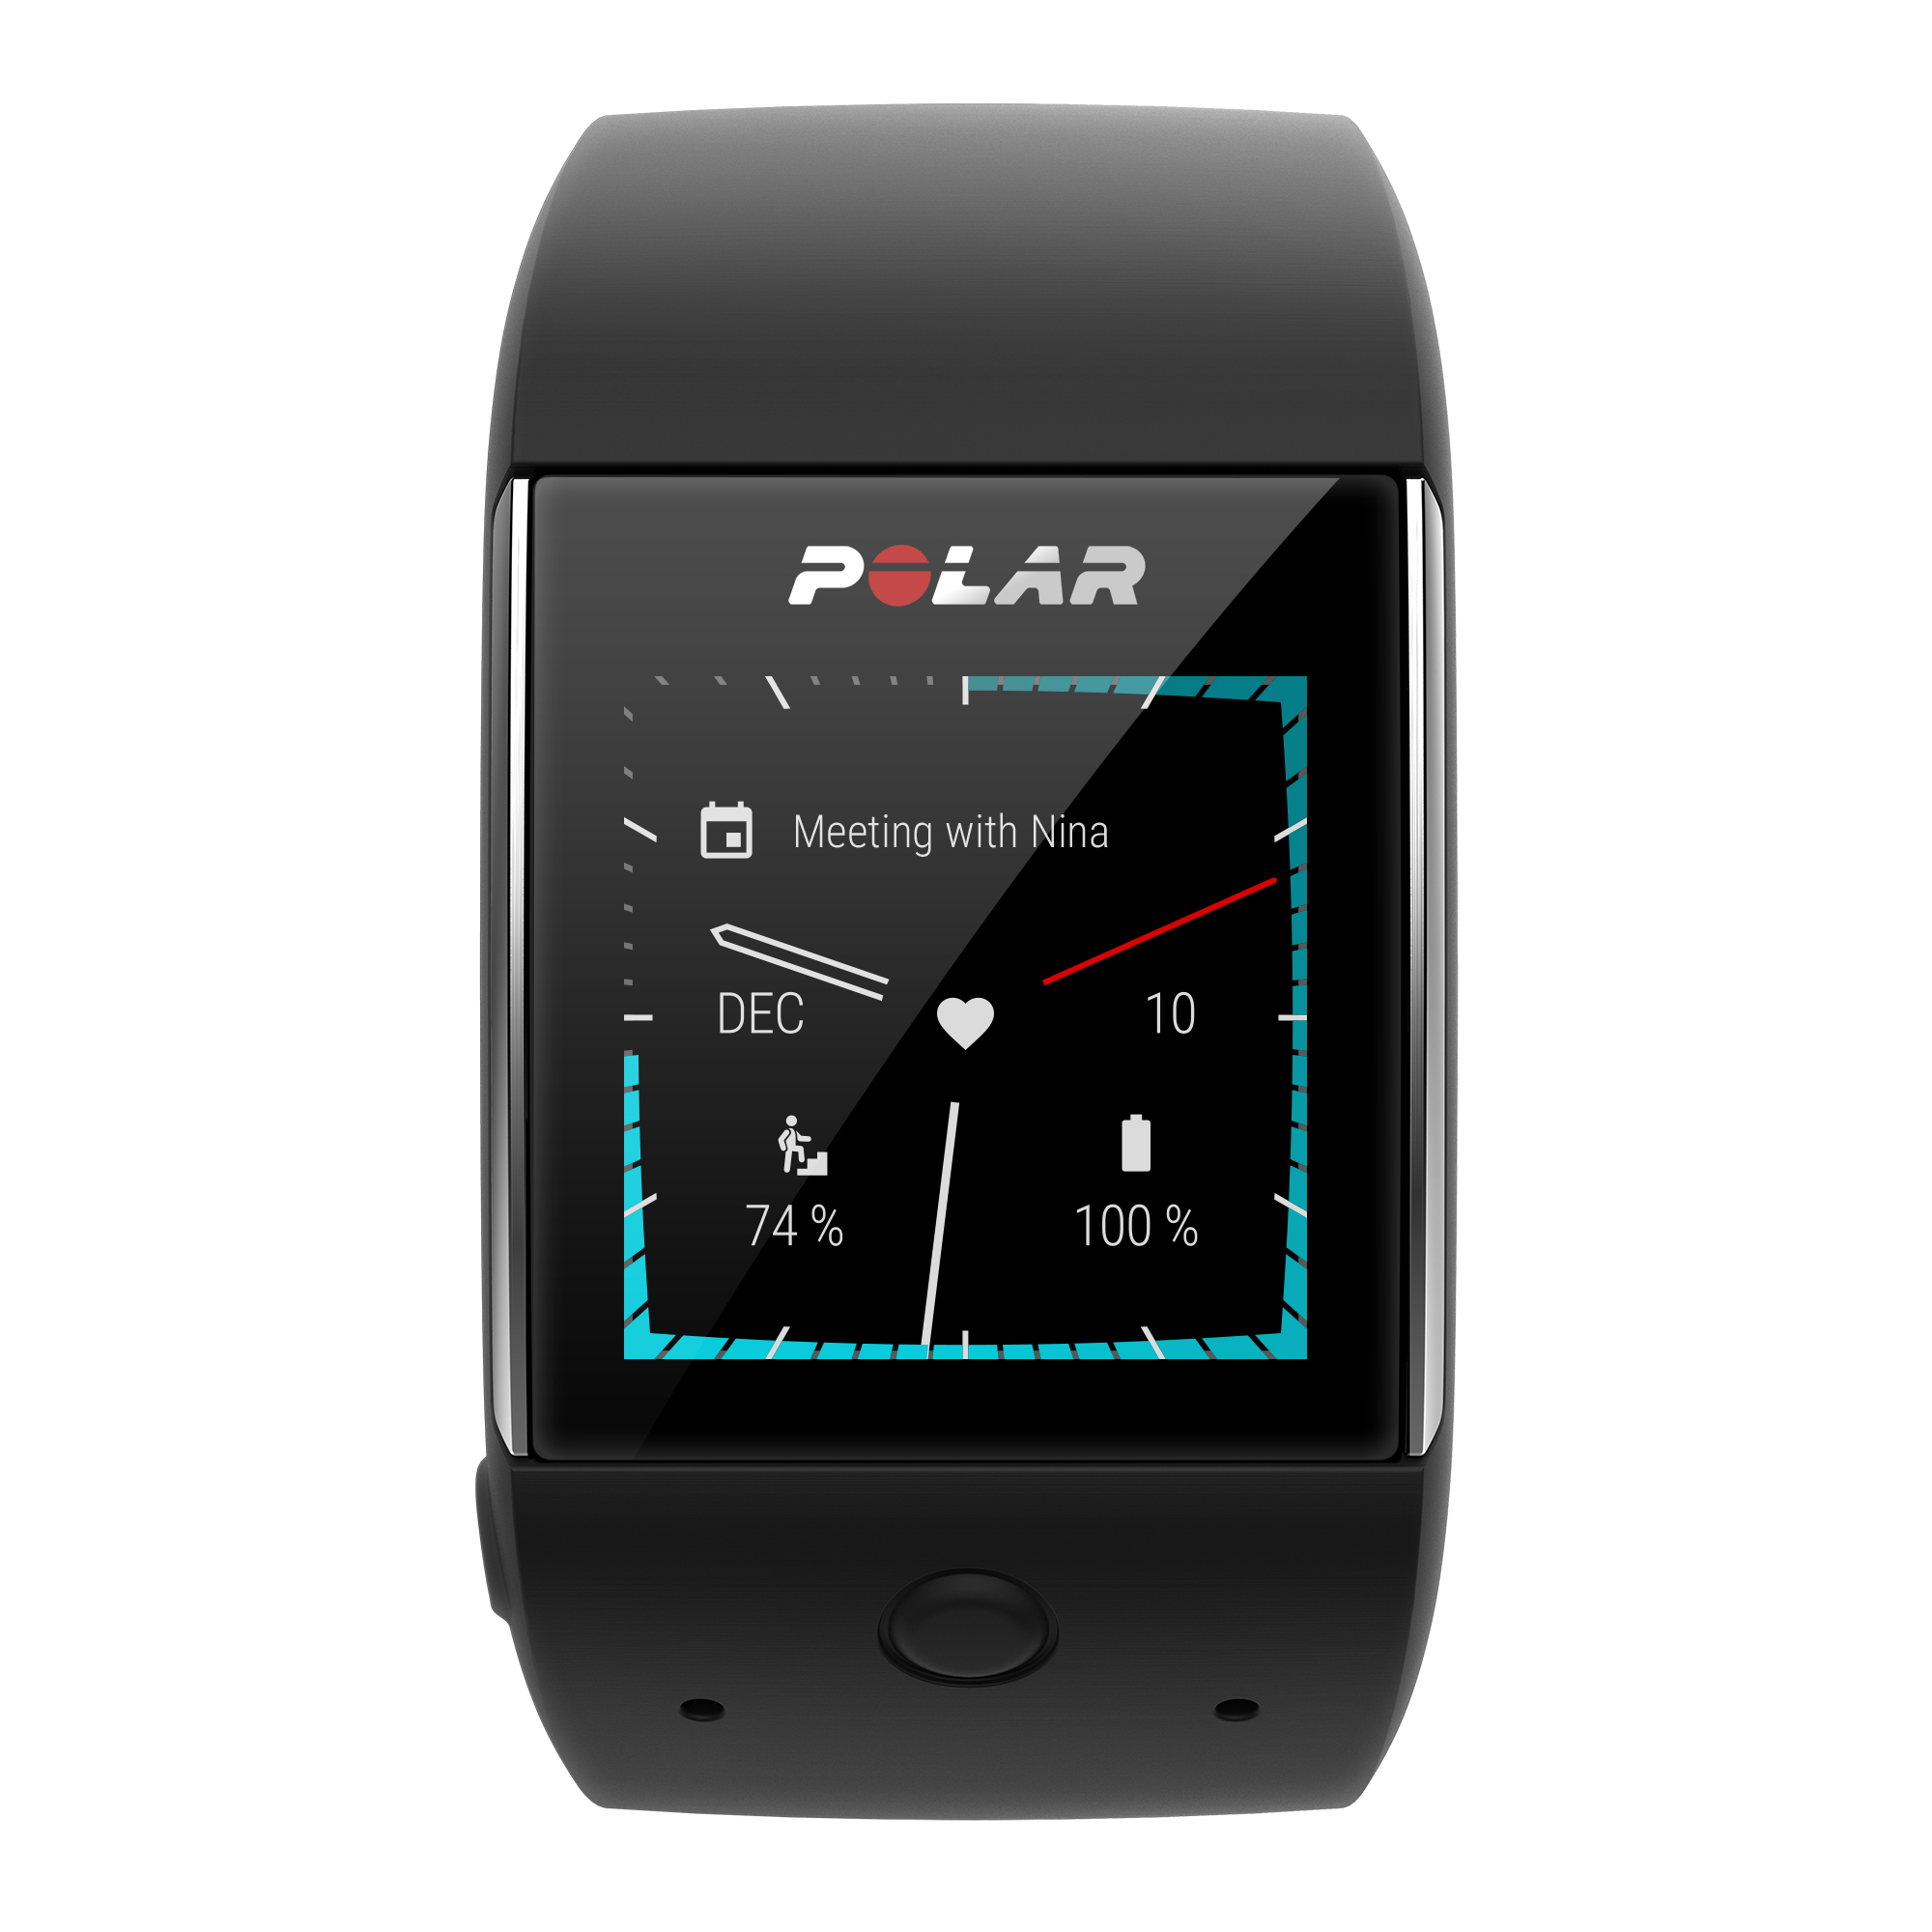
\includegraphics[width=0.5\textwidth]{apparatuur/polarM600.jpg}
  }
\end{floatrow}
\end{figure}

\subsection{Android smartphone}
Tijdens dit onderzoek werd gebruik gemaakt van een Huawei Nova voor het ontwikkelen en testen van de uiteindelijke applicatie alsook tijdens het data verzamelingsproces.  

\section{Sensoren}
Voor het herkennen van beweging is bepaalde data nodig afkomstig van sensoren. Ook is de bepaling van persoonlijke aanbevelingen afhankelijk van hartslagdata eveneens afkomstig van een sensor. Om deze redenen worden de gebruikte sensoren en hun interne werking kort toegelicht.

\subsection{Accelerometer}
Een accelerometer is een sensor gebruikt om versnellingskrachten in kaart te brengen. Deze krachten kunnen zowel statisch, zoals de zwaartekracht, als dynamisch zijn. 
Via kristalstructuren, die gespannen worden onder dwang van versnellingskrachten, wordt een voltage niveau gecreëerd. Via deze waarde is het mogelijk om een oriëntatie en lengte van de corresponderende vector te bepalen \cite{ref54}. Dit proces is te zien op figuur \ref{fig:werkingacc}

In android toestellen wordt typisch met twee verschillende coördinaat systemen gewerkt. Een eerste is een coördinaat stelsel relatief ten opzichte van het toestel. Een tweede vorm is een assenstelsel georiënteerd volgens de aarde.
De android accelerometer sensor gebruikt een 3D assenstelsel georiënteerd volgens de eerste manier, dus ten opzichte van het toestel. In dit soort coördinaten systeem worden de assen niet aangepast bij rotatie van het toestel.
De accelerometer sensor meet de versnelling langs elk van de assen al dan niet samen met de zwaartekracht, afhankelijk van het type sensor. De sensor met type TYPE\_LINEAR\_ACCELERATION houdt geen rekening met de bijdrage van de zwaartekracht. Het type TYPE\_GRAVITY kijkt dan weer enkel naar de zwaartekracht. 
De accelerometer sensor is zeer energiezuinig ten opzichte van andere sensoren wat een groot voordeel is bij langdurig gebruik \cite{ref55}.

\begin{figure}
\centering
\caption{Werking accelerometer \cite{ref56}}\label{fig:werkingacc}
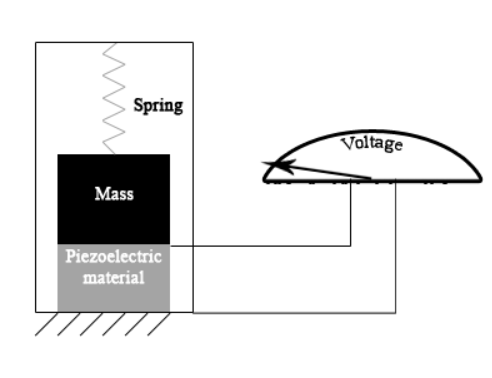
\includegraphics[scale=0.8]{apparatuur/accelerometer_spring.PNG}
\end{figure} 

\subsection{Hartslag sensor}
De Polar M600 utiliseert een optische sensor om hartslag te meten. Hierbij wordt gebruik gemaakt van licht om de bloedcirculatie in beeld te brengen. Een groen licht schijnt op de pols tijdens het meten. Verschillende golflengtes van deze lichtgolf interageren met het bloed. Het uitgezonden licht reflecteert hierop waarna een tweede sensor deze informatie, namelijk het al dan niet reflecteren van de lichtbundel, opvangt \cite{ref57}.

Wanneer bloed circuleert verandert namelijk het volume naarmate meer of minder circulatie aanwezig is. Licht zal minder goed reflecteren indien het bloedvolume hoog is. De tijd tussen lage en hoge gereflecteerde lichtintensiteit wordt gebruikt om de hartslag te berekenen \cite{ref58}. Figuur \ref{fig:hartslagsensor} visualiseert dit proces.

\begin{figure}
\centering
\caption{Werking hartslag sensor \cite{ref59}}\label{fig:hartslagsensor}
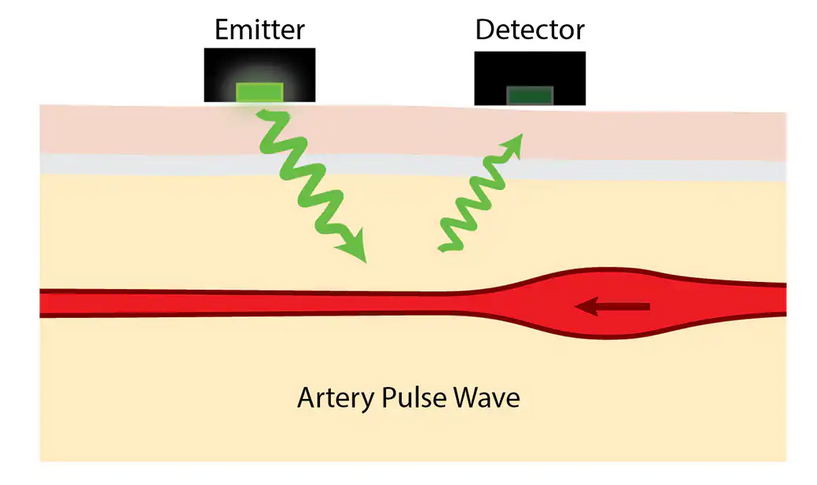
\includegraphics[scale=0.7]{apparatuur/heartrate_emitter.PNG}
\end{figure} 

\section{Software}
Volgende sectie beschrijft de gebruikte \textit{software libraries} en APIs. Hierbij zullen alle technologieën aan bod komen waarmee deze thesis in aanraking gekomen is. Ook zal telkens de reden voor het al dan niet gebruik ervan aangehaald worden.

\subsection{Google fit}
Google fit is een centrale opslagplaats voor fitnessdata waarbij interactie met meerdere applicaties mogelijk is.
De \textit{cloud service} bestaat uit een aantal componenten. Via de Google fit APIs kunnen verschillende high level representaties van elementen bekomen worden. Werken met de Fitstore is hierdoor gemakkelijk. Data Sources zijn één van deze \textit{high level} representaties, deze stellen sensoren voor. Data Types, een andere high level representatie, bevatten info over het soort data (aantal stappen, hartslag...). Data Points is een array van waarden met een bepaald data type, komende vanuit een data source. Datasets zijn datapunten van hetzelfde type van dezelfde source binnen een bepaald tijdsinterval. Sessions, als laatste, stellen een tijdsinterval voor waarin de gebruiker een activiteit beoefent. 
Omdat Google fit omgaat met vertrouwelijke fitness data en deze het toestel verlaat, is toestemming van de gebruiker noodzakelijk \citep{ref10}. \\

\noindent
Er werd gekozen om geen gebruik te maken van Google fit omwille van volgende redenen. Voor de detectie en aanbeveling van activiteiten wordt gebruik gemaakt van een eigen \textit{machine learning model}. Om interactie met Google fit mogelijk te maken zou dus een externe backend server noodzakelijk zijn. 
Ook zal vertrouwelijke fitnessdata het toestel moeten verlaten indien voor Google fit gekozen wordt. 
Google fit is afhankelijk van een werkende internetconnectie om recente data te kunnen weergeven. Een fitness applicatie ontwikkeld om de gebruiker optimaal te stimuleren baat echter voordeel bij een onafhankelijkheid van internet om resultaten in beeld te brengen.

\subsection{Scikit learn}
Scikit learn is een machine learning library voor python. Hierin zijn diverse algoritmes geïmplementeerd voor onder andere classificatie, regressie en unsupervised learning. Ook is het mogelijk om de aangeboden preprocessing functionaliteit te hanteren. Dit bevat onder andere normalisatie implementaties en standaard schalers. Eveneens zijn algoritmes die helpen bij de automatisering van alle stappen in het data analyse proces aanwezig (dimensionality reduction, Feature selection, feature extraction en feature engineering) \cite{ref60}.

\subsection{Google SignIn}
In deze thesis wordt Google SignIn gebruikt als authenticatiemiddel. Via deze weg kan de gebruiker inloggen met zijn/haar Google account. Deze service behoort tot de Google APIs. Er moet hiervoor dus een Google API console project aangemaakt worden. Indien authenticatie met een backend server mogelijk moet zijn, is een OAuth 2.0 client ID vereist. Deze moet meegegeven worden met de Google SignIn opties. 

\subsubsection{OAuth}
OAuth 2.0 is het standaard protocol voor authorizatie van client en server. Dit protocol zorgt voor (gelimiteerde) toegang van \textit{third party} applicaties naar een backend server.
Er zijn vier rollen gedefinieerd in het OAuth protocol. De eerste is \textit{resource owner}, dit is de instantie die de informatie aanvraagt. \textit{Resource server} is de server die uw persoonlijke data beheert. Cliënt is de applicatie die toegang vraagt tot de server. Authorisation server is de server die \textit{access tokens} uitdeelt aan de diverse clients. De rol van resource en \textit{authorisation server} kan door dezelfde machine opgenomen worden. Er wordt gebruik gemaakt van access tokens en \textit{refresh tokens}. Een access token geeft de toegang en moet vertrouwelijk gehouden worden. Refresh tokens worden gebruikt om access token te vernieuwen aangezien deze een beperkte levensduur hebben \cite{ref25}.

\subsection{Wearable Data Layer API}
Met behulp van Wear OS kan een smartwatch direct communiceren met een netwerk zonder gekoppeld te zijn aan een mobiel toestel. Indien er een connectie met een smartphone tot stand gebracht is via bluetooth zal het netwerkverkeer geproxied worden langs deze weg. In het andere geval maakt de smartwatch gebruik van Wi-Fi en cellulaire netwerken.
De Wearable Data Layer API biedt een afzonderlijk communicatie kanaal tussen applicaties aan. 
De API bevat een aantal data objecten die communicatie mogelijk maken. Een Data Item slaat info op en zorgt voor automatische syncing tussen gsm en smartwatch. Een Asset zorgt voor verzending van binaire \textit{blobs} van data. Een MessageClient verzendt berichten, de twee apparaten moeten hiervoor geconnecteerd zijn. Een ChannelClient wordt gebruikt voor verzending van grotere bestanden \cite{ref26}.
Deze thesis maakt enkel gebruik van de messageClient. De informatie die zal verzonden worden via deze weg is namelijk niet van die omvang dat een channelClient noodzakelijk is. Ook is gebruik maken van Data Items niet optimaal. Deze objecten zijn namelijk bedoeld om grotere meer persistente info op te slaan, wat hier niet het geval is. Assets zijn eveneens minder geschikt aangezien ze vooral worden gebruikt om afbeeldingen over te dragen.

\subsection{Firebase}
Firebase is een NoSQL document georiënteerde databank, data wordt opgeslagen in documenten die samen zitten in collecties. De databank is bijgevolg schemaloos. De collecties en documenten worden impliciet gecreëerd \cite{ref61}.
Gebruik van Firebase als opslagplaats voor sensor data is zeer duur. Firebase is namelijk betalend indien een bepaalde dagelijkse limiet overschreden wordt. Voor de opslag van sessie berekeningen is dit eveneens niet zeer geschikt om dezelfde reden als Google fit. Er is namelijk een internetconnectie noodzakelijk om weergave van recente berekeningen mogelijk te maken.

\subsection{Pandas framework}
Pandas is een data analyse library voor python. Het maakt gebruik van \textit{dataframe} objecten voor data manipulatie. Deze datastructuur maakt het mogelijk om de data voor te stellen in rijen van observaties en kolommen van variabelen \cite{ref27}.

\subsection{Tensorflow}
Tensorflow is een end-to-end platform voor het bouwen en \textit{deployen} van Machine Learning modellen. Dit framework maakt het mogelijk om neurale netwerken te ontwikkelen met vele lagen. Voor het bouwen en trainen van deep learning modellen maakt Tensorflow gebruik van Keras \cite{ref62}.

\subsubsection{Tensorflow Lite}

Tensorflow Lite is een manier om machine learning modellen te deployen op mobiele toestellen. Via de Tensorflow lite converter wordt een model geschreven in python geconverteerd naar het LITE formaat. Wanneer dit lite model gedeployed is, kunnen voorspellingen gemaakt worden aan de hand van een interpreter. De voorspelde data moet van dezelfde vorm zijn als waarop het model getraind heeft. Deze info kan verkregen worden via de inputtensor. Er mogen slechts een selectief aantal primitieve types gebruikt worden als input. Sensor data heeft echter telkens een float type wat ondersteund wordt. 
Als output wordt een array van probabiliteiten teruggegeven waarin de indices overeenkomen met de labelindices van het model \cite{ref63}.

\subsection{Workmanager} \label{subsection:workmanager}
Workmanager wordt gebruikt om in de achtergrond taken uit te voeren die niet op één specifiek moment moeten gebeuren. Met andere woorden ze zijn uitstelbaar. Dit is nodig om ervoor te zorgen dat de taken op een zo efficiënt mogelijke manier kunnen uitgevoerd worden. Er kan bijvoorbeeld gewacht worden tot het mobiele toestellen oplaadt of totdat de accu boven een zekere waarde stijgt. Een eerste manier om zogenoemde \textit{workrequests} te definiëren is met een OneTimeWorkRequest. Dit soort \textit{request} zorgt ervoor dat de taak, na een optionele vertraging, zo snel mogelijk en zo efficiënt mogelijk uitgevoerd wordt. Een andere manier, optimaal voor taken die telkens opnieuw moeten gerealiseerd worden, is via een PeriodicWorkRequest. Hiermee wordt een interval gespecificeerd waarin de taak kan uitgevoerd worden. Indien een kleiner tijdsinterval gewenst is, kan gebruik gemaakt worden van een \textit{flexinterval}. Dit zorgt ervoor dat de taak niet op eender welk moment binnen het globale interval mag uitgevoerd worden, maar enkel binnen het flexinterval. Via een instantie van het WorkManager object kunnen de verschillende requests gequeued worden (zie figuur \ref{fig:periodicwork}). Het is eveneens mogelijk om een bepaalde unieke job te behouden of om deze telkens te vervangen door een nieuw exemplaar. Dit om te voorkomen dat verschillende instanties van eenzelfde taak aanwezig zijn \cite{ref64}.

Toegepast op deze thesis kan Workmanager zeker zijn nut bewijzen. De berekening van nieuwe aanbevelingen gebaseerd op additionele fitnessdata zal namelijk periodiek gebeuren. Een andere optie was om telkens de aanbevelingspagina gerefreshed wordt, alle berekeningen van nul te herbeginnen. Dit zou een bottleneck kunnen vormen voor het systeem, vandaar de keuze voor Workmanager.

\begin{figure}
\centering
\caption{PeriodicWorkRequest \cite{ref65}}\label{fig:periodicwork}
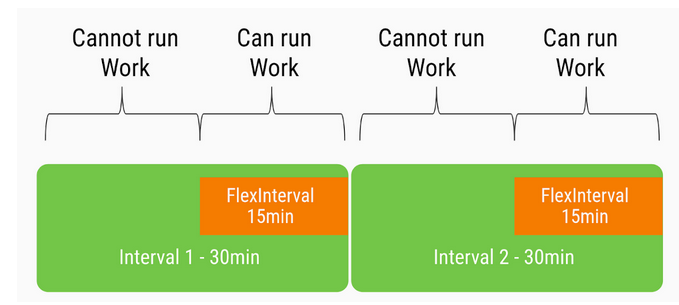
\includegraphics[scale=0.6]{apparatuur/periodicWorkRequest.PNG}
\end{figure} 

\subsection{Room}

De Room Persistence Library maakt onderliggend gebruikt van SQLite, maar biedt nog een extra abstractie laag voor gebruiksgemak. SQLite is een zeer kleine, \textit{lightweight database} waardoor het zicht zeer goed leent tot gebruik in mobiele toestellen. SQLite vereist ook geen speciale database server, het maakt gebruik van een filesysteem in SQL syntax \cite{ref66} \cite{ref67}.
Er werd gekozen voor een volledige lokale implementatie. Hierbij staat Room als opslagplaats centraal. De database wordt gebruikt om allerhande fitnessdata in te bewaren. Er zal rekening gehouden worden met de maximale capaciteit door tijdig historische data ouder dan tien weken te verwijderen. Dit heeft geen negatieve invloed op de werking van de applicatie aangezien deze ontworpen is voor een tien weken durende training.


\graphicspath{ {./rope_skipping/} }

\chapter{Rope skipping} \label{chapter:3}
In deze studie wordt gefocust op rope skippen als middel om beweging toegankelijk te maken. Rope skipping is een ideale sport om de conditie te trainen.
Aan de hand van de herkenning en classificatie van rope skipping bewegingen, met gelijktijdige monitoring van hartslag data, kan een schatting gemaakt worden van het inspanningsniveau. Gebruikers krijgen persoonlijke aanbevelingen te zien om een optimale conditietraining te verzekeren. Minder frequente en/of minder lange trainingsessies zullen aangeboden worden bij onervaren rope skippers. Gebruikers worden eveneens aangemoedigd om bewegingen waarin fouten gemaakt werden meer in te oefenen.
In wat volgt wordt beschreven hoe bovenstaande technieken verwezenlijkt worden. Machine learning ligt hierbij aan de basis. Verschillende machine learning algoritmen komen dan ook uitvoerig aan bod alsook voorafgaande preprocessing van de data. Om nuttige statistieken te kunnen tonen, is data manipulatie van onbewerkte accelerometer data essentieel.
Het onderzoek naar de classificatie van rope skipping bewegingen bestaat uit het analyseren van de diverse bewegingen en in hoeverre deze van elkaar te onderscheiden zijn. Verschillende machine learning algoritmes worden getest om zo het meest optimale algoritme voor deze casus te bekomen. Hierbij wordt gefocust op accelerometer data. 
 
\section{Bewegingen}
Dit onderdeel heeft als doel de onderzochte bewegingen toe te lichten. De bewegingen op zich worden uitgelegd aan de hand van afbeeldingen. Om een zo correct mogelijk beeld te verkrijgen van deze bewegingen, wordt gewerkt met data afkomstig van verschillende proefpersonen met verschillend vaardigheidsniveau en van diverse leeftijden (21 - 73 jaar). De gelijkenissen en verschillen tussen bewegingen worden aangekaart. Er wordt telkens gebruik gemaakt van een tien seconden interval tijdens de analyse.
Aangezien bij een draaiende beweging de versnelling wordt veroorzaakt door de centripetale kracht en deze loodrecht op de snelheidsvector staat, is het intuïtief niet zo eenvoudig om dit te analyseren. Niettegenstaande wordt een poging ondernomen.

\subsection{Springen met tussensprong (jump slow)} \label{jumpslow}

\begin{figure}[!htpd]
\centering
\caption{Proefpersoon 1: springen met tussensprong}\label{fig:jump_slow1}
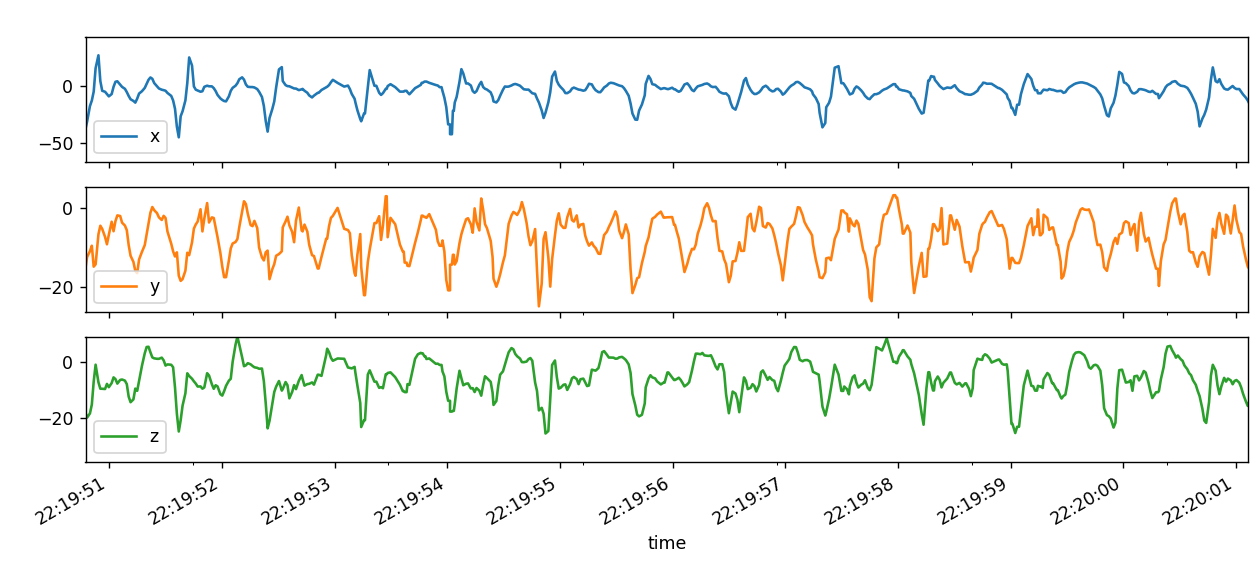
\includegraphics[width=.9\textwidth]{rope_skipping/jump_slow_proefpersoon1.PNG}
\end{figure}

\begin{figure}[!htpd]
\centering
\caption{Proefpersoon 2: springen met tussensprong}\label{fig:jump_slow2}
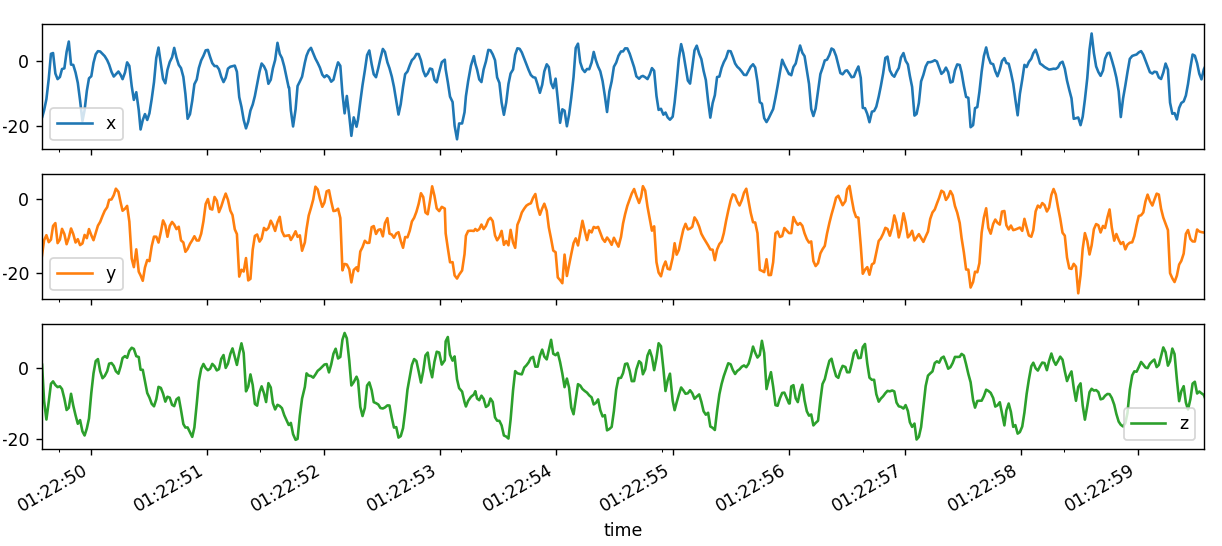
\includegraphics[width=.9\textwidth]{rope_skipping/jump_slow (10 sec).PNG}
\end{figure}

Bij springen met tussensprong zal er met iedere draaiing van het touw twee keer gesprongen worden.
In bovenstaande Figuren is het verloop te zien van de verschillende accelerometer assen tijdens het springen. Er is een duidelijk periodiek verloop merkbaar. Één periode staat gelijk aan één enkele draaiing. 
Door de tussensprong is de periode op alle drie de grafieken schijnbaar opgedeeld in twee stukken. Een tussensprong veroorzaakt namelijk een extra beweging langs alle drie de assen. 
Ook is de versnelling grotendeels negatief wat aangeeft dat er een grotere snelheidsverandering is bij beweging in de richting van de negatieve assen.

\subsubsection{Vergelijking proefpersonen}
Op Figuur \ref{fig:jump_slow1} en \ref{fig:jump_slow2} zijn signalen te zien van twee verschillende proefpersonen die dezelfde sprong uitvoeren. Alhoewel globaal een overeenkomstige vorm terugkeert, zijn er toch duidelijke verschillen merkbaar en dit vooral op de x en z as. Op de z as is te zien dat proefpersoon 1 in de eerste helft van een draaiing een grote versnelling heeft. Bij proefpersoon 2 is dit juist omgekeerd. Op de x as is te zien dat proefpersoon 1 een nagenoeg constante snelheid aanhoudt tijdens een periode. Proefpersoon 2 veroorzaakt op een gegeven moment tijdens een draaiing een kortstondige versnellingspiek. Dit kan te wijten zijn aan het al dan niet uitgesproken zijn van de tussensprong.

\subsection{Springen zonder tussenprong (jump fast)}

\begin{figure}[!htpd]
\centering
\caption{Proefpersoon 1: springen zonder tussensprong}\label{fig:jump_fast1}
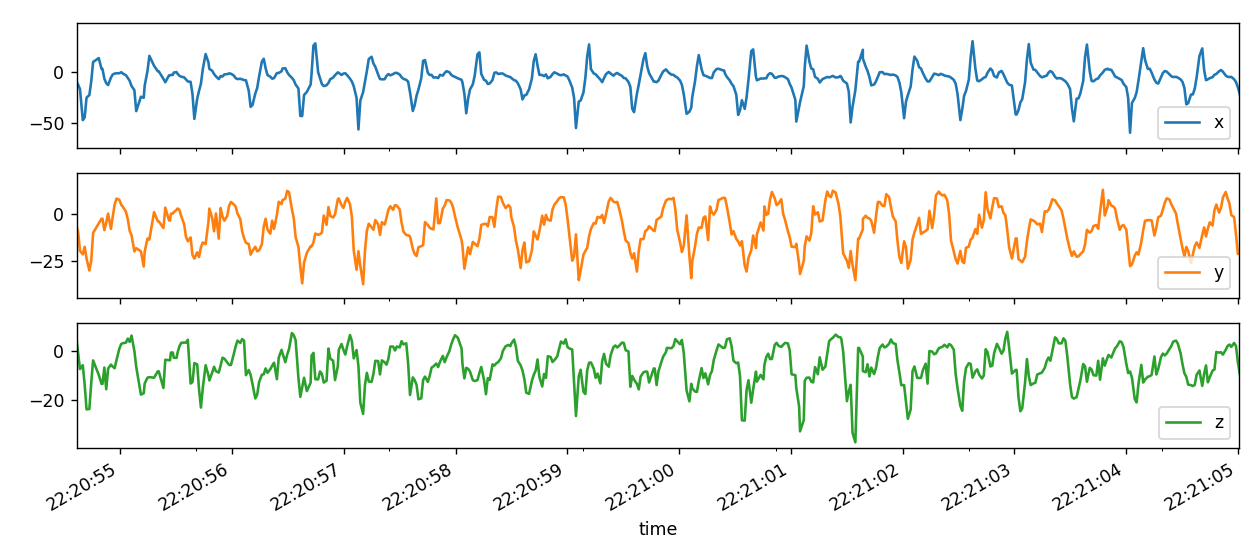
\includegraphics[width=.9\textwidth]{rope_skipping/jump_fast(proefpersoon1).PNG}
\end{figure}

\begin{figure}[!htpd]
\centering
\caption{Proefpersoon 2: springen zonder tussensprong }\label{fig:jump_fast2}
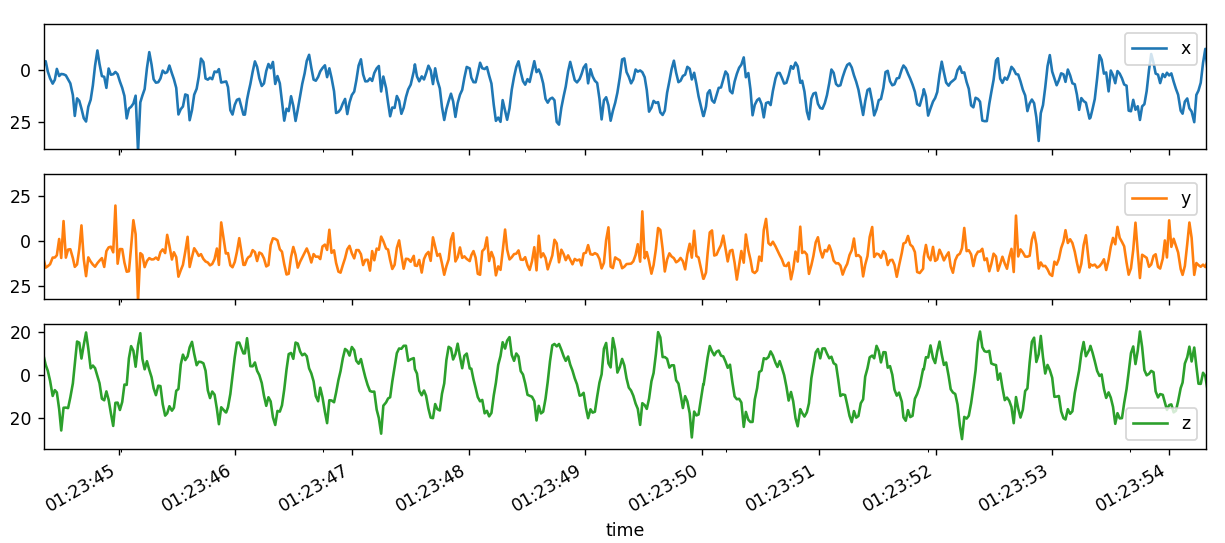
\includegraphics[width=.9\textwidth]{rope_skipping/jum_fast (10 sec).PNG}
\end{figure}

Bij deze beweging vindt er tijdens elke draaiing van het touw één sprong plaats in plaats van twee. Dit resulteert in een kleinere periode en grotere frequentie. 
Het signaal op de x-as is ook weer voor het grootste deel negatief. Dit is niet het geval voor de andere assen.

\subsubsection{Vergelijking proefpersonen}
Figuren \ref{fig:jump_fast1} en \ref{fig:jump_fast2} tonen de accelerometer signalen.
De y-as is een goede indicator voor de grootte van de polsbeweging tijdens een sprong aangezien er minder versnelling zal zijn langs die as bij kleinere draaiingen. Deze as staat namelijk voor het grootste deel van één periode naar boven gericht (zie subsectie \ref{polar}). Proefpersoon 2 maakt bijgevolg kleinere draaiingen in vergelijking met proefpersoon 1.

\subsection{Jump run}

\begin{figure}[!htpd]
\centering
\caption{Proefpersoon 1: jump run}\label{fig:jump_run1}
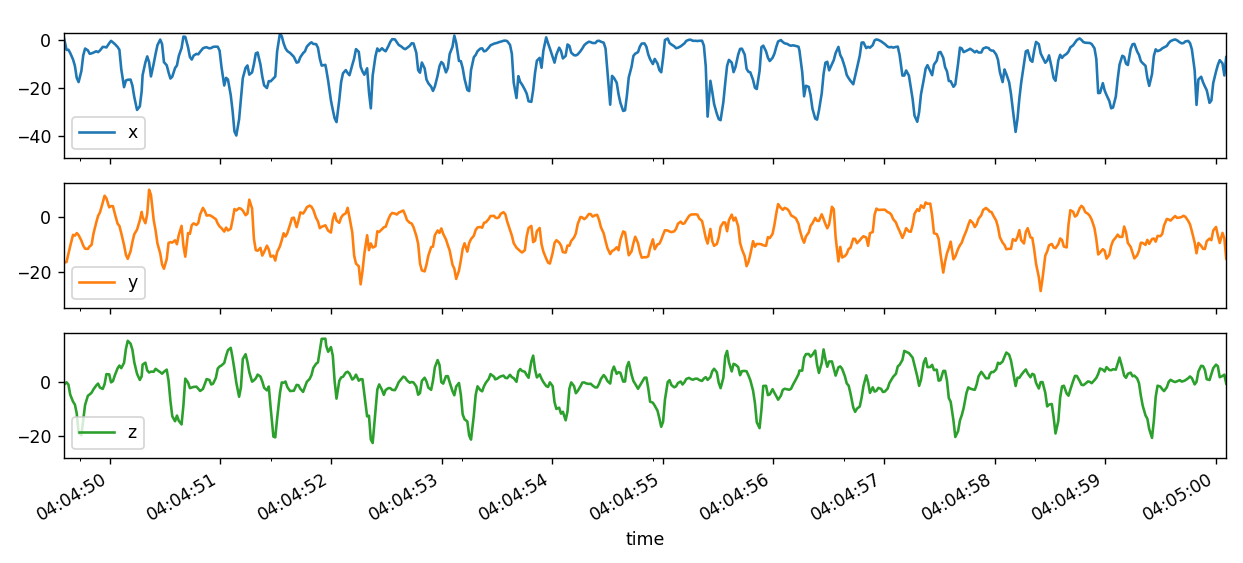
\includegraphics[width=.9\textwidth]{rope_skipping/jump_run_proefpersoon1.PNG}
\end{figure}

\begin{figure}[!htpd]
\centering
\caption{Proefpersoon 2: jump run}\label{fig:jump_run2}
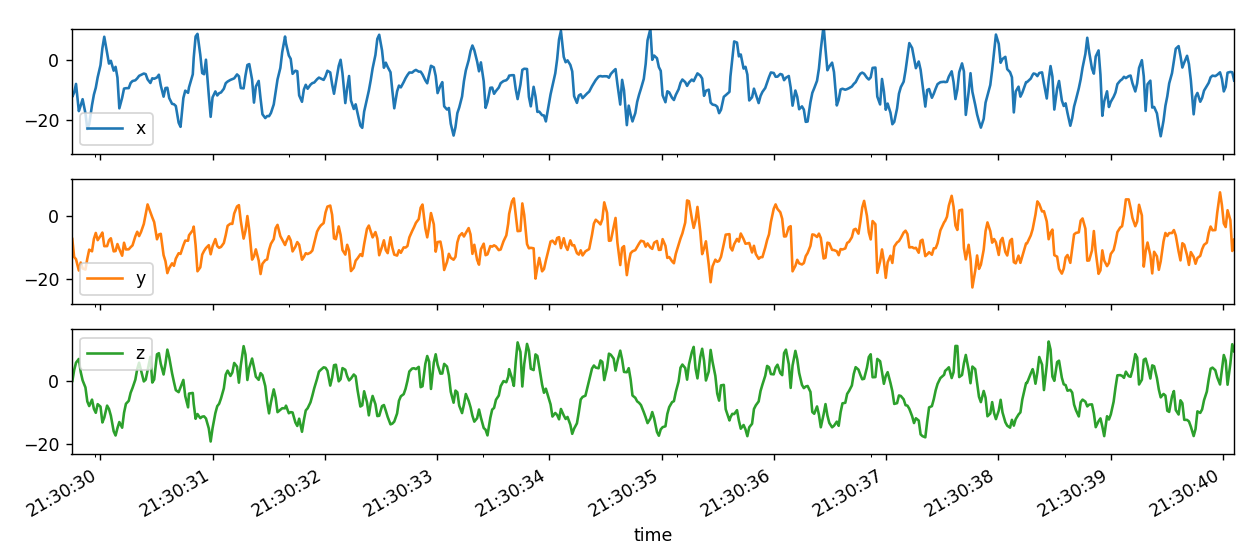
\includegraphics[width=.9\textwidth]{rope_skipping/jump_run_proefpersoon2.PNG}
\end{figure}

Deze beweging is een combinatie van lopen en springen met tussensprong. Er wordt met andere woorden al springend gelopen. Indien deze signalen vergeleken worden met de beweging: springen met tussensprong, dan kan opgemerkt worden dat deze toch wel enige gelijkenissen vertonen. Dit is zeker logisch aangezien een jump run eigenlijk bestaat uit springen met tussensprong aangevuld met verplaatsing. Toch is er een onderscheid en dit is vooral merkbaar op de x-as.

\subsubsection{Vergelijken proefpersonen}
De onderlinge verschillen, te zien op Figuren \ref{fig:jump_run1} en \ref{fig:jump_run2}, zijn gelijkaardig aan deze aangekaart in subsectie \ref{jumpslow}. Aangezien de x-as de meeste verschillen toont, zal deze besproken worden. Proefpersoon 2 vertoont hierbij een grilliger verloop wat aangeeft dat de mate van versnelling vaak verandert langs deze as. 

\subsection{Cross over}

Cross over is een beweging waarbij gesprongen wordt met de armen gekruist. Een illustratie hiervan is te zien op Figuur \ref{fig:crossover}. Tijdens dit onderzoek werd ervoor gekozen om te focussen op cross over met tussensprong. Dit door het tekort aan proefpersonen die in staat zijn de snellere en intensievere versie hiervan uit te voeren.
Op Figuur \ref{fig:cross_over1} is duidelijk te zien dat de amplitude langs de x-as veel kleiner is. De x-as loopt namelijk evenwijdig met de arm en aangezien de armen in een nogal geklemde positie zitten is beweging langs deze as moeilijker (zie subsectie \ref{polar}). Verder is er ook weer een periodiek verloop merkbaar, al is dit wat minder uitgesproken.
X- en y-as ondergaan vooral een versnelling in negatieve richting. De z-as daarentegen ondergaat doorgaans een positieve versnelling.
Aangezien er een tekort aan proefpersonen is die bekwaam zijn om deze beweging uit te voeren, is het niet mogelijk om een onderlinge vergelijking te maken.

\begin{figure}[!htpd]
\centering
\caption{Proefpersoon 1: cross over}\label{fig:cross_over1}
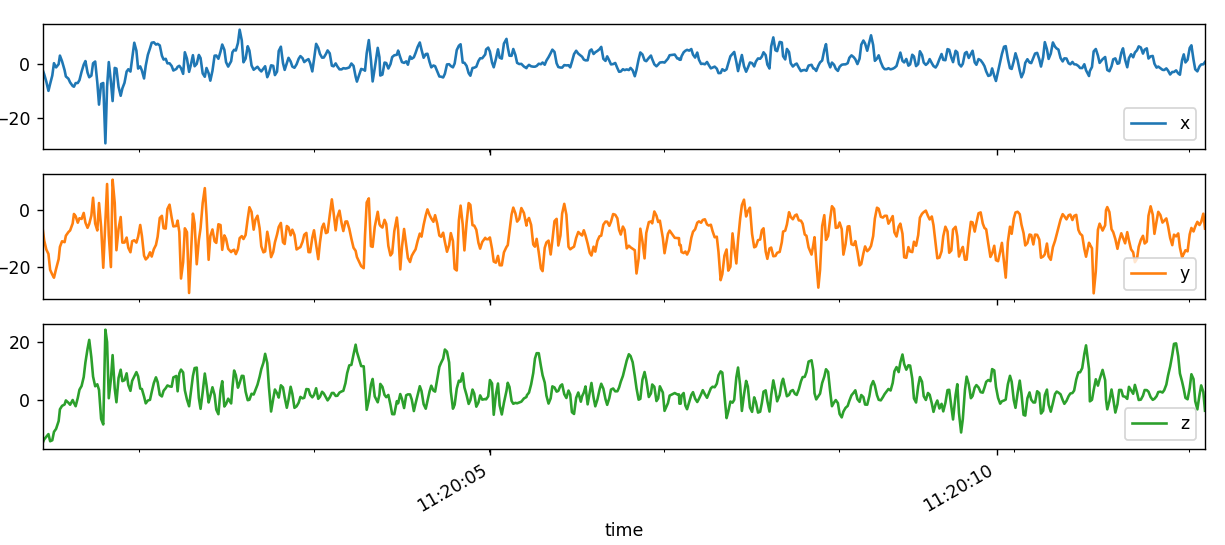
\includegraphics[width=.9\textwidth]{rope_skipping/crossover (10 sec).PNG}
\end{figure}

\subsection{Side swing} \label{subsection:sideswing}

Side swing (zie Figuur \ref{fig:sideswing}) is een beweging waarbij de uitvoerder het touw één maal rechts van hem/haar ronddraait en meteen hierna één maal links. Er kan ook voor gekozen worden om links te beginnen en rechts te eindigen.
Ook in dit signaal is een periodiek verloop merkbaar (zie Figuren \ref{fig:side_swing1} en \ref{fig:side_swing2}). De verandering in snelheid langs de verschillende assen verloopt echter trager. De armen en polsen zijn tijdens deze beweging namelijk compleet vrij zodat op elke as duidelijke veranderingen in richting zichtbaar zijn.
Aan de waarden is te zien dat deze kleiner zijn. Dit komt omdat side swing een rustige beweging is met minder bruuske snelheidsveranderingen. Ook dit verloop is in twee stukken verdeeld op x- en y-as doordat dezelfde beweging langs beide kanten van het lichaam moet uitgevoerd worden. De z-as daarentegen vertoont een ander soort patroon. 

\subsubsection{Vergelijken proefpersonen}
Het verloop van de y- en z-as is zeer gelijkaardig. De x-as daarentegen vertoont enkele verschillen. Proefpersoon 1 toont een duidelijker patroon in vergelijking met proefpersoon 2. Dit tweede signaal bevat namelijk enkele pieken.

\begin{figure}[!htpd]
\centering
\caption{Proefpersoon 1: side swing}\label{fig:side_swing1}
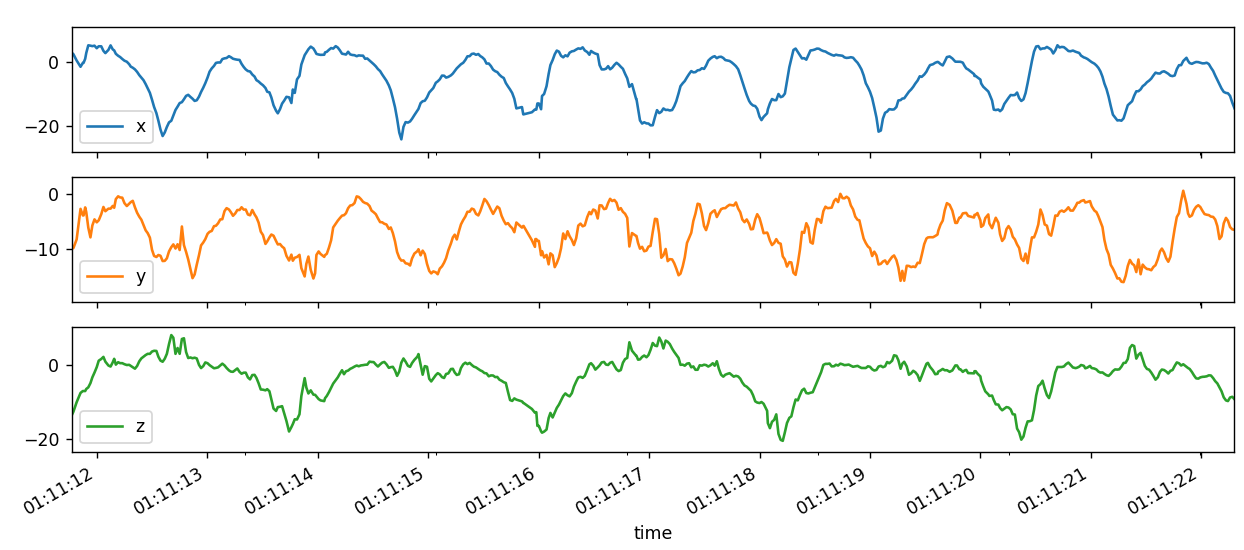
\includegraphics[width=.9\textwidth]{rope_skipping/side_swing_proefpersoon1.PNG}
\end{figure}

\begin{figure}[!htpd]
\centering
\caption{Proefpersoon 2: side swing}\label{fig:side_swing2}
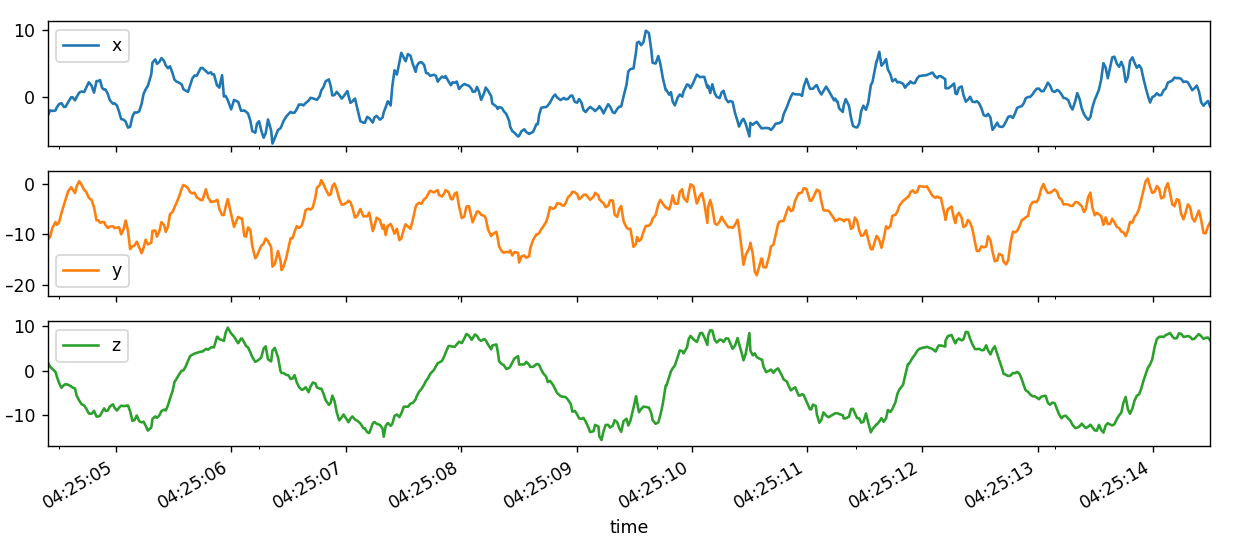
\includegraphics[width=.9\textwidth]{rope_skipping/side-swing (10 sec).PNG}
\end{figure}

\subsection{Forward 180}
Deze beweging zorgt ervoor, zoals de naam zegt, dat de uitvoerder zichzelf 180 graden draait tijdens het springen (zie Figuur \ref{fig:forward180}). Dit wordt verwezenlijkt door met behulp van een side swing tijdens het draaien het touw op de juiste plaats te krijgen. Wanneer men gedraaid is kan achterwaarts verder gesprongen worden.
Het meten van deze beweging was iets moeilijker aangezien dit niet constant achter elkaar kan uitgevoerd worden. Een oplossing bestond erin om na iedere achterwaartse sprong, het touw van richting te veranderen. 
Het periodiek verloop is terug zichtbaar doordat dezelfde beweging telkens opnieuw werd uitgevoerd (zie Figuren \ref{fig:forward_1801} en \ref{fig:forward_1802}).
De ruis die te zien is tussen twee perioden door (vooral langs de y-as) heeft te maken met het feit dat na één beweging, zoals vermeld, van richting moet veranderd worden. De handen moeten bijgevolg terug in positie gebracht worden.
Ook hier is de grafiek weer in twee delen verdeeld. Er zijn tijdens deze beweging eveneens twee sprongen nodig met daartussen een side swing als overgangsbeweging.
De richting van de versnellingsvector is hoofdzakelijk negatief langs de x- en y-as. 

\subsubsection{Vergelijken proefpersonen}
Zoals vermeld bestaat deze beweging uit twee sprongen en een halve side swing. De y-as vertoont een grote gelijkenissen tussen de twee signalen. De x- en z-as vertonen bij proefpersoon 1 een eerder statisch verloop met enkele pieken in tegenstelling tot proefpersoon 2. 

\begin{figure}[!htpd]
\centering
\caption{Proefpersoon 1: forward 180}\label{fig:forward_1801}
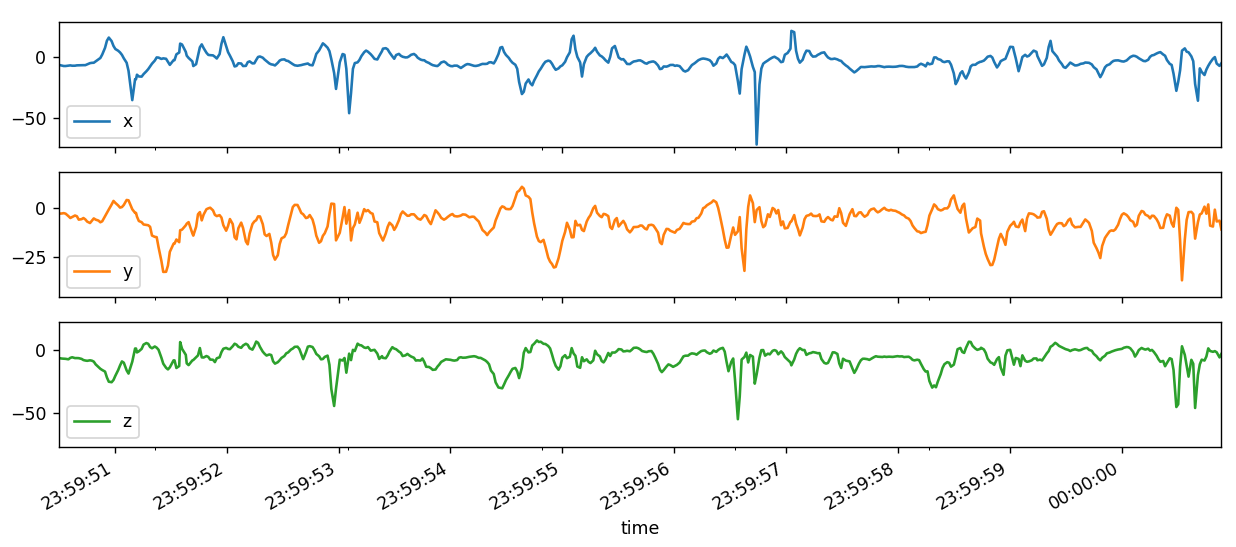
\includegraphics[width=.9\textwidth]{rope_skipping/forward_180_proefpersoon1.PNG}
\end{figure}

\begin{figure}[!htpd]
\centering
\caption{Proefpersoon 2: forward 180}\label{fig:forward_1802}
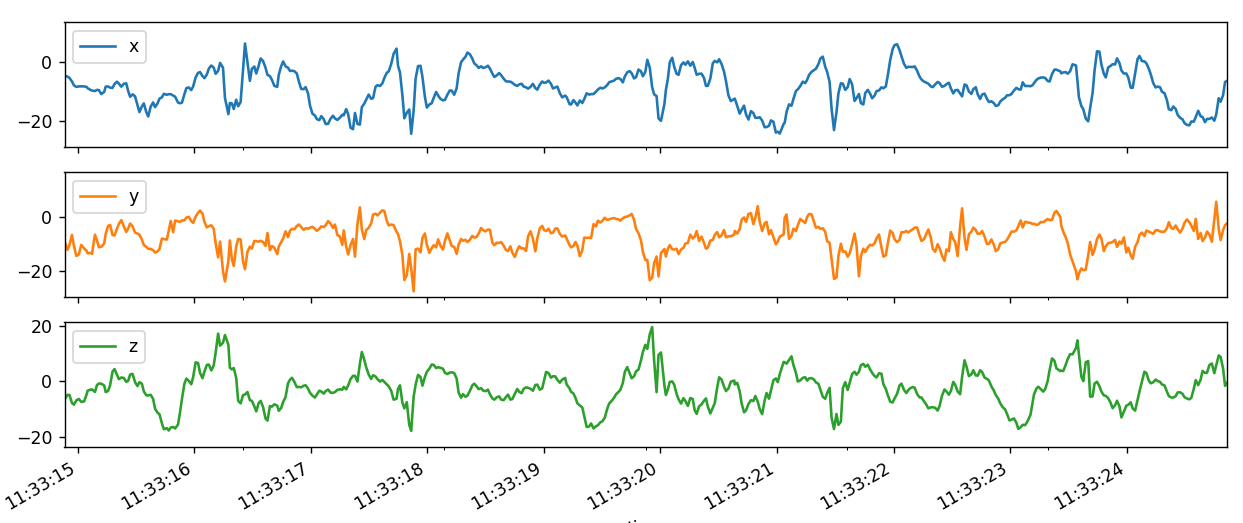
\includegraphics[width=.9\textwidth]{rope_skipping/forward-180 (10 sec).PNG}
\end{figure}

\subsection{Backward 180}
De backward 180 is gelijkaardig aan de forward 180 in zijn uitvoering met als verschil de start-draaiing. Er wordt namelijk gestart vanuit achterwaarts springen. Wanneer het touw zich voor de springer bevindt, draait deze zich 180 graden. Er wordt vervolgens verder voorwaarts gesprongen. Deze beweging bestaat eveneens uit twee sprongen, zonder de aanwezigheid van een halve side swing. Op alle drie de assen is vooral een negatieve versnelling merkbaar. 

\subsubsection{Vergelijken proefpersonen}
Figuren \ref{fig:backward_1801} en \ref{fig:backward_1802} tonen het accelerometer signaal.
De twee signalen lijken in dit geval zeer sterk op elkaar. Enkel komt de iets statischere gedaante van proefpersoon 1 hier weer terug.

\begin{figure}[!htpd]
\centering
\caption{Proefpersoon 1: backward 180}\label{fig:backward_1801}
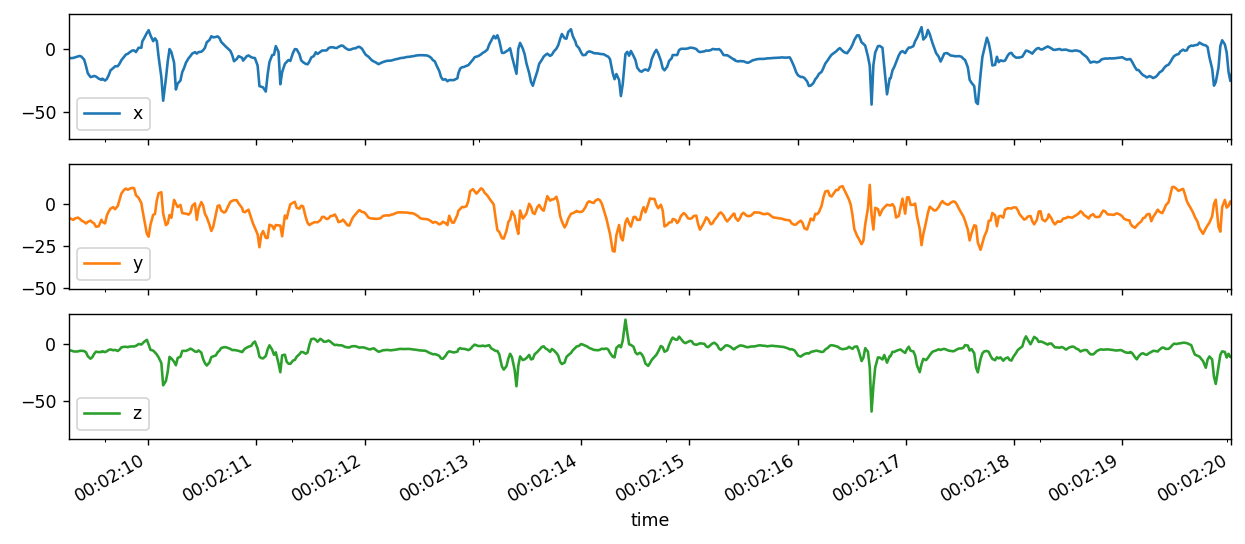
\includegraphics[width=.9\textwidth]{rope_skipping/backward180_proefpersoon1.PNG}
\end{figure}

\begin{figure}[!htpd]
\centering
\caption{Proefpersoon 2: backward 180}\label{fig:backward_1802}
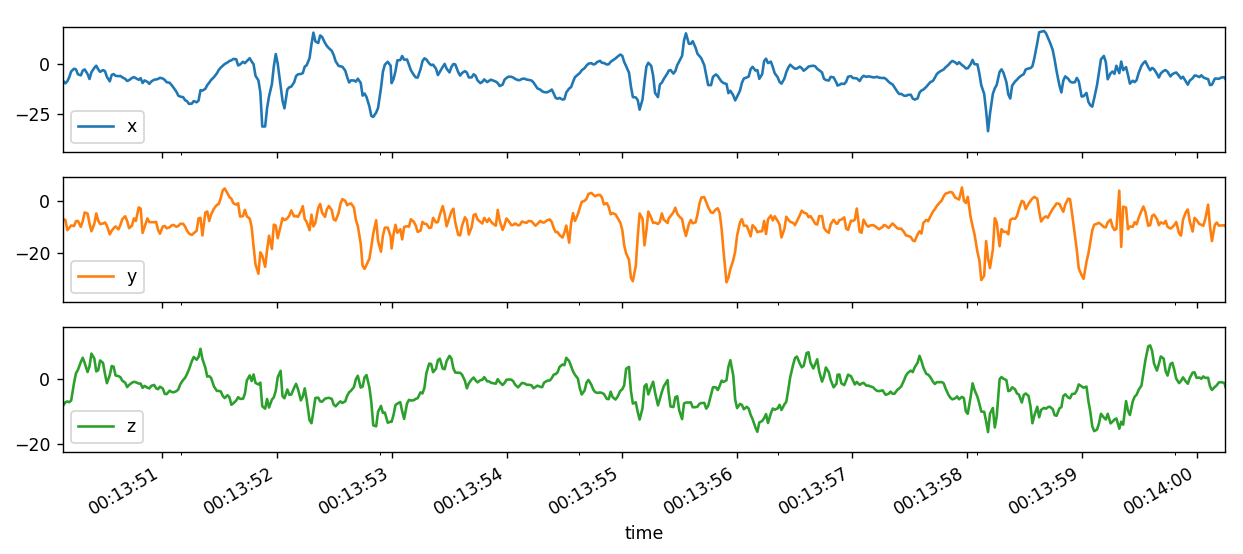
\includegraphics[width=.9\textwidth]{rope_skipping/backward180_proefpersoon2.PNG}
\end{figure}

\begin{figure}[!htpd]
\centering
\begin{floatrow}
  \ffigbox[\FBwidth]{\caption{Cross over \cite{ref82}}\label{fig:crossover}}{%
    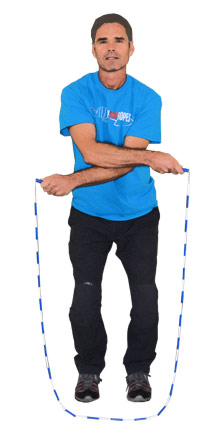
\includegraphics[scale=0.25]{rope_skipping/crossover.jpg} 
  }
  \ffigbox[\FBwidth]{\caption{Side swing \cite{ref82}}\label{fig:sideswing}}{%
    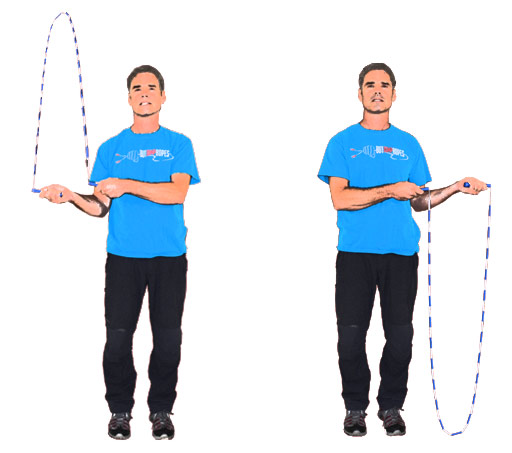
\includegraphics[scale=0.25]{rope_skipping/side-swing.jpg}
  }
  \ffigbox[\FBwidth]{\caption{Forward 180 \cite{ref82}}\label{fig:forward180}}{%
     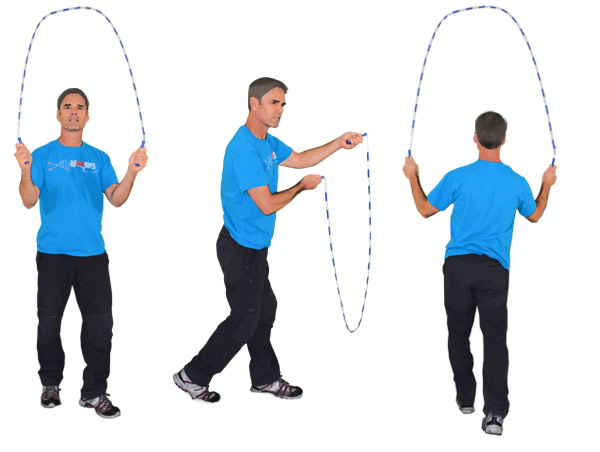
\includegraphics[scale=0.25]{rope_skipping/forward-180.jpg}
  }
\end{floatrow}
\end{figure}

\section{Data collectie} \label{sectie:datacollectie}
Het Polar flow platform laat niet toe om voor een sessie de onbewerkte data te downloaden \cite{ref28}. Hierdoor werd een eigen applicatie ontwikkeld op de smartwatch en smartphone. De smartwatch applicatie zal via sensoren de datapunten opvangen met een sampling frequentie van ongeveer 52 Hz. 

Dit is echter zeer systeem en tijd afhankelijk. Het android systeem en/of andere applicaties kunnen de frequentie ten alle tijde aanpassen. De sampling frequentie kan, afhankelijk van de \textit{lifecycle} waarin de applicatie zit, zelfs verlaagd worden tot 18 Hz \cite{ref68}. Het aantal datapunten per seconde is daarom dus niet stabiel. 
Via een knop op de user interface wordt een sessie gestart, hierna begint de data verzameling. Telkens er een datapunt binnenkomt wordt dit via de wear OS messageClient verzonden naar de smartphone. De datapunten worden op deze manier verzonden omdat ze dan via een applicatie op de android smartphone kunnen opgeslagen worden naar een CSV bestand. Dit is namelijk efficiënter op een smartphone in vergelijking met een smartwatch. Door een andere knop kan de sessie beëindigd worden. Het bestand met data kan dan teruggevonden worden in de externe opslag van de smartphone. Elke applicatie heeft hier in de android/data folder een eigen map. Deze wordt gebruikt voor het opslaan van de bestanden behorend tot de overeenkomstige applicatie.

\section{Preprocessing} \label{section:preprocessing}
Data komende van de smartwatch applicatie bestaat uit vier features: tijd (ns), x-, y- en z-component van de versnelling (m/s²). Dit zonder enige wijziging meegeven aan een machine learning algoritme zal geen goede resultaten geven.
Machines begrijpen onbewerkte data namelijk niet. Data preprocessing biedt hier een oplossing voor. Preprocessing is de aaneenschakeling van stappen die de data zo transformeren dat de features ervan kunnen geïnterpreteerd worden door het algoritme. 
Een dataset is een collectie van data objecten, ook wel records, punten of vectoren genoemd. Data objecten worden beschreven met een aantal features die de basis karakteristieken van het object weergeven. Een feature is hierbij een individueel meetbare karakteristiek van het event dat zich voordeed. 
Bij het bepalen van een activiteit uit accelerometer data worden als features de x- , y- en z-component van het signaal gekozen. Dit zijn namelijk de waarden die het signaal eenduidig kunnen beschrijven. 
Er zijn verschillende types van features. Een eerste onderverdeling wordt gemaakt op basis van het al dan niet numeriek zijn van een feature. 
Een categorische feature is discreet en heeft dus slechts een beperkt aantal mogelijke waarden. Een feature die categorisch is kan nominaal of ordinaal zijn. De aanwezigheid van een zekere ordening onderscheid deze van elkaar. 
Een numerieke feature is continue en wordt gerepresenteerd door nummers. Deze waarden kunnen een interval of ratio beschrijven. Bij een ratio is er sprake van een \textit{true zero}, wat niet het geval is voor interval waarden. Ook zijn negatieve getallen niet mogelijk in geval van een ratio feature. 
De x, y en z componenten van accelerometer data zijn bijgevolg numerieke features van het type interval. Dit betekent dat er bij deze data sprake is van ordening en dat verschillen tussen datapunten een betekenis hebben. Het ratio van twee datapunten heeft dan weer geen betekenis door de afwezigheid van een true zero \cite{ref69}.
 
Niet alle stappen van data preprocessing zijn toepasbaar op elk probleem. Dit is namelijk zeer afhankelijk van het soort data waarmee gewerkt wordt. 
In wat volgt worden de stappen die doorgaans ondernomen worden bij preprocessing besproken. Telkens zal vermeld worden of dit toepasbaar is op de preprocessing van accelerometer data.

\subsection{Data Quality Assessment}
Met onbewerkte data van eender welke oorsprong kunnen veel zaken verkeerd lopen met betrekking tot datatype, ontbrekende waarden enzovoort.
Een eerste preprocessing stap is bijgevolg het type van het tijd feature converteren naar een datetime object. Op die manier kan met de effectieve tijdsverschillen gewerkt worden. 
Door de onstabiele samplingfrequentie (zie sectie \ref{sectie:datacollectie}) is het aantal samples per seconde namelijk onzeker. Daarom is het beter om met tijdsverschillen te werken en alle samples in een tijdsinterval te laten horen bij hetzelfde segment. Later zal blijken dat dit niet mogelijk is bij elk machine learning algoritme (zie subsectie \ref{subsectie:cnn}).

Om de data corresponderend met het aan- en uitzetten van de smartwatch tijdens een meting eruit te kunnen filteren, worden standaard de eerste en laatste datapunten in een interval van 3 seconden verwijderd. Deze datapunten horen namelijk bij geen enkele klasse en zal het machine learning model enkel verwarren.

Data komt meestal van verschillende bronnen die al dan niet betrouwbaar zijn. De data zal in dat geval dus ook in verschillende formaten binnenkomen. Tijdens dit onderzoek wordt slechts één sensor gebruikt. Deze complicatie is bijgevolg niet aanwezig. De betrouwbaarheid van de sensor kan echter wel nog in vraag gesteld worden.

Bij observatie van de data waarden zijn namelijk duplicaten merkbaar. Dit is een fout in het datacollectie proces. Dit is echter geen probleem aangezien duplicaten via het Pandas framework makkelijk kunnen gedetecteerd en verwijderd worden.

Duplicaten worden verwijderd om deze data objecten geen voordeel of bias te geven bij machine learning algoritmen. Eveneens zal meer dan één record met dezelfde data een slecht visueel beeld geven bij plotting.

Ontbrekende waarden werden niet geobserveerd, maar hier moet het systeem toch tegen bestand zijn. \textit{Missing values} komen voor door fouten tijdens de data collectie of door een data validatie regel waardoor bepaalde punten niet geldig zijn. Een eerste manier om hiermee om te gaan is volledige rijen met ontbrekende waarden verwijderen. Als veel datapunten incompleet zijn is deze strategie niet aan te raden. Als slechts een klein percentage van de data punten ermee te kampen heeft dan kan ook gekozen worden voor interpolatie methoden. Hierbij zal de waarde geschat worden aan de hand van de andere beschikbare waarden voor die feature. Men kan eveneens kiezen om de ontbrekende waarde in te vullen met het gemiddelde, de mediaan of de modus van de feature. Data verzameling door sensoren in een smartwatch vergt geen menselijke interactie, waardoor de kans op ontbrekende waarden klein is. Rijen waartoe NaN waardes behoren worden daarom verwijderd. Het gemiddelde of de mediaan is niet zo'n goede keuze aangezien dit een vertekend beeld kan geven. De datapunten hebben vaak een groot bereik waardoor een gemiddelde waarde opgeven tijdens bijvoorbeeld een dalende piek een grote daling met vervolgens een stijging zal veroorzaken.

Een laatste mogelijk probleem waarmee data te kampen heeft zijn inconsistente waarden. Om dit te detecteren is het nodig te weten welk datatype een bepaalde feature heeft en of dit hetzelfde is voor alle data objecten. Dit komt vaak voor bij menselijke fouten en is dus hier niet van toepassing. Toch worden enige voorzorgen genomen door ook in dit experiment de x-, y- en z -kolom te geconverteerd naar float objecten \cite{ref69}.

\subsection{Feature aggregation}
De resulterende dataset wordt initieel onderverdeeld in segmenten van 1 seconde elk met 50 procent overlap. Eén volledige sprong zal namelijk gemiddeld iets minder dan 1 seconde duren. Vandaar de keuze voor een segmentgrootte van 1 seconde. In een volgende sectie zal dit verder onderzocht worden. Partiële segmenten waarin onvoldoende datapunten aanwezig zijn, worden genegeerd.
Deze aggregatie wordt gedaan omdat uit één enkel datapunt weinig info kan gehaald worden. Het verloop in de tijd, de context, is namelijk belangrijk. Aggregaties bieden immers een high level view van de data die stabieler is dan één individueel data object. Door het samennemen van grote hoeveelheden data objecten tot één samenvattend data object is er ook een vermindering van geheugen consumptie en processortijd \cite{ref69}. 
De bekomen segmenten moeten als laatste stap gelabeld worden. Het \textit{targetlabel} in geval van bewegingsherkenning is de uitgevoerde beweging. 

\subsection{Feature sampling}
Met sampling kan de dataset gereduceerd worden waarna een beter maar duurder machine learning algoritme kan gebruikt worden. Sampling moet op zo'n manier gedaan worden dat de eigenschappen van de originele dataset behouden worden: de samples zijn representatief. Dit wordt bekomen door de juiste sample grootte en sampling strategie te kiezen. Bij \textit{simple random sampling} wordt een gelijke selectie waarschijnlijkheid van een entiteit verondersteld. Hierbij zijn 2 variaties: zonder vervanging en met vervanging. Simple random sampling zonder vervanging verwijdert een geselecteerd data object uit de dataset. Simple random sampling met vervanging plaatst dit object terug zodat het bij volgende sampling iteraties kans heeft om nog eens gekozen te worden. Bij ongebalanceerde datasets is de simple random sampling techniek geen goede keuze. Dit betekent namelijk dat de zeldzame data objecten evenveel kans hebben om geselecteerd te worden als de andere. De bekomen dataset na sampling zal dus niet meer overeenkomen met de originele. \textit{Stratified sampling} daarentegen houdt rekening met de originele distributie. Deze techniek verdeelt de dataset in groepen en neemt uit elke groep een gelijk aantal objecten ook al verschilt de groepsgrootte \cite{ref69}.

Sampling is niet toepasbaar bij bewegingsherkenning op basis van accelerometer data. Hoe groter de dataset en hoe meer variatie hierin, hoe accurater de output van het machine learning algoritme zal zijn. Elke vorm van dataset reductie is dus niet wenselijk.

\subsection{Feature extraction}
Enkel de x-, y- en z-component van een acceleratie-vector is voor de meeste algoritmen niet genoeg om correcte voorspellingen te kunnen maken. Daarom worden hier, op basis van de datapunten in een segment, een aantal nieuwe features ontwikkeld. Hierbij horen onder andere statistische features zoals het gemiddelde, de mediaan, het minimum en het maximum. Een aantal complexere features worden in wat volgt meer toegelicht.

\subsubsection{Signal Magnitude Vector}
SMV wordt gebruikt om de graad van bewegingsintensiteit te evalueren. Dit kan een onderscheid leveren tussen verschillende bewegingen op vlak van intensiteitsniveau. Met volgende formule wordt dit berekend \cite{ref17}.
\[
\sum{\sqrt{x^2 + y^2 + z^2}}
\]

\subsubsection{Signal Magnitude Area} 
SMA wordt gebruikt om een meetwaarde te bekomen die het niveau van activiteit weergeeft en dus het onderscheid kan maken tussen perioden van activiteit en inactiviteit.
Het is een statistische meetwaarde die de omvang (magnitude) weergeeft van een veranderende feature. Magnitude is namelijk een maat die ordening aangeeft. In dit geval geeft SMA dus een ordening aan tussen de verschillende segmenten. SMA wordt berekend door de genormaliseerde integraal te nemen van het signaal. Praktisch is het moeilijk om een integraal te berekenen in Python. Daarom wordt gekozen voor een benaderende berekening. Per tijdstip wordt de absolute waarde van de x-, y- en z-component opgeteld. De bekomen waarden worden vervolgens verzameld in een accumulator \cite{ref17} \cite{ref78}.
\[\frac{\sum |x| + |y| + |z| }{#datapunten}\]

\subsubsection{Tilt angle}
Tilt angle is de hoek die een vector maakt met de x-as. Dit wordt berekend met volgende formule \cite{ref77}.
\[
cos\alpha = \frac{ab}{|a||b|}
\]

\subsubsection{Fourrier transformatie}
De fourrier transformatie zal het signaal voorstellen in functie van de frequentie in plaats van de tijd. Uit deze representatie kunnen een aantal zinvolle features gehaald worden waaronder \textit{Power Spectral Density}.

\subsubsection{Power Spectral Density}
PSD is een maat voor de kracht-inhoud in functie van de frequentie. Het toont de kracht van de variaties (energie) als functie van de frequentie. Anders gezegd, op welke frequentie zijn variaties krachtig en op welke minder \cite{ref79}\cite{ref80}.

\subsection{Dimensionality reduction}
Vaak hebben datasets een groot aantal features. Een image processing probleem kan bijvoorbeeld duizenden features hebben. Dimensionality reduction probeert het aantal features te verminderen, maar niet door simpelweg een subset te nemen (\textit{feature subset selection}). Hoe hoger het aantal dimensies, hoe complexer de dataset. Datasets kunnen voorgesteld worden in een assenstelsel met het aantal assen gelijk aan het aantal dimensies. Een groot aantal dimensies is echter moeilijk te modellen en te visualiseren. Dimensionality reduction mapt de dataset bijgevolg op een lagere dimensionele ruimte. Dit wordt gedaan door nieuwe features te creëren die een combinatie zijn van de oude features. De techniek die hiervoor gebruikt wordt is \textit{Principle Component Analysis}.
Data analyse algoritmes werken namelijk beter met lagere dimensionaliteit. Irrelevante features en ruis werden hierbij geëlimineerd \cite{ref69}. 
Doordat vele algoritmen niet kunnen omgaan met een te grote dimensionaliteit wordt dimensionality reduction toegepast tijdens dit onderzoek. Voor het aantal dimensies werd een aantal van 6 gekozen.

\subsection{Feature encoding}
Het doel van data preprocessing is om de data te encoderen zodat het naar een staat kan gebracht worden die de machine begrijpt. Er zijn algemene normen en regels die gevolgd worden bij feature encoding. Nominale features kunnen een één op één mapping ondergaan zoals bijvoorbeeld een permutatie. Ordinale features kunnen een rangbehoudende verandering ondergaan. Interval features kunnen getransformeerd worden met een wiskundige formule waarbij hun nulpunt behouden wordt (fahrenheit naar celsius). Ratio features kunnen geschaald worden met wiskundige formules (lengte naar meters of \textit{feet}) \cite{ref69}. Accelerometer data bestaat uit interval features zoals eerder vermeld. Hierop kan dus normalisatie of een andere schaling toegepast worden (zie sectie \ref{section:preprocessing}).

Algoritmes geïmplementeerd in Scikit Learn hebben vaak gestandaardiseerde data nodig, data die lijkt op een standaard normale distributie. In de praktijk wordt de data getransformeerd door het gemiddelde te verwijderen en het dan te schalen door deling van de standaard deviatie.
Dit is nodig omdat een feature met een variantie niet in dezelfde order als een andere feature op die manier kan domineren. De preprocessing module van Scikit Learn bevat een klasse standardScalar die de transformer API implementeert. Deze berekent het gemiddelde en standaard deviatie op een training set om dan dezelfde transformatie te kunnen uitvoeren op de test data \cite{ref60}.
Standardisatie zal per featurekolom de datapunten schalen. In het geval van detectie gebaseerd op accelerometer data is dit niet wenselijk omdat de distributie van een verzameling datapunten die het model als input krijgt, steeds anders zal zijn. Toch is er een zeker schaling vereist.
Bij het herkennen van activiteiten moeten individuele datapunten met elkaar vergeleken worden. Om geen appelen met peren te vergelijken, moeten de datapunten zo getransformeerd worden dat ze een gelijke distributie hebben. Dit kan verwezenlijkt worden door elk datapunt te normaliseren.

De ground truth labels in de vorm van rope skipping bewegingen moeten eveneens geëncodeerd worden. Dit wordt verwezenlijkt aan de hand van de \textit{labelEncoder} module van Scikit Learn.

\subsection{Data balancering}
Omdat het model geen voorkeur mag ontwikkelen voor een bepaalde klasse, moet de data gebalanceerd zijn. Dit wil zeggen dat er van elke klasse evenveel samples moeten aanwezig zijn. Indien de data ongebalanceerd is en hier wordt geen rekening mee gehouden dat zou het model elke klasse kunnen bestempelen met hetzelfde label en toch meer dan 50\% accuraatheid verkrijgen.
In een eerste fase van het onderzoek werd dit verwezenlijkt door elke klasse even groot te maken als de kleinste. Dit betekent dat bruikbare data genegeerd werd. Daarom is ervoor gekozen om, in een tweede fase van het onderzoek, \textit{data augmentation} toe te passen. Hierbij zullen de kleinere klassen aangevuld worden met kopieën van hun datapunten. Hierbij moet echter opgepast worden voor overfitting (zie subsectie \ref{subsectie:train}).

\subsection{Train/validatie/test} \label{subsectie:train}
Machine learning algoritmes moeten eerst getraind, daarna gevalideerd en vervolgens getest worden. Op basis van de training data wordt het model gebouwd. Hierbij moet opgepast worden voor overfitting. Dit is het verschijnsel waarbij het model perfect traint op de training data, maar hierdoor realistische data niet correct kan classificeren. Underfitting is het omgekeerde en doet zich voor wanneer te grote tolerantie gegeven wordt aan misclassificaties. De validatie data wordt gebruikt om de hyperparameters van het model te kiezen en te verbeteren. De test data heeft als functie om het getrainde en gevalideerde model te testen \cite{ref69}.  

In een eerste fase werd gebruik gemaakt van een klassieke train/test split. Hierbij zal de training en testdata echter te hard lijken op eenander waardoor gemakkelijk hoge accuraatheid gehaald wordt. In een tweede fase werden train, test en validatie datasets onafhankelijk van elkaar gevormd.

\section{Soorten data}
Eenzelfde beweging kan op verschillende manieren gemeten worden. Zo kan het onderscheid gemaakt worden tussen de pols waaraan de smartwatch gedragen wordt of tussen de draairichting. 
Bewegingen zoals forward 180, backward 180 en jump run kunnen niet of moeilijk met een achterwaartse draairichting beoefend worden. Bijgevolg gelden de besproken variaties niet voor deze bewegingen.
Deze variaties includeren in de training data zal resulteren in een beter model. Aangezien deze in essentie dezelfde beweging voorstellen. In wat volgt wordt de data verder geanalyseerd gebruik makend van de beweging springen met tussensprong.

\subsection{Pols}

\begin{figure}[!htpd]
\centering
\caption{Andere pols}\label{fig:anderepols}
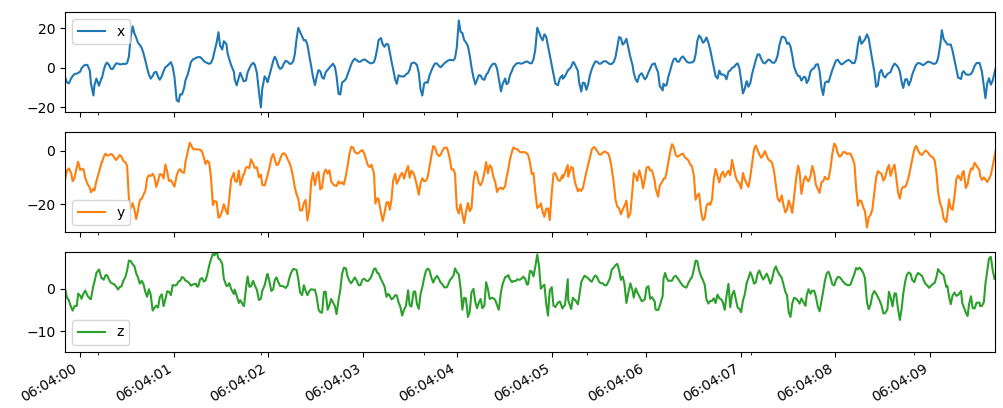
\includegraphics[width=.9\textwidth]{rope_skipping/jump_slow_pols (10 sec).PNG}
\end{figure}

Door de smartwatch aan een andere pols te dragen worden de x- en y-as omgekeerd. Ook zullen ze onder een iets andere hoek komen te staan. De z-component zal alleen onder een andere hoek komen te staan en niet omkeren. Dit resulteert in andere meetwaarden en dus een ander verloop van het signaal (zie Figuur \ref{fig:anderepols}).

\subsection{Draairichting}
\begin{figure}[!htpd]
\centering
\caption{Andere draairichting}\label{fig:anderedraai}
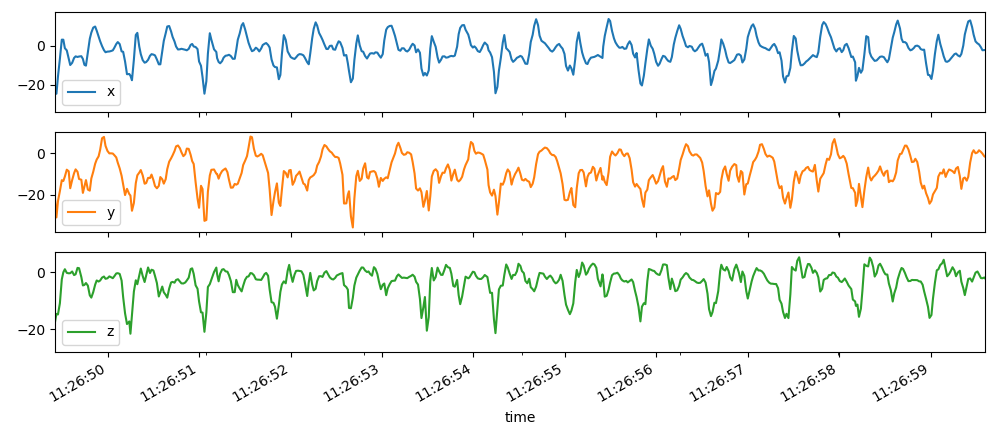
\includegraphics[width=.9\textwidth]{rope_skipping/jump_slow_turn (10 sec).PNG} 
\end{figure}

Een andere draairichting zal de versnellingsvector zelf omkeren terwijl de assen gelijk blijven. Ook hier is er sprake van een gewijzigd verloop van het signaal (zie Figuur \ref{fig:anderedraai}).

\section{Selectie machine learning algoritme}
Machine learning is een modeling techniek gebaseerd op data. Het systeem heeft als input een training set waaruit het model afgeleid wordt. Diversiteit van de training dataset is belangrijk. Een training dataset bestaande uit enkel geschreven nota's van één persoon zal de cijfers/letters van een ander handschrift bijvoorbeeld niet herkennen. Ook is veralgemening van belang. Dit is het proces waarmee de performantie van een model constant gemaakt wordt onafhankelijk van de training of field dataset. Het model zal bijgevolg ook input herkennen die niet volledig overeenkomt met de data waarop getraind werd. 
Er zijn verschillende types machine learning: supervised learning, unsupervised learning en reinforcement learning. Het herkennen van rope skipping bewegingen valt onder supervised learning. Deze techniek zal vanuit een leerverzameling getraind worden om data te herkennen.

Het is belangrijk om het bekomen model correct te evalueren. Zo is geweten of nog meer data of verdere tuning nodig is. Er wordt een score gegeven aan het model waarvoor verschillende metrieken bestaan.
\textit{Accuracy} is het ratio van correct geclassificeerde datapunten en het totaal aantal datapunten. 
\textit{Recall} is het ratio van het totaal aantal correct geclassificeerde positieve samples en het totaal aantal positieve samples. Een positief geclassificeerd datapunt (\textit{true positive}) is een datapunt dat wordt bestempeld met het juiste label. 
\textit{Precision} is het ratio van het aantal correct geclassificeerde positieve samples en het totaal aantal voorspelde positieve samples.
De F1 score is een samensmelting van de recall en precision scores.

Vergelijken van machine learning algoritmes wordt gedaan met confusion matrices. Deze matrices geven een beeld van het aantal \textit{true positives/negatives} en \textit{false positives/negatives}. 

Voor de implementatie van de algoritmes werd grotendeels Scikit Learn gebruikt. Enkel het \textit{convolutional neural network} is afkomstig uit Tensorflow \citep{ref3} \cite{ref29} \cite{ref30}.

In een eerste fase werd het meest optimale model gezocht. Via train test split werd in deze fase een training en test dataset bekomen. Alle modellen naast CNN vereisen meer input dan enkel accelerometer data. Hierdoor werd een groot aantal dimensies bekomen. Deze werden via dimensionality reduction gereduceerd naar 6. In wat volgt wordt de werking van de algoritmen en de resultaten ervan kort besproken. Er werd telkens gebruik gemaakt van \textit{gridSearch} om de meest optimale hyperparameters te bepalen. Het gridSearch algoritme zal namelijk elke combinatie van hyperparameters uitvoeren en degene met de beste accuraatheid teruggeven. Hier werd een window van 1 seconde gebruikt met telkens 50\% overlap.

\subsection{Support Vector Classification}
SVM zorgt voor het maken van een \textit{decision boundary} tussen de verschillende klassen.
In het geval van lineaire scheiding moet ervoor gezorgd worden dat de afstand tussen de boundary en het dichtstbijzijnde datapunt zo groot mogelijk is. Deze decision boundary is een \textit{hyperplane} in een n-dimensionale ruimte waarbij n het aantal features zijn die een datapunt beschrijven. Het hyperplane heeft telkens een dimensie van n-1. Er bestaan veel zulke hyperplanes maar hiervan moet degene gekozen worden met maximale marge.
Bij non-lineaire gevallen wordt gebruik gemaakt van twee concepten: \textit{soft margin} en \textit{kernel tricks}. 
Soft margin wil zeggen dat er een hyperplane gekozen wordt met een aantal verkeerd geclassificeerde datapunten. Hierbij worden twee soorten misclassificaties getolereerd. Een datapunt bevindt zich aan de verkeerde kant van het hyperplane maar wel nog binnen de marge of het datapunt bevindt zich aan de verkeerde kant van het hyperplane en niet binnen de marge. SVM zal dus de balans moeten vinden tussen maximale marge en minimaal misgeclassificeerde datapunten. De hoeveelheid tolerantie die gekozen wordt is een belangrijke hyperparameter. Deze wordt voorgesteld door C in Scikit Learn. Hoe groter C, hoe meer \textit{penalty} het model krijgt bij misclassificatie. De marge zal bij grote C kleiner zijn en er zullen minder \textit{support vectors} zijn. Bij \textit{noisy} data is het dus beter om C niet al te groot te nemen.
Een belangrijk concept hierbij zijn de support vectors. Dit zijn datapunten dichtst bij het hyperplane. De afstand tussen deze vectors moet bijgevolg maximaal gemaakt worden.
De kernel wordt gebruikt om datapunten te herschalen naar een grotere dimensionale ruimte waarin het mogelijk is om de punten met een hyperplane te scheiden. Zo wordt een non-lineaire decision boundary gevonden.
De loss functie, ook wel cost functie genoemd, zal aan elke classificatie een kost toewijzen. 
Door de afgeleide te nemen van deze functie kan gevonden worden in welke richting de gewichten moeten aangepast worden. De gewichten zijn de coördinaten van een vector die loodrecht op het hyperplane staat.
Een regularisatie term kan toegevoegd worden aan de loss functie, deze zal de mate waarin loss wordt toegewezen aan verkeerd geclassificeerde datapunten aanpassen. Op die manier kan overfitting voorkomen worden.

SVC implementeert het \textit{one-against-one} algoritme voor \textit{multiclass classification}. \textit{Classifiers} worden aangemaakt die elk data van 2 klassen trainen. Er zijn dus  n\_class * (n\_class-1)/2 classifiers nodig \cite{ref31}.

De resultaten na toepassing van dit algoritme op de dataset zijn te zien in Figuur \ref{fig:SVC} en Tabel \ref{tab:svc_precision_recall}. Bepaalde klassen worden zeer slecht herkend, andere matig.

\begin{figure}[!htpd]
\centering
\caption{Confusion matrix van SVC}\label{fig:SVC}
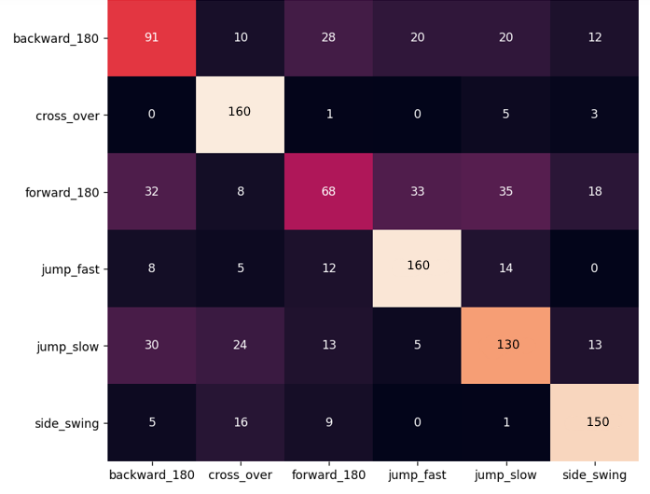
\includegraphics[width=.9\textwidth]{rope_skipping/confusion_matrix_SVC.PNG} 
\end{figure}

\begin{table}[!htpd]
  \centering
  \caption{Precision en recall van SVC}
  \label{tab:svc_precision_recall}
\begin{tabular}{lccc}
 \hline \\
\textbf{}             & \textbf{Precision} & \textbf{Recall} & \textbf{F1} &  \\
\hline \\
\textbf{Forward 180}  & 0.52               & 0.35            & 0.42 & \\
\textbf{Backward 180} & 0.55               & 0.50            & 0.52 & \\
\textbf{Jump slow}    & 0.63               & 0.60            & 0.61 & \\
\textbf{Jump fast}    & 0.74               & 0.80            & 0.77 & \\
\textbf{Cross over}   & 0.72               & 0.95            & 0.82 & \\
\textbf{Side swing}   & 0.77               & 0.83            & 0.80 \\ \\
\hline \\
\end{tabular}
\end{table}

\subsection{Linear Support Vector Classification}

Dit algoritme is vergelijkbaar met SVC indien voor de parameter kernel linear gekozen wordt. Het heeft echter meer flexibiliteit bij het kiezen van penalties en loss functies en zou beter moeten schalen naar grote aantallen samples. 
Support Vector Classifiation doet zijn classificatie, net zoals SVC, door een hyperplane te creëren die de data scheidt in klassen. Hierbij moet de afstand met de support vectors (dit zijn datapunten dichtst bij het hyperplane) maximaal gemaakt worden.
De kernel wordt gebruikt om datapunten te herschalen naar een grotere dimensionale ruimte waarin het mogelijk is om de punten met een hyperplane te scheiden. Zo wordt een non-lineaire descision boundary gevonden. LinearSVC gebruikt een lineaire kernel en vindt dus enkel lineaire decision boundaries.

LinearSVC implementeert de \textit{one-vs-the-rest multiclass} strategie, wat trainen van n\_class modellen betekent. Met optie multi\_class wordt een andere multiclass strategie geselecteerd. Het is echter aangewezen om one-vs-rest te gebruiken aangezien dit algoritme veel sneller is \cite{ref32} \cite{ref33} \cite{ref34}.

De resultaten bekomen na toepassing van linearSVC zijn te zien op Figuur \ref{fig:linearSVC} en Tabel \ref{tab:linearsvc_precision_recall}. De slechtere performantie van dit algoritme was te verwachten aangezien het onderzochte classificatie probleem hoogstwaarschijnlijk niet lineair scheidbaar is.

\begin{figure}[!htpd]
\centering
\caption{Confusion matrix van linearSVC}\label{fig:linearSVC}
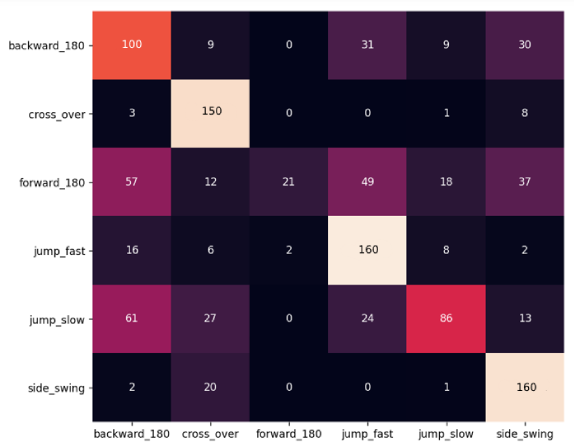
\includegraphics[width=.9\textwidth]{rope_skipping/confusion_matrix_LinearSVC.PNG}  
\end{figure}

\begin{table}[!htpd]
  \centering
  \caption{Precision en recall van linearSVC}
  \label{tab:linearsvc_precision_recall}
\begin{tabular}{lccc}
 \hline \\
\textbf{}             & \textbf{Precision} & \textbf{Recall} & \textbf{F1} &  \\
\hline \\
\textbf{Forward 180}  & 0.91               & 0.11            & 0.20 & \\
\textbf{Backward 180} & 0.42               & 0.56            & 0.48 & \\
\textbf{Jump slow}    & 0.70               & 0.41            & 0.52 & \\
\textbf{Jump fast}    & 0.61               & 0.82            & 0.70 & \\
\textbf{Cross over}   & 0.67               & 0.93            & 0.78 & \\
\textbf{Side swing}   & 0.64               & 0.87            & 0.74 \\ \\
\hline \\
\end{tabular}
\end{table}

\subsection{Random Forest Classifier}
Beslissingsbomen zijn de bouwstenen van het Random Forest model, deze bomen zullen vertakkingen opbouwen aan de hand van features. Er zijn evenveel takken als er mogelijkheden zijn voor waarden van die feature. Random Forest bestaat uit verschillende beslissingsbomen die samenwerken. Elke beslissingsboom in het forest zal een predictie doen. De klasse die het meest voorkomt bij deze predicties wordt de definitieve voorspelling van het model. Er mag geen of geen grote correlatie zijn tussen de verschillende beslissingsbomen. Is dit wel zo dan wordt de kracht van het forest teniet gedaan aangezien het zich nu zal gedragen als één geheel. De verschillende bomen vangen namelijk hun individuele fouten op. Beslissingsbomen zijn zeer gevoelig voor de data waarop ze getraind hebben. Een kleine wijziging hieraan resulteert al in zeer verschillende bomen. Elke boom zal random sampelen met vervanging, hierdoor is de training data van elke boom anders. \textit{Feature randomness} doet zich voor door een proces genaamd \textit{bagging}. Elke boom neemt, bij splitsing van een knoop, de feature die voor het meeste onderscheid zorgt. Dit zal dus ook sterk verschillen tussen bomen.
De belangrijkste hyperparameters zijn de volgende:
Max features geeft de random subset van features weer. Hoe lager dit getal, hoe meer vermindering in variantie en ook hoe meer bias. 
N\_estimators stelt het aantal trees in het bos voor. Naarmate het aantal bomen toeneemt, neemt over het algemeen de fout tot een bepaald punt af. De nauwkeurigheid neemt vanaf dat punt niet meer toe. 
Max\_depth geeft de maximale diepte van iedere boom in het forest aan. Hoe dieper een boom is, hoe meer hoe meer splitsingen er gebeurd zijn en hoe meer informatie over de data aanwezig is.
Min\_samples\_split is het minimum aantal datapunten die nodig zijn om een interne node op te splitsen \cite{ref35}.

De resultaten van dit algoritme zijn te zien op Figuur \ref{fig:random_forest} en Tabel \ref{tab:randomForest}. De performantie is gestegen ten opzichte van eerder bekeken algoritmen. Het zijn echter opnieuw dezelfde klassen die minder goed geclassificeerd worden.

\begin{figure}[!htpd]
\centering
\caption{Confusion matrix van Random Forest}\label{fig:random_forest}
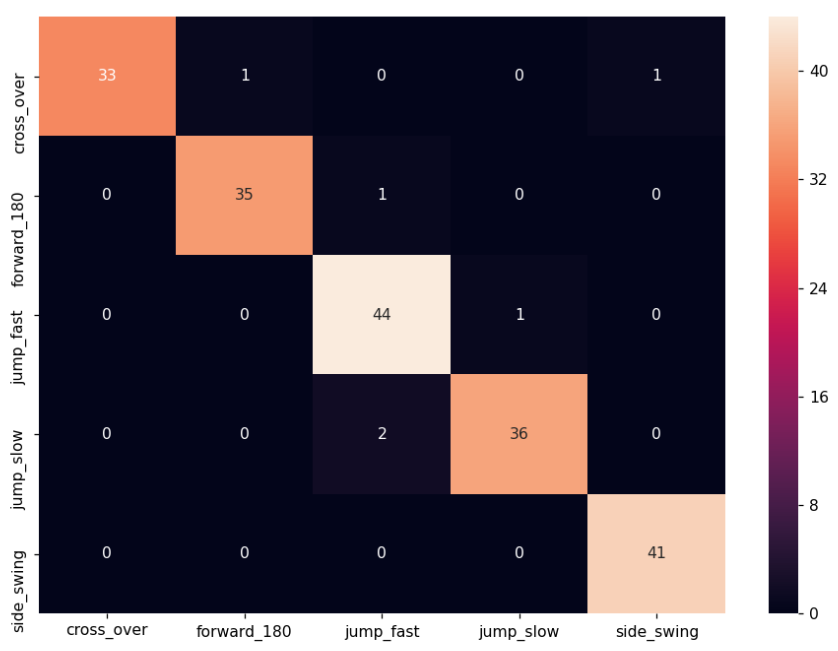
\includegraphics[width=.9\textwidth]{rope_skipping/confusion_matrix_random_forest.PNG}
\end{figure}

\begin{table}[!htpd]
  \centering
  \caption{Precision en recall van Random Forest}
  \label{tab:randomForest}
\begin{tabular}{lccc}
 \hline \\
\textbf{}             & \textbf{Precision} & \textbf{Recall} & \textbf{F1} &  \\
 \hline \\
\textbf{Forward 180}  & 0.63               & 0.53            & 0.58        &  \\
\textbf{Backward 180} & 0.64               & 0.71            & 0.67        &  \\
\textbf{Jump slow}    & 0.68               & 0.68            & 0.68        &  \\
\textbf{Jump fast}    & 0.80               & 0.79            & 0.79        &  \\
\textbf{Cross over}   & 0.82               & 0.90            & 0.86        &  \\
\textbf{Side swing}   & 0.88               & 0.88            & 0.88        & \\ \\
 \hline \\
\end{tabular}
\end{table}

\subsection{AdaBoost}
Adaboost combineert verschillende zwakke classifiers, die slechts lichtjes beter zijn dan \textit{random guessing}, in één sterke classifier. Elke zwakke classifier wordt getraind op een subset van de totale trainingsdata. Deze subsets mogen hierbij overlappen. Elk datapunt krijgt een gewicht toegewezen. Samples met een hoger gewicht hebben meer kans om gekozen te worden. Na training zal Adaboost het gewicht van misgeclassificeerde samples verhogen. Op die manier kan meer aandacht hieraan besteed worden tijdens de volgende iteratie. Classifiers met grotere accuraatheid krijgen meer gewicht. Door de resultaten en gewichten van alle classifiers in rekening te brengen, wordt het Adaboost model bekomen. 

Hoe de zwakke learners geïmplementeerd worden in Adaboost is afhankelijk van hyperparameter base\_estimator. Vaak worden echter beslissingsbomen met één vertakkingsgraad (\textit{decision stumps}) gebruikt. Decision stumps splitsen de dataset in twee gebaseerd op één feature aan de hand van een threshold.

De implementatie in Scikit Learn kan geoptimaliseerd worden met de volgende hyperparameters. Het aantal zwakke learners kan aangegeven worden met de n\_estimators parameter. Hoe meer er van deze aanwezig zijn, hoe complexer de decision boundary is.
De learning rate zwakt de contributie van opeenvolgende iteraties af met een vooraf gedefinieerde factor. Op die manier zal de classifier minder snel leren \cite{ref36}.

Figuur \ref{fig:adaboost} en Tabel \ref{tab:adaboost} geven de resultaten van dit experiment weer. Dit algoritme heeft een gelijkaardige performantie als Random Forest.

\begin{figure}[!htpd]
\centering
\caption{Confusion matrix van Adaboost}\label{fig:adaboost}
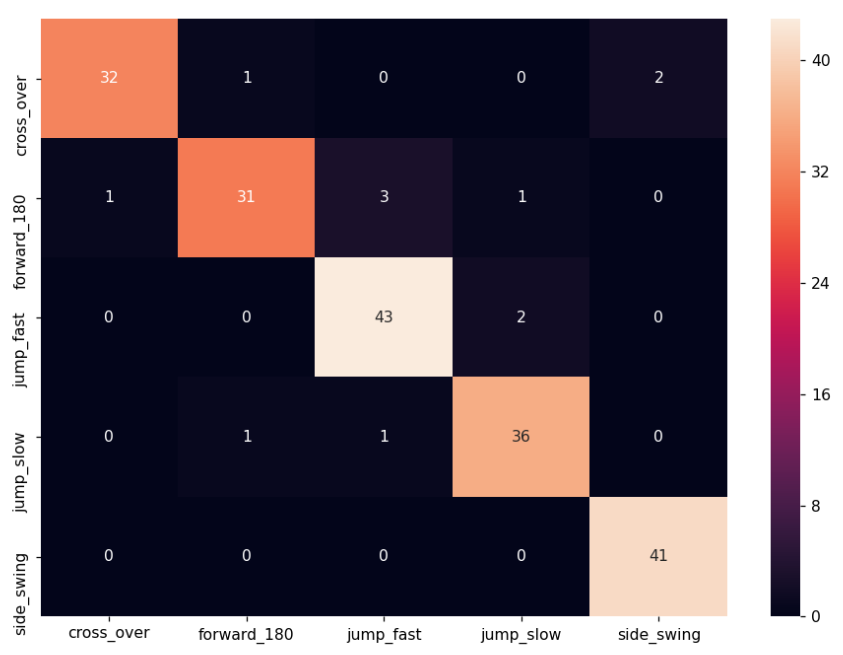
\includegraphics[width=.9\textwidth]{rope_skipping/confusion_matrix_Adaboost.PNG} 
\end{figure}

\begin{table}[!htpd]
  \centering
  \caption{Precision en recall van Adaboost}
  \label{tab:adaboost}
\begin{tabular}{lccc}
 \hline \\
\textbf{}             & \textbf{Precision} & \textbf{Recall} & \textbf{F1} &  \\
\hline \\
\textbf{Forward 180}  & 0.67               & 0.55            & 0.60        &  \\
\textbf{Backward 180} & 0.64               & 0.68            & 0.66        &  \\
\textbf{Jump slow}    & 0.67               & 0.74            & 0.70        &  \\
\textbf{Jump fast}    & 0.79               & 0.77            & 0.78        &  \\
\textbf{Cross over}   & 0.84               & 0.91            & 0.87        &  \\
\textbf{Side swing}   & 0.93               & 0.88            & 0.90        & \\\\
\hline \\
\end{tabular}
\end{table}

\subsection{Naive Bayes}
Naive Bayes is gebaseerd op de Bayes theorie waarbij verondersteld wordt dat de features niet gecorreleerd zijn. 
Naive Bayes berekent de kans dat een feature een bepaalde waarde heeft, gebaseerd op de waarde van een andere feature. 
De klasse met de grootste \textit{posterior probability} is de uiteindelijke voorspelling voor het datapunt. 
Voor elke klasse wordt bijgevolg de kans P(c|f), waarbij c de klasse voorstelt, berekend en dit met elke mogelijke waarde van feature f. 
Naive Bayes is een simpel algoritme dat grote voordelen heeft. 
Er is weinig training data nodig om zeer snel goede resultaten af te leveren. Doordat Naive Bayes geen correlatie veronderstelt tussen de k features moet er geen rekening gehouden worden met de \(2^k\) mogelijke feature interacties.
Hierdoor is Naive Bayes sneller en even performant met kleine datasets in vergelijking met een complex neuraal netwerk. 
Het algoritme presteert goed met categorische variabelen aangezien voor elke waarde van een feature een berekening moet uitgevoerd worden waardoor dit belastend kan zijn in geval van continue variabelen. 
Een ongeziene categorische variabele zal het model echter niet kunnen voorspellen aangezien deze waarden een probabiliteit heeft van 0. 
Er wordt verondersteld dat de features onafhankelijk van elkaar zijn, wat in de praktijk vaak niet zo is.

Parameter alpha geeft aan hoeveel \textit{smoothing} moet toegepast worden op de berekening van de posterior probability. Dit zorgt ervoor dat deze kan nooit nul kan worden \cite{ref37} \cite{ref38}.

Figuur \ref{fig:naive_bayes} en Tabel \ref{tab:naivebayes} visualiseren de resultaten. Deze resultaten laten aan de wensen over vanwege de gebruikte dataset. De vectoren bestaan namelijk uit continue variabelen. Ook is de veronderstelling dat er geen correlatie aanwezig is tussen de features onderling incorrect.

\begin{figure}[!htpd]
\centering
\caption{Confusion matrix van Naive Bayes}\label{fig:naive_bayes}
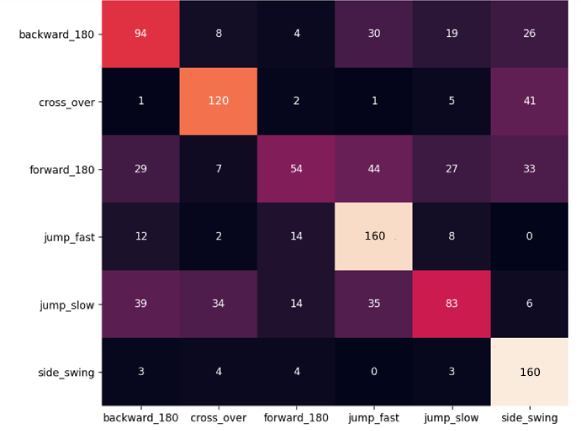
\includegraphics[width=.9\textwidth]{rope_skipping/confusion_matrix_naiveBayes.PNG}  
\end{figure}

\begin{table}[!htpd]
  \centering
  \caption{Precision en recall van Naive Bayes}
  \label{tab:naivebayes}
\begin{tabular}{lccc}
 \hline \\
\textbf{}             & \textbf{Precision} & \textbf{Recall} & \textbf{F1} &  \\
\hline \\
\textbf{Forward 180}  & 0.59               & 0.28            & 0.38        &  \\
\textbf{Backward 180} & 0.53               & 0.52            & 0.52        &  \\
\textbf{Jump slow}    & 0.57               & 0.39            & 0.46        &  \\
\textbf{Jump fast}    & 0.59               & 0.82            & 0.69        &  \\
\textbf{Cross over}   & 0.69               & 0.71            & 0.70        &  \\
\textbf{Side swing}   & 0.60               & 0.92            & 0.73        & \\\\
\hline \\
\end{tabular}
\end{table}

\subsection{K-nearest neighbors}
K-nearest neighbors gaat ervan uit dat gelijkaardige zaken zich in elkaars buurt bevinden. Het algoritme berekent de afstand tussen datapunten gebruikmakend van een bepaalde afstandsmetriek. De euclidische afstand is hierbij de meest voorkomende. 
Het algoritme werkt als volgt: voor elk datapunt wordt de afstand berekend tot alle andere datapunten. Deze afstanden worden vervolgens gesorteerd. 
De meest voorkomende klasse van de k datapunten met de kleinste afstand wordt als voorspelling teruggegeven. 
K is hier de enige en dus ook belangrijkste hyperparameter. 

Dit simpel algoritme heeft zo zijn voordelen. 
Er is slechts één hyperparameter waardoor geen tijd verloren gaat aan het \textit{tunen} van vele parameters. Ook is het bouwen van een complex model niet nodig. 
Bij grote datasets is KNN echter minder performant.

Belangrijke parameters in de Scikit Learn implementatie zijn n\_neighbors, weights, algorithm, leaf\_size en metric.
n\_neighbors stelt k voor. Deze parameter kan een waarde hebben tussen 1 en n-1, waarbij n het aantal datapunten is in de dataset. Een kleine waarde kiezen voor k kan soms onstabiele resultaten geven. Stel dat een datapunt omringd wordt door datapunten van bijna exclusief één bepaalde klasse met slechts een klein aantal behorende tot een tweede verschillende klasse. Liggen de datapunten van deze minder voorkomende klasse toevallig dichterbij dan de rest, dan kan het resultaat met kleine k een vertekend beeld gegeven worden.
Maken we k te groot dan is het mogelijk dat meer misclassificaties ontstaan aangezien ook verder liggende punten in rekening worden gebracht. Een grote k is echter wel in staat om ruis te onderdrukken.
K is best een oneven nummer om geen ex-aequos te vormen.

De weights parameter kan ingesteld worden op uniform of distance. Uniform zal aan alle datapunten evenveel gewicht toekennen.
De configuratie met distance zal de dichtstbijzijnde punten zwaarder laten doorwegen dan punten op een grotere afstand.

De parameter \textit{algorithm} stelt het gebruikte zoekalgoritme in. Doordat telkens alle samples moeten overlopen worden bij classificatie van een nieuw datapunt, is het nuttig om met een efficiënte datastructuur te werken.
Hiervoor zijn enkele opties. Een KD tree is voordelig bij datasets met grote dimensionaliteit maar met een klein aantal datapunten.
Zoeken in deze structuur verloopt echter trager bij grote k.
Een ball tree is nuttig bij zowel grote dimensionaliteit als groot aantal samples. Ook deze structuur presteert slechter bij grote k.

Er kan voor gekozen worden om bij een bepaald aantal datapunten over te schakelen op het brute force algoritme. Dit wordt ingesteld met behulp van de leaf size parameter.

Als laatste kan de gebruikte afstandsmetriek meegegeven worden met behulp van de parameter metric \cite{ref39}.

De resultaten van dit experiment zijn te zien op Figuur \ref{fig:kneighbors} en \ref{tab:kneighbors}. Het is duidelijk dat ook dit algoritme geen match is.

\begin{figure}[!htpd]
\centering
\caption{Confusion matrix van K-nearest neighbors}\label{fig:kneighbors}
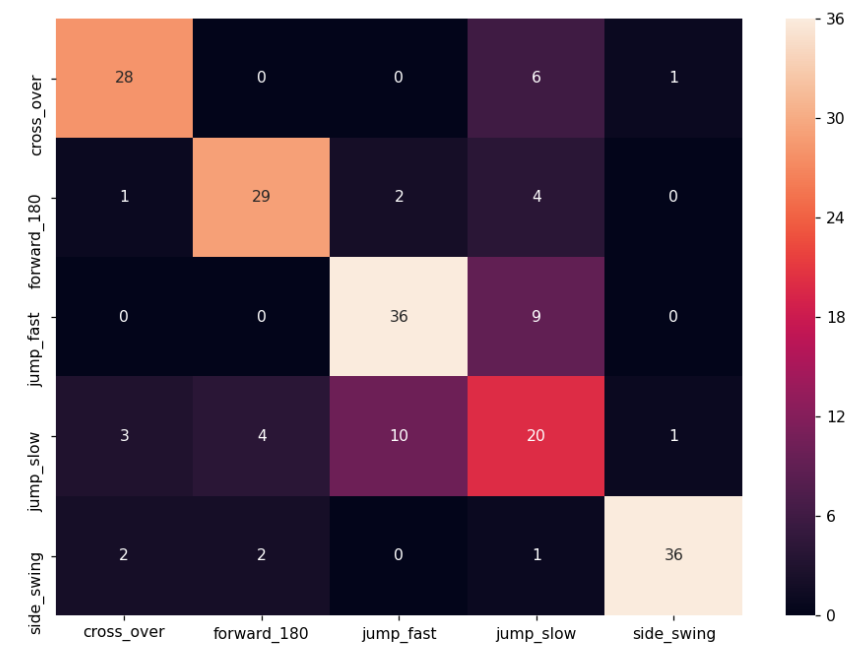
\includegraphics[width=.9\textwidth]{rope_skipping/confusion_matrix_kneighbors.png}   
\end{figure}

\begin{table}[!htpd]
  \centering
  \caption{Precision en recall van K neighbors}
  \label{tab:kneighbors}
\begin{tabular}{lccc}
 \hline \\
\textbf{}             & \textbf{Precision} & \textbf{Recall} & \textbf{F1} &  \\
\hline \\
\textbf{Forward 180}  & 0.38               & 0.30            & 0.34        &  \\
\textbf{Backward 180} & 0.45               & 0.52            & 0.48        &  \\
\textbf{Jump slow}    & 0.51               & 0.34            & 0.41        &  \\
\textbf{Jump fast}    & 0.71               & 0.77            & 0.74        &  \\
\textbf{Cross over}   & 0.71               & 0.88            & 0.79        &  \\
\textbf{Side swing}   & 0.71               & 0.83            & 0.77        & \\\\
\hline \\
\end{tabular}
\end{table}

\subsection{Stochastic Gradient Descent classifier}
De decision boundary wordt, in geval van SGD, voorgesteld door een vector loodrecht op het hyperplane. Door de gewichten van deze vector aan te passen kan de positie van deze boundary veranderd worden. Dit om een optimale classificatie te bekomen. 
Aan de hand van een loss functie wordt berekend wat de totale loss van het model is. Bij misclassificatie wordt aan een datapunt een kost toegekend. De loss functie bepaalt hoe groot deze kost is. Door deze functie dus minimaal te maken kan de meest optimale decision boundary gevonden worden. 
Door de afgeleide te berekenen ten op zichtte van elke feature wordt gekeken in welke richting het hyperplane, in die dimensie, moeten aangepast worden om de minimale kost te bereiken. 
Via een parameter alpha wordt de learning rate meegegeven. Dit geeft aan hoe groot de stappen zijn bij elke update van parameters.
Stochastic gradient descent berekent een benadering voor de gradiënt aan de hand van slechts één datapunt. Dit is efficiënter dan alle datapunten hiervoor te overlopen en pas dan een update door te voeren. Voor grote datasets is dit een zeer goede oplossing. 
De gewichten van het model worden aangepast overeenstemmend met de berekende gradiënt in dat datapunt. 

SGD maakt gebruik van randomness, de training data wordt dus best geshuffeld voor fitting.
Ook wordt de data best geschaald aangezien datapunten met elkaar moeten vergeleken worden.

belangrijke tuning parameters bij dit algoritme zijn alpha, learning rate en max\_iter.
Zoals eerder vermeld geeft alpha weer hoe groot de stappen zijn bij elke update van de model parameters.
Alpha is dus een getal tussen 0 en 1 waarbij een waarde van 1 betekent dat de update totaal niet wordt afgezwakt. 0 betekent dat er geen updates worden doorgevoerd.
Een te grote alpha zorgt ervoor dat het model te snel convergeert naar een niet optimale toestand.
Een te kleine alpha kan ervoor zorgen dat het learning proces vast komt te zitten.

Met de parameter learning rate wordt het \textit{learning rate schedule} bepaald. Het soort schedule geeft weer hoe de learning rate verandert in de tijd.

Het maximum aantal iteraties hangt gedeeltelijk samen met alpha. Bij een kleine learning rate zijn ook meer iteraties nodig \cite{ref40} \cite{ref41} \cite{ref42}.

De resultaten zijn ook hier te zien op Figuur \ref{fig:SGD} en Tabel \ref{tab:SGD}. Deze performantie ligt in lijn met de resultaten bekomen door K-nearest neighbors.

\begin{figure}[!htpd]
\centering
\caption{Confusion matrix van Stochastic Gradient Descent}\label{fig:SGD}
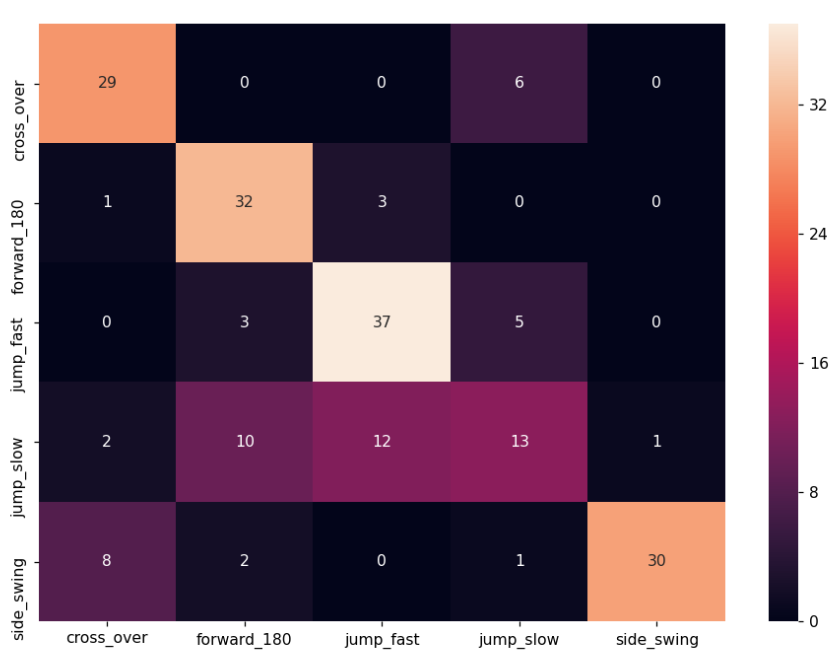
\includegraphics[width=.9\textwidth]{rope_skipping/confusion_matrix_SGD.PNG}  
\end{figure}

\begin{table}[!htpd]
  \centering
  \caption{Precision en recall van SGD}
  \label{tab:SGD}
\begin{tabular}{lccc}
 \hline \\
\textbf{}             & \textbf{Precision} & \textbf{Recall} & \textbf{F1} &  \\
\hline \\
\textbf{Forward 180}  & 0.56               & 0.12            & 0.20        &  \\
\textbf{Backward 180} & 0.46               & 0.48            & 0.47        &  \\
\textbf{Jump slow}    & 0.62               & 0.42            & 0.50        &  \\
\textbf{Jump fast}    & 0.60               & 0.85            & 0.70        &  \\
\textbf{Cross over}   & 0.67               & 0.89            & 0.76        &  \\
\textbf{Side swing}   & 0.59               & 0.86            & 0.70        & \\\\
\hline \\
\end{tabular}
\end{table}

\subsection{Multilayer Perceptron classifier}

MLP is één van de gemakkelijkst te implementeren neurale netwerken.
Een perceptron is de kleinste eenheid van zo'n neuraal netwerk. Dit element zal een aantal inputs met hun corresponderende gewichten vermenigvuldigen en hierbij een bias optellen. Via een activatie functie wordt de output bekomen van de perceptron. Een \textit{multilayer perceptron} bestaat uit minstens drie \textit{nodes} waarvan elk, naast de input node, een non-lineaire activatie functie gebruikt. De nodes tussen de input en output node worden ondergebracht in lagen, \textit{hidden layers} genoemd.

Een loss functie meet de performantie van het netwerk. Een hoge loss betekent dat de voorspelde klasse voor veel datapunten niet correct is. Het is de bedoeling om een set gewichten te vinden die deze loss functie minimaliseert. Het is echter mogelijk dat er meerdere lokale minima voorkomen, verschillende gewicht initialisaties kunnen dus andere resultaten hebben.
De activiatiefunctie beschrijft een non-lineaire relatie tussen input en output. Populaire functies zijn Sigmoid, Relu en Tanh. Het trainen van het model gebeurt in drie fasen: \textit{forward pass, loss calculation} en \textit{backward pass}. Bij de forward pass wordt de input via de lagen doorgegeven waarna uiteindelijk een output wordt berekend. Vervolgens komt een eerste berekening van de loss. Door de partiële afgeleiden te nemen van de loss functie met betrekking tot de verschillende parameters worden de gewichten aangepast (backward pass). In elke laag moet de node die de meeste fouten veroorzaakt heeft beboet worden door hieraan een kleiner gewicht te koppelen.
Muliticlass classificatie wordt mogelijk gemaakt door als laatste laag een Softmax functie te gebruiken.
Een voordeel van deze classifier is de mogelijkheid tot een non-lineaire decision boundary.
Een nadeel is echter dat de loss functie convex is en meer dan één lokaal minimum bevat. Er is eveneens sprake van een grote hoeveelheid hyperparameters. 

Een aantal van de belangrijkste hyperparameters zijn: de gekozen activation functie, alpha en hidden\_layer\_sizes. Alpha stelt de mate van regularisatie in. De hoeveelheid regularisatie bepaalt in welke mate misgeclassificeerde datapunten toegelaten worden.
Met de parameter hidden layer sizes wordt bepaalt van hoeveel hidden layers gebruik gemaakt wordt en hoeveel neuronen in elke laag zitten. Het aantal hidden layers is zeer afhankelijk van de inputdata. Indien deze lineair afscheidbaar is, dan zijn zelfs geen hidden layers nodig \cite{ref43} \cite{ref44} \cite{ref45} \cite{ref46}.

De resultaten na toepassing van dit algoritmen zijn zichtbaar op Figuur \ref{fig:MLP} en Tabel \ref{tab:MLP}. De performantie is iets beter dan K-nearest neighbors, maar kan nog niet tippen aan Random Forest en Adaboost.

\begin{figure}[!htpd]
\centering
\caption{Confusion matrix van Multilayer Perceptron classifier}\label{fig:MLP}
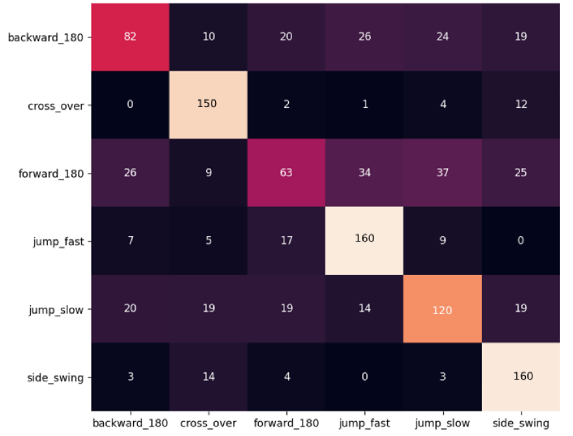
\includegraphics[width=.9\textwidth]{rope_skipping/confusion_matrix_MLP.PNG} 
\end{figure}

\begin{table}[!htpd]
  \centering
  \caption{Precision en recall van MLP}
  \label{tab:MLP}
\begin{tabular}{lccc}
 \hline \\
\textbf{}             & \textbf{Precision} & \textbf{Recall} & \textbf{F1} &  \\
\hline \\
\textbf{Forward 180}  & 0.50               & 0.32            & 0.39        &  \\
\textbf{Backward 180} & 0.59               & 0.45            & 0.51        &  \\
\textbf{Jump slow}    & 0.61               & 0.57            & 0.59        &  \\
\textbf{Jump fast}    & 0.68               & 0.81            & 0.74        &  \\
\textbf{Cross over}   & 0.72               & 0.89            & 0.80        &  \\
\textbf{Side swing}   & 0.68               & 0.87            & 0.76        & \\\\
\hline \\
\end{tabular}
\end{table}

\subsection{CNN} \label{subsectie:cnn}
Dit soort netwerk wordt gekenmerkt door de Convolutional Layer en onderscheidt zich hierdoor van MLP.

Deep learning imiteert de werking van het menselijke brein in de manier van processen van data en maken van patronen voor gebruik in beslissingen. Het is een subset van machine learning en gebruikt hiërarchische levels van artificiële neurale netwerken. Data wordt geprocessed op een niet lineaire manier.
CNN wordt vooral gebruikt bij image processing. In dit geval zijn er veel inputs namelijk het totaal aantal pixels. Voor dit soort problemen kan MLP niet gebruikt worden aangezien voor elke input één perceptron voorzien is wat bij veel data niet echt efficiënt is \citep{ref2}. Het algoritme is echter eveneens toepasbaar op bewegingsherkenning.

Zoals eerder vermeld, is de Convolutional Layer de bouwsteen van een CNN. Convolutie gaat een filter laten glijden over de input array en telkens de convolutie nemen van de overdekte oppervlakte. De convolution layer bestaan uit een aantal afzonderlijke filters.
Het doel hiervan is om features te extraheren. De matrix gevormd door de convolutie uit te voeren met de filter en het dot product te berekenen met de gewichten wordt de activation map of feature map genoemd.

De Pooling Layer is een tweede bouwsteen van CNN. Hiermee wordt de grootte van de representatie gereduceerd aangezien dit resulteert in minder parameters en dus minder rekenwerk. Dit kan aanzien worden als een soort dimensionality reduction. Max pooling, één van de pooling technieken, wordt het meest gebruikt. Hierbij wordt een oppervlak bekeken waaruit enkel de maximum waarde behouden wordt. Door het aantal parameters te reduceren wordt overfitting voorkomen. Dit proces maakt het netwerk eveneens robuust tegen kleine variaties in input data.

Een andere veel gebruikte laag is Relu. Dit is een non-lineaire operatie. De data die het model moet leren zal hoogstwaarschijnlijk non-lineair zijn daarom is het introduceren van non-lineariteit noodzakelijk. Er bestaan ook andere non-lineaire operatie (Tanh en Sigmoid). Relu geeft echter betere resultaten.

Een Fully Connected Layer is een traditionele MLP laag met een Softmax activatie functie in de output layer. Fully connected wil zeggen dat elk neuron uit de vorige laag geconnecteerd is met elke neuron in de laag die erop volgt.
Deze geconnecteerde laag gebruikt de high level features bekomen uit de pooling en convolutie lagen met als doel deze te classificeren. 

In eerste instantie worden de filters en gewichten random geïnitialiseerd. Na de \textit{forward propagation} fase wordt de loss van het model berekend. De gewichten worden geüpdatet door de gradiënt ten opzichte van elke parameter te berekenen. Zo is geweten in welke richting deze moet aangepast worden. In de \textit{backward propagation} fase worden de gewichten effectief ge-update \cite{ref47} \cite{ref48}.

Om overfitting te voorkomen kan gebruik gemaakt worden van een Dropout laag. Deze laag zal bij iedere iteratie een vooraf opgegeven aantal neuronen negeren \cite{ref49}.

Doordat de \textit{input shape} telkens gelijk moet zijn, kan hier niet gewerkt worden met een variërende segmentgrootte. Hierdoor wordt dit gelijkgesteld aan een gemiddelde waarde van 52 samples.

De resultaten van CNN zijn te zien op Figuur \ref{fig:CNN} en Tabel \ref{tab:CNN}. Dit zijn de best bekomen resultaten tot nu toe. Bijgevolg wordt dit algoritme verder geoptimaliseerd.

\begin{figure}[!htpd]
\centering
\caption{Confusion matrix van CNN}\label{fig:CNN}
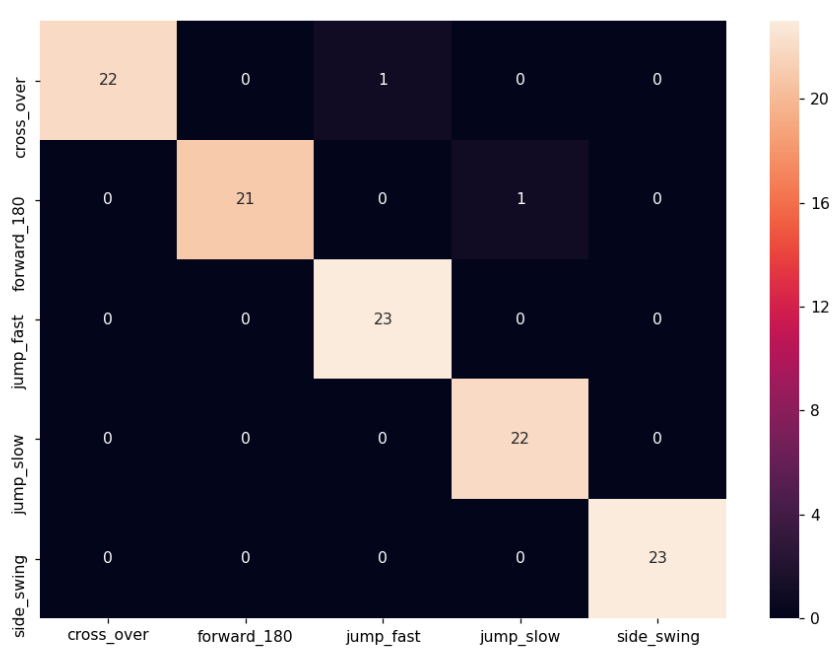
\includegraphics[width=.9\textwidth]{rope_skipping/confusion_matrix_CNN.PNG} 
\end{figure}

\begin{table}[!htpd]
  \centering
  \caption{Precision en recall van CNN}
  \label{tab:CNN}
\begin{tabular}{lccc}
 \hline \\
\textbf{}             & \textbf{Precision} & \textbf{Recall} & \textbf{F1} &  \\
\hline \\
\textbf{Forward 180}  & 0.79               & 0.79            & 0.79        &  \\
\textbf{Backward 180} & 0.86               & 0.86            & 0.86        &  \\
\textbf{Jump slow}    & 0.90               & 0.82            & 0.86        &  \\
\textbf{Jump fast}    & 0.87               & 0.95            & 0.91        &  \\
\textbf{Cross over}   & 0.97               & 1               & 0.98        &  \\
\textbf{Side swing}   & 1                  & 0.96            & 0.98        & \\\\
\hline \\
\end{tabular}
\end{table}

\section{CNN optimalisatie}
Met de klassieke train test split bleek CNN veruit de beste resultaten af te leveren. Dit was in eerste instantie niet zo. Dit kwam echter door een fout in het preprocessen van de data. Voor het maken van segmenten werden de verschillende datapunten geshuffeld. Dit resulteerde in een volledig random model. Wanneer deze fout eruit gehaald werd, werden de resulaten te zien op Figuur \ref{fig:CNN} bekomen. Er werd dus verder gewerkt met dit algoritme. 
Tijdens het trainen van het model werd een callback-functie gebruikt die telkens de beste epoch, deze met de laagste loss, opslaat. Op deze manier wordt steeds het best mogelijke model behouden.
Er werd eveneens besloten om de forward en backward 180 op een andere manier te meten. Oorspronkelijk werd enkel de zuivere beweging gemeten, maar dit is niet realistisch en onnatuurlijk. Tijdens de nieuwe metingen werd een sprong voor de 180 en erna uitgevoerd. Dit is echter ook niet realistisch en zorgde voor meer verwarring in het model. Daarom werd ervoor gekozen om deze beweging niet verder de onderzoeken in het kader van deze thesis.
De redenering achter deze keuze is de volgende. De uiteindelijke gezondheidsapplicatie zal sessies van één bepaalde activiteit aanbevelen. De forward en backward 180 zijn echter bewegingen die moeilijk periodiek kunnen uitgevoerd worden. Ook bleek er grote verwarring tussen backward 180, forward 180 en jump slow onderling. Dit is deels te wijten aan de nieuwe meetwijze dewelke bestaat uit toevoeging van een extra sprong voor en na de backward en forward 180. 
Om het verlies van de forward 180s te compenseren werd gezocht naar een vervangbeweging. De jump run is een goede kandidaat. Uit de vergelijking van de signalen van de jump run, jump slow en jump fast is ook een verschil merkbaar. 

\subsection{validatie dataset}
In een volgend experiment werd een validatie dataset ingevoerd. Deze validatie dataset zal ervoor zorgen dat overfitting van het model voorkomen wordt \cite{ref81}. Tijdens het leerproces zal het netwerk telkens zijn gewichten aanpassen door ook rekening te houden met de validatie data.
Een eerste validatie dataset bestond uit een aantal "scenarios". Tijdens zo'n scenario voert de springer verschillende sprongen door elkaar uit die dan in \textit{postprocessing} geknipt en gelabeld worden.
Het onderscheiden van bepaalde bewegingen in het signaal bleek zeer moeilijk. Om deze reden werd geopteerd voor een validatiedataset bestaande uit periodiek uitgevoerde bewegingen.

\subsection{Window}
Eén van de hyperparameters waaraan kan gesleuteld worden is het window. Tijdens voorgaande experimenten werd standaard gewerkt met een window van één seconde. Dit omdat één enkele sprong steeds een duur heeft van ongeveer één seconde. In Tabel \ref{tab:window} is de accuraatheid ten opzichte van window grootte af te lezen. Deze accuraatheid is een gemiddelde score. Iedere run met een neuraal netwerk levert namelijk verschillende resultaten door de random initialisatie. Aangezien zoals vermeld één sprong een gemiddelde duur van één seconde heeft, is het logisch dat een window van een halve seconde iets minder goede resultaten geeft. Een window groter dan één seconde zal voor problemen zorgen wanneer verschillende bewegingen kort op elkaar volgen. Er zal dan meer dan één beweging aanwezig zijn binnen het window. Om deze reden werd geopteerd voor segmenten van één seconde.

\begin{table}[!htpd]
  \centering
  \caption{Window}
  \label{tab:window}
\begin{tabular}{lccccc}
 \hline \\
\textbf{}         & \textbf{0.5 s} & \textbf{1 s} & \textbf{1.5 s} & \textbf{2 s} & \textbf{3 s} \\
 \hline \\
\textbf{Accuracy} & 0.83           & 0.90         & 0.89           & 0.92         & 0.93  \\\\
 \hline \\
\end{tabular}
\end{table}

\subsection{Overlapping}
Verder werd geëxperimenteerd met al dan niet overlappende segmenten tijdens het trainen. Voorgaande experimenten werkten telkens met 50\% overlap van zowel training en validatie dataset. Een zekere overlapping zal ervoor zorgen dat enerzijds meer trainingsdata ter beschikking is en anderzijds alle karakteristieken van het signaal gemodelleerd worden. Een te grote overlapping zal echter overfitting veroorzaken \cite{ref81}. Dit fenomeen is te zien in Tabel \ref{tab:overlap}. Er werd gekozen om verder te werken met een overlap van 30\%.

\begin{table}[!htpd]
  \centering
  \caption{Overlapping}
  \label{tab:overlap}
\begin{tabular}{lcccc}
 \hline \\
\textbf{}         & \textbf{0\%} & \textbf{30\%} & \textbf{50\%} & \textbf{70\%} \\
\hline \\
\textbf{Accuracy} & 0.88         & 0.93          & 0.90          & 0.93    \\\\
\hline \\
\end{tabular}
\end{table}

\subsection{Splitsen}
Een volgend experiment bestond uit het opsplitsen in meerdere modellen op basis van de variaties in de trainingsdata. Er werden vier modellen getraind, elk gespecialiseerd in één bepaalde soort data. Eén van de model werd getraind op enkel data gemeten aan de rechterpols en in de achterwaartse draairichting, een ander enkel op data gemeten aan de linkerpols en in de achterwaartse draairichting enzovoort. Dit experiment werd inclusief de forward en backward 180 bewegingen uitgevoerd. Deze hebben echter een andere variatie in de vorm van draairichting. Er kan namelijk een draaiing van 180 graden gemaakt worden in twee  richtingen. De accuraatheid steeg hierdoor in de meeste modellen. Er was echter enige verwarring tussen backward en forward 180, wat logisch is aangezien met de nieuwe metingen beide sprongen een jump slow omvatten. 
Met de implementatie van de android applicatie in het achterhoofd werd ervoor gekozen om één model te trainen. In het geval van vier modellen getraind op verschillende data zou de gebruiker telkens moeten opgeven welke variatie men uitvoert (linkerpols-achterwaarts, rechterpols-voorwaarts...). Hierdoor is deze aanpak zeker niet gebruiksvriendelijk.

\subsection{Samenvoegen klassen}
De redenering achter het splitsen van jump slow en jump fast is de volgende. Deze bewegingen vertonen onderling genoeg onderscheid om apart geclassificeerd te worden. Ook steunt de berekening van het aantal draaiingen op dit onderscheid. De gebruikte parameters zijn hierbij verschillend. Bij wijze van experiment werd een samenvoeging van deze klassen uitgevoerd. In Tabel \ref{tab:samenvoegen} is te zien dat dit de classificatie voor het model toch enigszins bemoeilijkt.

\begin{table}[!htpd]
  \centering
  \caption{Samenvoegen jumps}
  \label{tab:samenvoegen}
\begin{tabular}{lccc}
 \hline \\
\textbf{}             & \textbf{Precision} & \textbf{Recall} & \textbf{F1} &  \\
\hline \\
\textbf{Jump run}  & 0.64               & 0.79            & 0.71        &  \\
\textbf{jump}       & 0.97               & 0.87           & 0.92        &  \\
\textbf{Cross over}   & 0.27               & 1               & 0.43        &  \\
\textbf{Side swing}   & 0.79                  & 0.99           & 0.88        & \\\\
\hline \\
\end{tabular}
\end{table}

\subsection{Ensemble learning}
Ensemble learning is een manier om fouten van individuele modellen teniet te doen. Elke nieuwe run van eenzelfde model zal namelijk nooit gelijk zijn met een vorige. Dit door random gewicht initialisaties (zie subsectie \ref{subsectie:cnn}). Vier modellen worden op dezelfde manier getraind met dezelfde input data. Deze modellen zullen samenwerken om tot een oplossing te komen op volgende manier. Wanneer een model een predictie doet, dan wordt aan elk van de klassen een probabiliteit toegekend. Deze probabiliteiten, komende van de vier modellen, worden opgeteld waardoor elk model zijn bijdrage levert tot het uiteindelijke resultaat. De klasse met de hoogste score wordt toegekend aan het segment. Het resultaat hiervan is op Figuur \ref{fig:ensemble} en in Tabel \ref{tab:ensemble} te zien.

\begin{figure}[!htpd]
\centering
\caption{Ensembled model}\label{fig:ensemble}
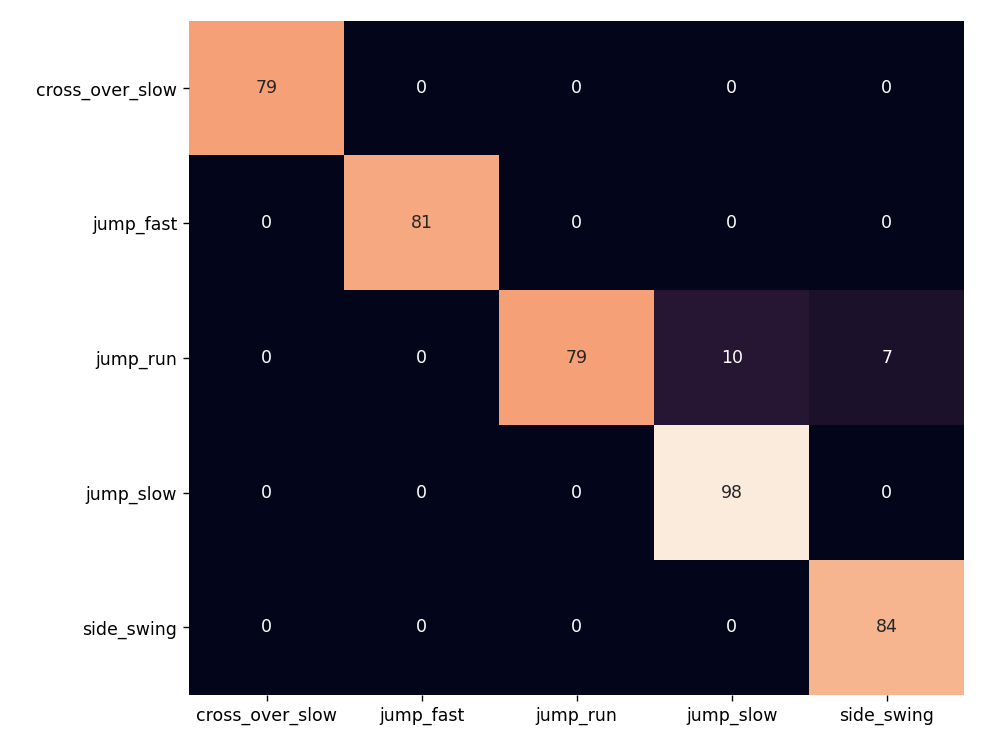
\includegraphics[width=.9\textwidth]{rope_skipping/confusion_matrix_final.PNG} 
\end{figure}

\begin{table}[!htpd]
  \centering
  \caption{Ensembled model performantie}
  \label{tab:ensemble}
\begin{tabular}{lccc}
 \hline \\
\textbf{}             & \textbf{Precision}  & \textbf{Recall}   & \textbf{F1} &  \\
\hline \\
\textbf{Jump run}     & 1                   & 0.82              & 0.90       &  \\
\textbf{Jump slow}    & 0.91                & 1                 & 0.95       &  \\
\textbf{Jump fast}    & 1                   & 1                 & 1       &  \\
\textbf{Cross over}   & 1                   & 1                 & 1        &  \\
\textbf{Side swing}   & 0.92                & 1                 & 0.96       & \\\\
\hline \\
\end{tabular}
\end{table}

\subsection{Lagen}
Deze subsectie licht de gebruikte lagen die eerder al kort beschreven werden toe, toegepast op dit onderzoek. Figuur \ref{fig:lagen} geeft deze lagen weer samen met hun output shape.

\begin{figure}[!htpd]
\centering
\caption{Lagen}\label{fig:lagen}
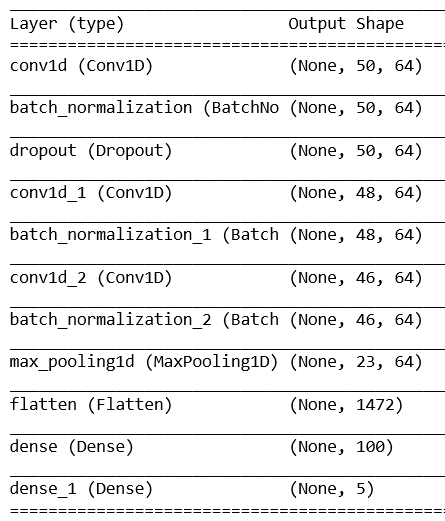
\includegraphics[width=.6\textwidth]{rope_skipping/model_summary.PNG} 
\end{figure}

\subsubsection{Conv1D}
Als eerste wordt gebruik gemaakt van een Conv1D laag. Er werd gekozen voor 1D in plaats van 2D omdat we hier te maken hebben met 1-dimensionale data. Dit is de eerste laag in het model, er moet dus een input\_shape meegegeven worden. De data wordt in segmenten verdeeld met hierin telkens een veelvoud van 52 datapunten, afhankelijk van het gekozen window. 52 Hz is namelijk de gemiddelde frequentie tijdens het datacollectie proces. Elk datapunt bestaat uit 3 dimensies, ook wel \textit{channels} genoemd. De input shape bedraagt bijgevolg (window*52, 3). Er wordt gekozen voor 64 filters. Dit wil zeggen dat de output van deze laag een dimensionality van 64 zal hebben. Als \textit{kernel size} wordt 3 genomen. Dit geeft aan hoe ver de filter zal reiken tijdens het proces van feature extraction en dus in welke mate moet rekening gehouden worden met "context". Ook moet een activatie functie gespecificeerd worden. Ontbreekt deze dan wordt default een lineaire functie gebruikt. Er wordt gekozen voor Relu.
Deze laag wordt meerdere keren toegepast binnen het model, telkens gevolgd door een batchNormalization, aangezien op deze manier meer complexe features kunnen gedetecteerd worden. 

\subsubsection{BatchNormalization}
Vervolgens wordt een BatchNormalization laag ingevoerd. Deze zal ervoor zorgen dat de output van de voorgaande laag genormaliseerd wordt. 
Normalisatie van de trainingsdata is namelijk vereist, maar niet noodzakelijk ten opzichte van ieder afzonderlijk datapunt. Onderstaande Figuren \ref{fig:batchnormalization} en \ref{fig:normalisation} tonen een vergelijking van individuele normalisatie en batchNormalization. Hierbij is het kleine verlies in accuraatheid verwaarloosbaar. Door het invoeren van een batchNormalization laag werd de noodzaak van normalisatie tijdens de preprocessingfase teniet gedaan. Dit is eveneens gunstig voor de implementatie in android.

\begin{figure}[!htpd]
\centering
\begin{floatrow}
  \ffigbox[\FBwidth]{\caption{BatchNormalization}\label{fig:batchnormalization}}{%
    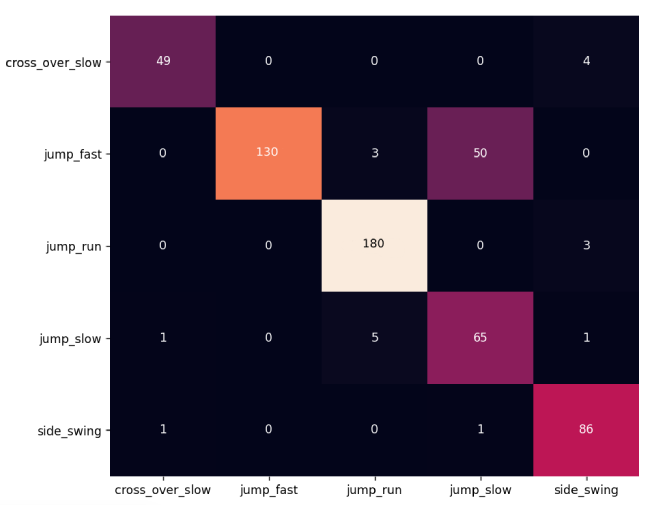
\includegraphics[width=0.5\textwidth]{rope_skipping/batchnormalization.PNG} 
  }
  \ffigbox[\FBwidth]{\caption{Individuele normalisatie}\label{fig:normalisation}}{%
    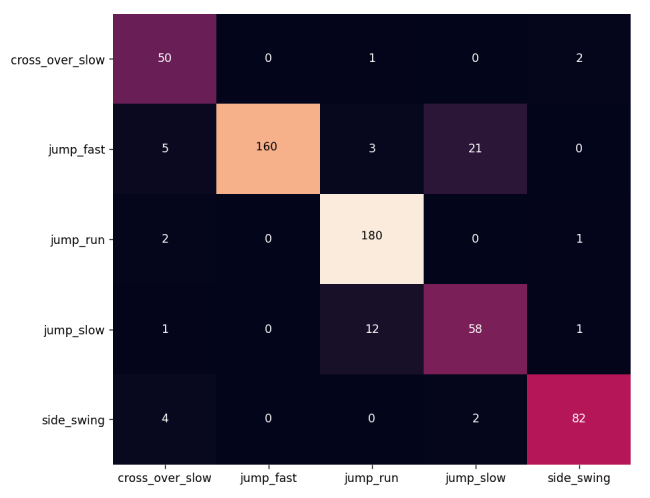
\includegraphics[width=0.5\textwidth]{rope_skipping/normalisatie.PNG}
  }
\end{floatrow}
\end{figure}

\subsubsection{Dropout}
Vervolgens volgt een Dropout laag. Deze laag moet overfitting voorkomen door een bepaald percentage van de input data te negeren. Er wordt gekozen om 30 procent van de datapunten buiten beschouwing te laten.

\subsubsection{MaxPooling1D}
De volgende laag is MaxPooling1D. Deze laag zal ervoor zorgen dat het aantal parameters gereduceerd wordt door telkens enkel de maximum vector te behouden binnen een gebied gedefinieerd door de pool\_size. Hier wordt gekozen voor een pool\_size van 2 en eveneens 2 strides. Dit wil zeggen dat de input gehalveerd zal worden aangezien de filter met grootte 2 telkens met twee eenheden verplaatst wordt.

\subsubsection{Flatten}
De volgende laag is Flatten en doet wat de naam zegt. Het zal de 3D input omvormen naar een 1D vector. Door deze laag toe te passen zal de uiteindelijke output van het model eveneens bestaan uit een 1D array in plaats van een meerdimensionale array.

\subsubsection{Dense/Fully connected}
Als laatste worden twee Dense lagen ingevoerd. De eerste Dense laag zal het dot product uitvoeren tussen de input matrix en de kernel met gewichten. De belangrijkste parameter hier is het aantal neuronen, wat de output shape vastlegt. De tweede dense laag heeft als activatie functie Softmax en zal zorgen voor de classificatie in de verschillende klassen.

\section{Berekeningen}
\subsection{Aantal draaiingen}
Het aantal draaiingen in een rope skipping sessie kan bekomen worden door naar de periode te kijken van het signaal. Deze periode is gelijk over x-, y- en z-as zoals te zien op Figuur \ref{fig:nofilter}. De side swing beweging is hierbij een uitzondering op de regel. De beweging vertoont een verschillend periodiek verloop langs de z-as (zie subsectie \ref{subsection:sideswing}). Eén periode langs deze as omvat een draaibeweging links en rechts van het lichaam. Deze periode wordt aanzien als één draaiing tijdens dit onderzoek. Bijgevolg zal in geval van de side swing beweging enkel rekening gehouden worden met de z-as.
Om het aantal periodes en dus het aantal draaiingen te berekenen, kan één periode manueel uitgesneden worden. Deze wordt dan geconvolueerd met het volledige signaal. De convolutie operatie zal grote pieken vertonen wanneer het signaal overeenkomt. Door deze pieken te tellen, is het aantal periodes en dus het aantal draaiingen geweten. Aangezien de periode voor verschillende sprongen uitgevoerd door verschillende proefpersonen niet telkens een gelijkaardig patroon zal vertonen, is deze manier niet toepasbaar.
Ook kan gekozen worden om de data in het 95\% kwartiel te bekijken. Elke periode heeft namelijk één uitgesproken piek, wat bijgevolg voor een hoge waarde zorgt. De amplitude van het signaal kan echter tijdens een sprong afzwakken of versterken zodat niet elke piek in het 95\% kwartiel voorkomt. Hierdoor is ook dit ook geen optimale methode.
Een laatste poging is om een Savitzky-Golayfilter op het signaal toe te passen. Deze filter zal binnen een vooraf gedefinieerd window een polynomiale functie proberen fitten \cite{ref70}. Een beter resultaat werd bekomen door met verschillende iteraties te werken in plaats van verhoging van het window. Tabel \ref{tab:filter} toont de gebruikte parameters per sprong.

Deze transformatie zal ervoor zorgen dat er per periode slechts één lokaal maxima aanwezig is. Door op dit geëffend signaal een piek detectie uit te voeren kan een vrij goede benadering gemaakt worden van het effectieve aantal draaiingen. Het gemiddelde wordt genomen tussen de drie assen omdat het signaal langs bepaalde assen soms een minder grote amplitude heeft wat kan resulteren in gewijzigde piekdetectie. Ook kan een extra piek, te wijten aan ruis langs een bepaalde as, zorgen voor te veel gedetecteerde draaiingen. Figuur \ref{fig:filter} geeft een gefilterd cross over signaal weer.

\begin{table}[!htpd]
  \centering
  \caption{Savitzky-Golayfilter parameters}
  \label{tab:filter}
\begin{tabular}{lccc}
 \hline \\
\textbf{}             & \textbf{Window} & \textbf{Poly-order } & \textbf{Iteraties} &  \\
\hline \\
\textbf{Jump run}     & 40               & 3            & 2        &  \\
\textbf{Jump slow}    & 50              & 3            & 1        &  \\
\textbf{Jump fast}    & 32               & 5            & 4        &  \\
\textbf{Cross over}   & 40               & 3               & 2        &  \\
\textbf{Side swing}   & 150                  & 5            & 2       & \\\\
\hline \\
\end{tabular}
\end{table}

\begin{figure}[!htpd]
\centering
\caption{Gefilterd signaal}\label{fig:filter}
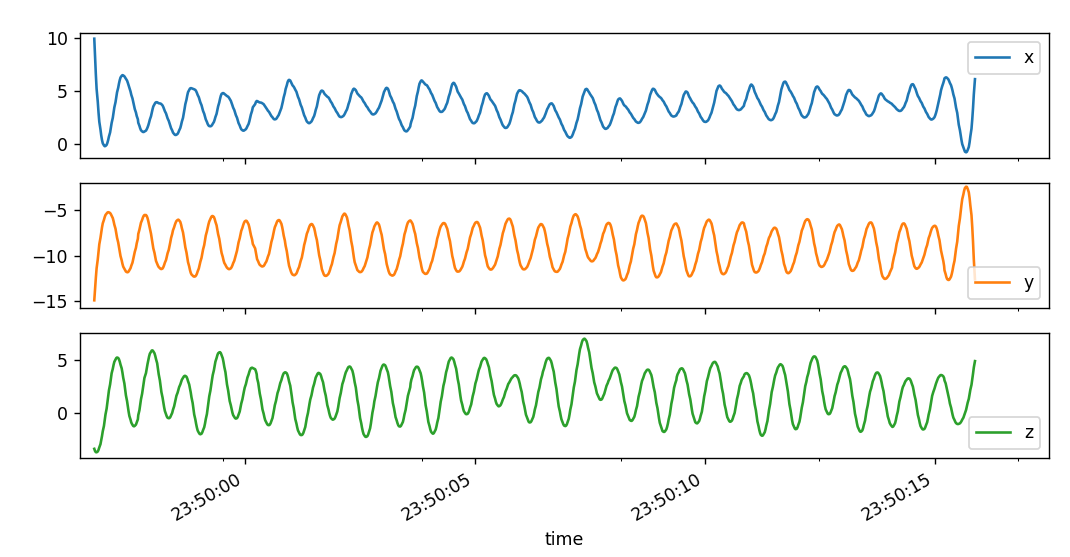
\includegraphics[width=.9\textwidth]{rope_skipping/crossover_gefilt.PNG} 
\end{figure}

\begin{figure}[!htpd]
\centering
\caption{Ongefilterd signaal}\label{fig:nofilter}
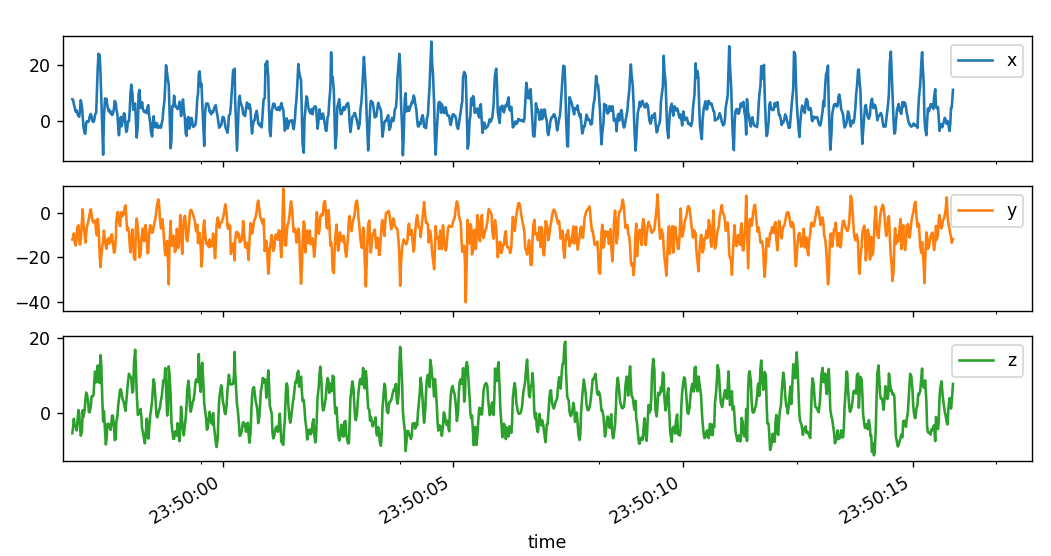
\includegraphics[width=.9\textwidth]{rope_skipping/crossover_nietgefilt.PNG} 
\end{figure}

\subsection{Fouten tijdens een beweging}
Wanneer een fout zich voordoet tijdens een sessie in de vorm van een hapering van het touw, dan is dit duidelijk merkbaar in het verloop van het signaal. Er zal voor enkele seconden geen of amper versnelling zichtbaar zijn. Dit is zichtbaar op Figuur \ref{fig:mistake} Door eerst de afgeleide te nemen van het signaal kan gefilterd worden op datapunten in een interval dichtbij 0. Indien een opeenvolgende reeks genoeg waarden bevat, wordt dit bestempeld als een fout. Via empirisch onderzoek werd deze parameter vastgelegd op 52 datapunten, wat ongeveer een halve seconde betekent. Het foutdetectie interval werd vastgelegd op een ondergrens van 10\% van de laagste en een bovengrens van 10\% van de hoogste piek. Tijdens de evaluatie bleek dat dit bij sprongen met een kleine amplitude een vertekend beeld kan geven vanwege de hogere amplitudes bij het starten met springen. Hierdoor werd gekozen voor een absoluut interval met ondergrens -0.000001 en bovengrens 0.000001.

\begin{figure}[!htpd]
\centering
\caption{Signaal met fout}\label{fig:mistake}
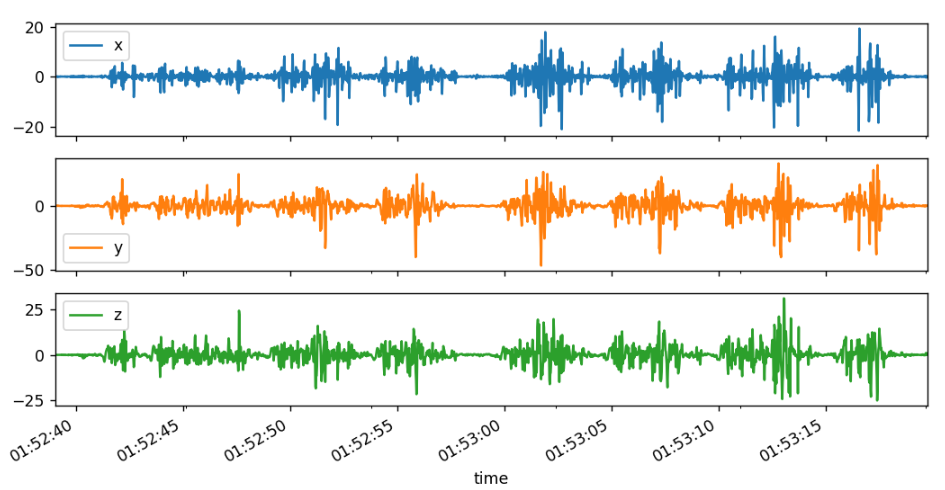
\includegraphics[width=.9\textwidth]{rope_skipping/mistake.PNG} 
\end{figure}

\chapter{Gezondheidsapplicatie}
Voorgaand onderzoek met betrekking tot herkenning van rope skipping bewegingen zal in wat volgt geïntegreerd worden in een gezondheidsapplicatie.
Met dit systeem is het de bedoeling dat de gebruiker via zijn/haar smartwatch sessies kan starten waarvan nadien statistieken weergegeven worden op de bijhorende smartphone applicatie. Hierbij wordt gefocust op rope skipping. Data processing van rope skipping zal gebeuren aan de hand van een eigen model (zie hoofdstuk \ref{chapter:3}). Een sessie rope skipping zal meer info geven aan de gebruiker in de vorm van tijdstippen met betrekking tot uitgevoerde bewegingen, het aantal draaiingen en eventuele geregistreerde tekortkomingen. Het is de bedoeling dat, gebaseerd op deze data, persoonlijke aanbevelingen gegeven worden. Alle informatie wordt, op basis van het id afkomstig van het Google account waarmee ingelogd werd, opgeslagen in een SQLite database. Dit gedeelte van het onderzoek werd uitgewerkt aan de hand van een voorgaande thesis \cite{ref73}. Hieruit werden ideeën opgedaan om vervolgens een eigen systeem te ontwikkelen.

\section{Backend - Frontend}
Het model werd getraind in Python. Er moet nu een afweging gemaakt worden tussen behouden van de scheiding van backend en frontend of migreren van de backend naar de frontend. Beide opties hebben voordelen en nadelen. Laten we eerst kijken naar de backend - frontend optie. Hierbij kan de code in Python behouden worden. Python is namelijk zeer efficiënt om aan data analyse te doen. Het beschikt over handige libraries zoals Pandas waarmee data door middel van reeds geïmplementeerde functionaliteit kan bewerkt worden. De server waarop de backend zou draaien heeft ook meer rekenkracht dan een android smartphone of smartwatch. Hierdoor kunnen zwaardere maar accuratere machine learning methodes gebruikt worden. Er is echter wel constant internetconnectie nodig om recente updates te krijgen.
Een louter frontend aanpak zal het probleem van offline werken aanpakken. De berekeningen worden nu op de applicatie zelf uitgevoerd. De resultaten zijn dus meteen beschikbaar voor de gebruiker. Een android smartphone heeft echter minder rekencapaciteit (alhoewel dit vandaag de dag nog meevalt) waardoor zeer zware berekeningen niet mogelijk zijn. Ook is het minder intuïtief om in Java aan data analyse te doen. 
Er werd gekozen voor de frontend aanpak. Dit omdat het belangrijk is meteen na een sessie statistieken weer te geven. Op die manier wordt voor optimale mentale stimulatie gezorgd. Zoals eerder vermeld, zijn hedendaagse android smartphones geschikt om zwaardere taken te draaien. Deze frontend aanpak is bijgevolg verantwoord. 

\section{Android opslag}
De applicatie zal aan de hand van vier Tensorflow Lite modellen online voorspellingen uitvoeren. Deze modellen moeten bijgevolg toegankelijk zijn voor de applicatie. Hierbij moet een keuze gemaakt worden tussen inwendig en uitwendig geheugen. Voor elke applicatie wordt bij opstarten een map voorzien in het inwendig geheugen. Hierin wordt gevoelige applicatie specifieke data opgeslagen en is bijgevolg niet toegankelijk voor andere applicaties. Het uitwendig geheugen daarentegen is toegankelijk voor elke applicatie. Ook is de beschikbare ruimte groter in vergelijking met het inwendig geheugen. Data opgeslagen in het uitwendig geheugen is echter minder betrouwbaar. De gebruiker kan namelijk elk moment beslissen om het geheugen te verwijderen \cite{ref75}. Om deze reden werd gekozen voor opslag in het inwendig geheugen.

\section{Smartwatch applicatie}
De smartwatch applicatie staat in voor het starten van sessies en het verzamelen van data tijdens deze sessies. De accelerometer en hartslag datapunten worden via de MessageClient API verstuurd naar de android applicatie draaiende op een smartphone. Aangezien aan een frequentie van 52Hz gemeten wordt, kan versturen van datapunten in realtime een invloed hebben op de batterijlevensduur en/of performantie van de applicatie. Om deze redenen wordt gekozen voor het verzenden van de data in batches van 104 datapunten. Voor de verzameling van hartslagdata moet de gebruiker eerst toestemming geven. De body sensors permissie wordt bestempeld als een zogenaamd gevaarlijke permissie waardoor deze \textit{at runtime} moet toegekend worden. 
De gebruiker wordt bij het starten van een sessie gevraagd om de corresponderende smartphone te selecteren. Indien deze niet in de lijst te vinden is, wordt gevraagd om bluetooth in te schakelen (zie Figuur \ref{fig:bluetooth}).
Tijdens een sessie wordt eveneens de hartslag gemonitord (zie Figuur \ref{fig:session}), indien deze gevaarlijk hoog wordt zal de smartwatch dit signaleren via een trilling. Hiervoor is extra informatie nodig. De maximum hartslag wordt namelijk berekend op basis van de leeftijd. Om deze reden zal, wanneer het startsignaal verstuurd wordt, een bericht met als inhoud de ingestelde leeftijd verkregen worden afkomstig van de smartphone applicatie.

\begin{figure}[!htpd]
\centering
\begin{floatrow}
  \ffigbox[\FBwidth]{\caption{Smartwatch session}\label{fig:session}}{%
    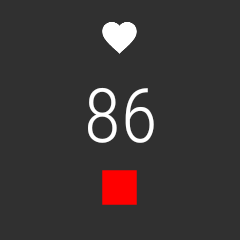
\includegraphics[width=.35\textwidth]{gezondheidsapplicatie/smartwatch-session.png}
  }
  \ffigbox[\FBwidth]{\caption{Smartwatch bluetooth}\label{fig:bluetooth}}{%
     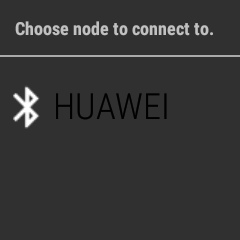
\includegraphics[width=.35\textwidth]{gezondheidsapplicatie/smartwatch-bluetooth.png}
  }
\end{floatrow}
\end{figure}

\section{Smartphone applicatie}
De smartphone applicatie staat in voor het ontvangen van datapunten en de verwerking hiervan. Het machine learning model is lokaal beschikbaar en wordt dan ook gebruikt om bewegingen te herkennen in de ontvangen accelerometer data. Ook worden het aantal draaiingen en eventuele fouten berekend. Per beweging zal het aantal MET-minuten (zie subsectie \ref{subsection:inspanningspunten}) berekend worden aan de hand van hartslag datapunten binnen een tijdsinterval bepaald door de duur van een sessie. Deze worden later gebruikt om aanbevelingen te genereren. 
Via een tijdlijn kan de gebruiker per sessie zien welke sprongen uitgevoerd werden (zie Figuur \ref{fig:tijdlijn}).
Elke week zullen de aanbevelingen berekend worden aan de hand van historische data. Deze zijn te zien op de applicatie zodat de gebruiker zelf kan kiezen wanneer hij/zij een aanbevolen activiteit uitvoert. Een aanbeveling kan omgezet worden in een effectieve sessie. Door een bericht te versturen via de MessageClient API naar de gekoppelde smartwatch wordt deze sessie gestart. De gebruiker wordt vervolgens gevraagd om de gewenste ontvanger te selecteren. Dit zodat geen problemen kunnen ondervonden worden indien meerdere bluetooth apparaten in de buurt aanwezig zijn (zie Figuur \ref{fig:bluetooth-phone}). De bijhorende aanbeveling wordt op \textit{pending} gezet zodat kan nagegaan worden of de gebruiker deze effectief uitvoert. Er wordt gecheckt of de duur van de activiteit overeenkomt met de aanbevolen duur en of het inspanningsniveau min of meer gelijklopend is.
Een afgewerkte aanbeveling wordt op \textit{done} gezet en uitgegrijsd weergegeven in de applicatie (zie Figuur \ref{fig:pending}).

\begin{figure}[!htpd]
\centering
\begin{floatrow}
  \ffigbox[\FBwidth]{\caption{Pending aanbevelingen}\label{fig:pending}}{%
    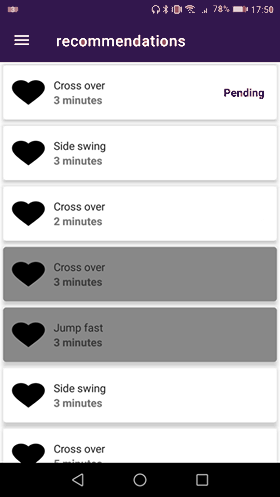
\includegraphics[width=.33\textwidth]{gezondheidsapplicatie/pending_recommendations.png} 
  }
  \ffigbox[\FBwidth]{\caption{Tijdlijn activiteiten}\label{fig:tijdlijn}}{%
    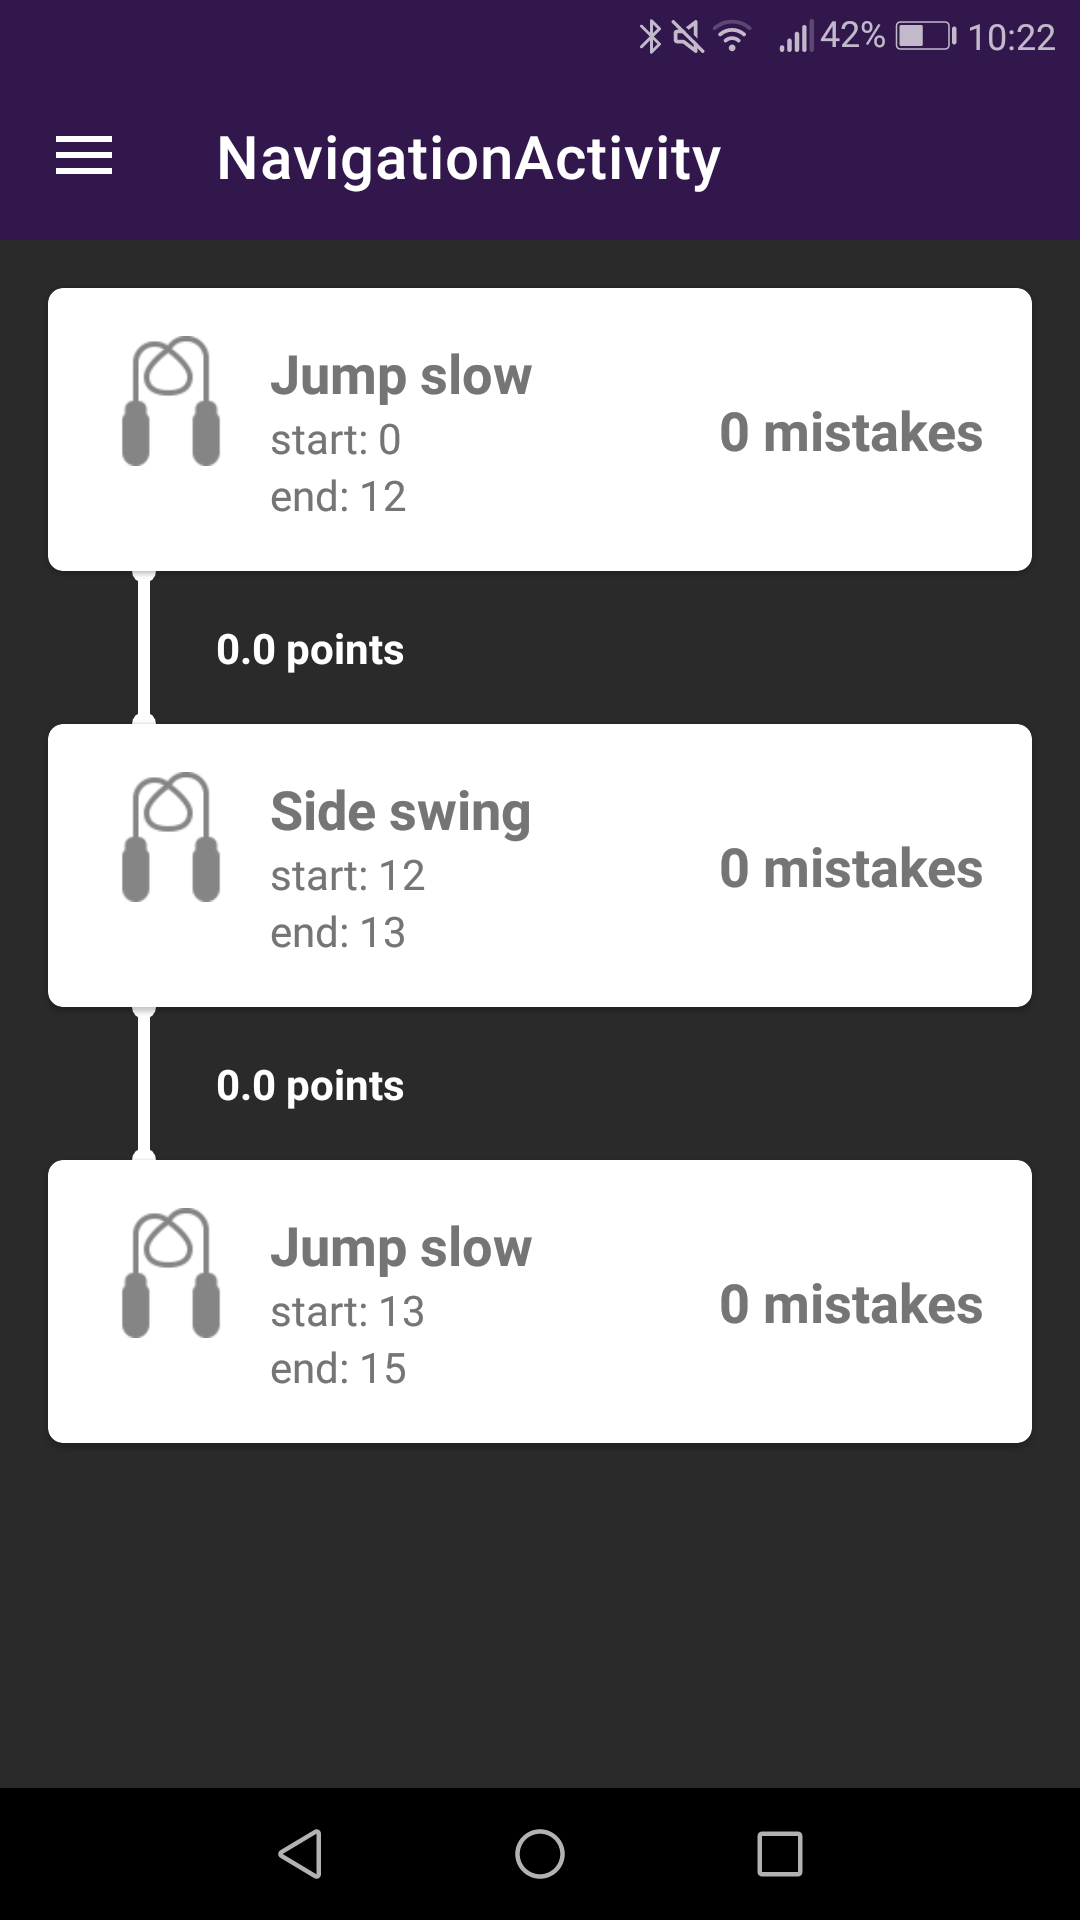
\includegraphics[width=.33\textwidth]{gezondheidsapplicatie/timeline.png} 
  }
  \ffigbox[\FBwidth]{\caption{Bluetooth dialog}\label{fig:bluetooth-phone}}{%
     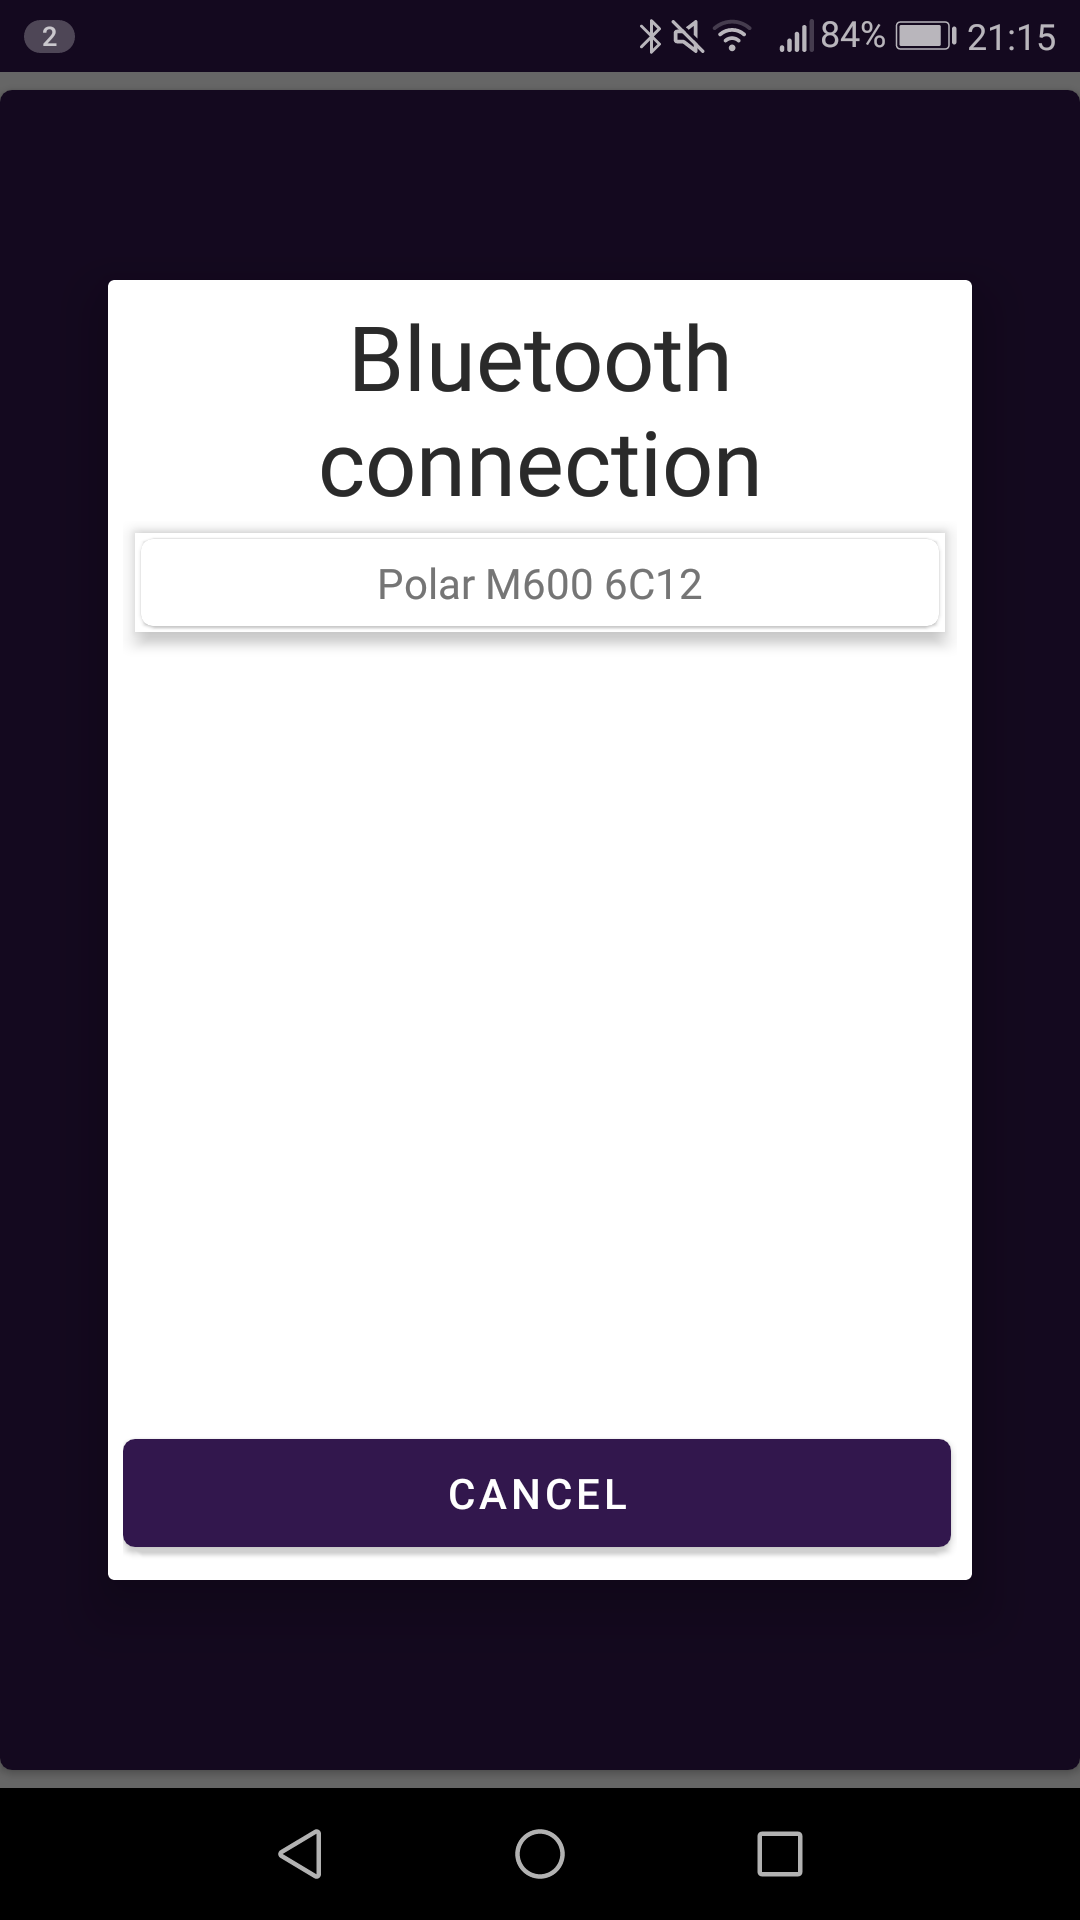
\includegraphics[width=.33\textwidth]{gezondheidsapplicatie/bluetooth_dialog.png} 
  }
\end{floatrow}
\end{figure}


\subsection{Aanbevelingen}
In deze subsectie worden eerst bestaande aanbevelingssystemen toegelicht. Vervolgens wordt het gebruikte aanbevelingsalgoritme besproken.

Een aanbevelingssysteem houdt rekening met de gebruiker en item dimensies.Er zijn verschillende manieren waarop dit kan geïmplementeerd worden.
Een eerste manier, Collaborative Filtering, bekijkt enkel interacties tussen gebruiker en item. Deze worden opgeslagen in een gebruiker-item interactie matrix. Verdere onderverdeling in een geheugen gebaseerde en een model gebaseerde aanpak is mogelijk. 

Een geheugen gebaseerde aanpak veronderstelt afwezigheid van een model en maakt in essentie gebruik van Nearest Neighbors. De items gekoppeld aan de gebruikers die het dichtst liggen worden aanbevolen. Ook hier kan nog eens een onderverdeling gemaakt worden in gebruiker-gebruiker en item-item.
Een gebruiker-gebruiker methode gaat gebruikers proberen identificeren met het meest gelijkaardige interactie profiel om zo nieuwe items aan te bevelen. Hierbij staat de gebruiker centraal. Gebruikers worden voorgesteld met een vector van hun interacties met items.
Een item-item methode gaat items zoeken gelijkaardig aan deze waarmee de gebruiker al positieve interactie mee had. Items worden gezien als gelijkaardig indien de twee gebruikers er op een gelijkaardige manier mee interageerden. Deze manier is bijgevolg gecentreerd rond het item.

Wanneer een model aanwezig is dan is er een zekere relatie tussen gebruiker en de gekoppelde items. Deze relatie wordt vervolgens gehanteerd bij voorspellingen.

Collaborative Filtering heeft als voordeel dat geen additionele info nodig is over gebruikers of items en kan dus in vele situaties gebuikt worden. Aanbevelingen worden ook accurater naarmate de gebruikers meer intrageren met items. Een nadeel is het cold start probleem. Dit doet zich voor door het feit dat enkel historische data bekeken wordt. Een nieuw item aanbevelen is onmogelijk en aan een nieuwe gebruiker kan niks aanbevolen worden. 

Content gebaseerde methoden gebruiken bijkomende info over de gebruiker en/of item objecten. Deze worden behandeld als features en kunnen helpen in verklaren waarom er juist een relatie is tussen die gebruiker en item. Deze methoden hebben geen last van cold start aangezien informatie altijd aanwezig zal zijn (leeftijd, geslacht..). Enkel nieuwe gebruikers of items met voorheen onbekende features ondervinden enige hinder.

Content gebaseerde methoden vervormen het probleem naar een classificatie of regressie probleem.
Indien de classificatie gebaseerd is op gebruikersfeatures dan wordt het item centraal geplaatst aangezien de berekeningen per item gebeuren.
Indien de classificatie echter op basis van item features wordt uitgevoerd dan is het algoritme gebruiker gecentreerd. Deze manier is persoonlijker omdat geen gebruik gemaakt wordt van data afkomstig van alle gebruikers. Het model is echter minder robuust vermits slechts één gebruiker met minder items interageerd \cite{ref50}.

Het systeem ontwikkeld tijdens deze thesis legt de nadruk vooral op het persoonlijke aspect. Daarom wordt gekozen voor een content gebaseerde methode gecentreerd rond de gebruiker. Het nadeel bij deze methode is hier ook niet echt van toepassing. Er zijn slechts een beperkt aantal bewegingen. De kans is dus groot dat 1 gebruiker deze allemaal uitvoert. Er zal echter wel enige hinder ondervonden worden door cold start. Van een nieuwe gebruiker is nog geen info geweten. Daarom worden een aantal willekeurige aanbevelingen gegenereerd zodat het systeem op termijn hieruit kan leren.

Elke week zal een nieuwe reeks aanbevelingen berekend worden. Hier wordt gebruik gemaakt van een PeriodicWorkRequest (zie subsectie \ref{subsection:workmanager}). Het ontwikkelde algoritme houdt rekening met het aantal sessies waarin een bepaalde activiteit uitgevoerd werd. Ook wordt het aantal fouten gemaakt tijdens een beweging in rekening gebracht. Er wordt gewerkt met een systeem dat gewichten toekent aan iedere activiteit op basis van eerder genoemde criteria. De duur van een aanbeveling wordt gelijkgesteld aan de gemiddelde duur van de gekozen activiteit op basis van historische data. Het totaal aantal MET-minuten van alle berekende aanbevelingen samen moet gelijk of groter zijn dan het doel gekoppeld aan die week. Dit totaal aantal METs wordt bekomen door gebruik te maken van het gemiddeld aantal METs per seconde voor iedere corresponderende activiteit en deze telkens op te tellen.
Indien nog geen sessies aanwezig zijn, dan kan nog geen rekening gehouden worden met de capaciteiten en voorkeuren van de gebruiker. Er wordt aan elke activiteit een gelijk gewicht toegekend. Om dezelfde reden wordt de duur van een activiteit willekeurig gekozen binnen het interval van 5 tot 10 minuten. Dit bleek een acceptabele duur te zijn voor beginnend rope skippers na enige rondvraging. Het is namelijk belangrijk om de initiële duur van de willekeurige aanbevelingen niet te groot te nemen. Een amateur rope skipper zou door een overschatting van zijn/haar capaciteiten al dan niet ontmoedigd worden. Het initiële doel wordt ingesteld op de gezonde waarde van 600 MET-minuten per week \cite{ref21}.
Een visualisatie van het ontwikkelde algoritme is te zien op Figuur \ref{fig:algo}.

\begin{figure}[!htpd]
\centering
\caption{Aanbevelingsalgoritme}\label{fig:algo}
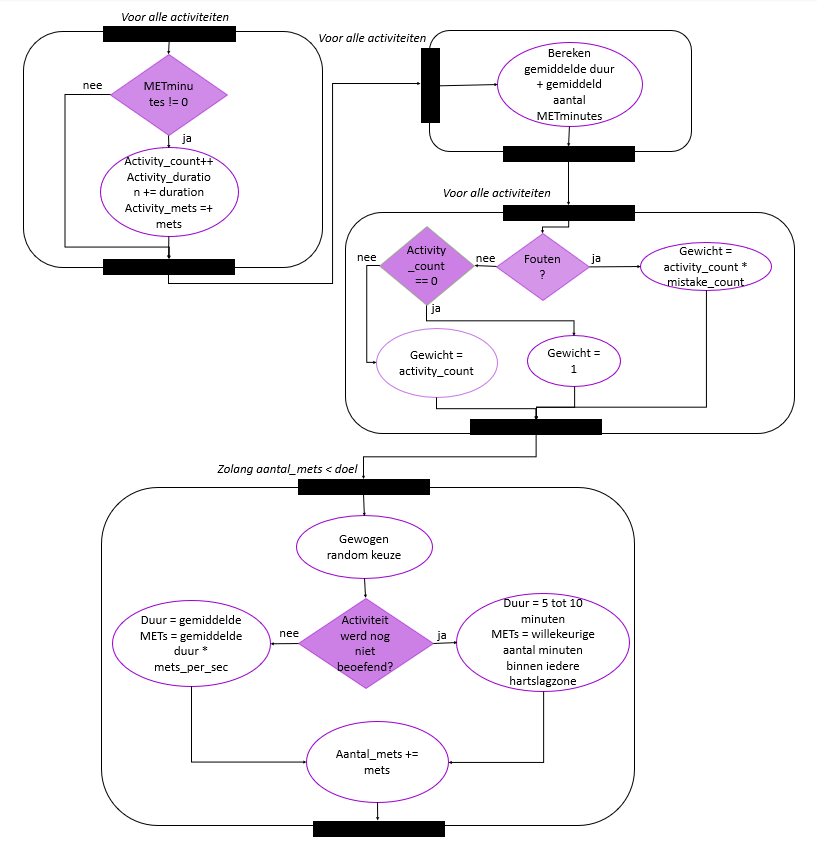
\includegraphics[width=1.15\textwidth]{gezondheidsapplicatie/recommendation_algo.PNG} 
\end{figure}

\subsection{Inspanningspunten} \label{subsection:inspanningspunten}
Het geven van persoonlijke aanbeveling steunt op een scoringmechanisme. De gebruikte metriek moet de mate van inspanning per activiteit correct weergeven. De MET-eenheid is hiervoor uitermate geschikt \cite{ref21}. Volgende paragrafen verduidelijken deze term.
De hoeveelheid energie die gebruikt wordt tijdens een inspanning is proportioneel tot de hoeveelheid zuurstof in het lichaam. Het aantal METs geeft hierbij de hoeveelheid zuurstof weer in geval van rust. De energie gevraagd van een fysieke activiteit kan uitgedrukt worden als een veelvoud van deze \textit{resting metabolic rate}. Dit is de Metabolic Equivalent of Task (MET). Een individu met gemiddelde fitness capaciteiten kan tot 12 METs verdragen, top atleten kunnen echter tot 20 aan. 
Een manier om het inspanningsniveau en dus het aantal METs te meten, is via de hoeveelheid zuurstof inname. Het zuurstofgehalte meten moet gebeuren aan de hand van strikte protocollen binnen een sport laboratorium. Dit is bijgevolg zeer tijdrovend en wordt dus enkel in speciale omstandigheden uitgevoerd. Door gebrek aan apparatuur en tijd wordt deze meetmanier in dit onderzoek niet gebruikt. 
Het is echter mogelijk om een relatieve benadering van de intensiteit te bekomen door de effecten op de hartslag en het respiratie gehalte te meten. 
De \textit{talk test} is hierbij één van de gebruikte methoden. Wanneer een persoon kan praten maar niet kan zingen, dan is de activiteit gemiddeld intensief. Wanneer de persoon ook niet meer kan praten dan is de activiteit \textit{vigorous intensief}. Gemiddeld en vigorous zijn klassen waarin de activiteit kan geclassificeerd worden op basis van de inspanning.
De \textit{heart rate test} gaat ervan uit dat de hartslag stijgt in een reguliere manier naarmate de intensiteit van de activiteit stijgt. De maximum hartslag kan berekend worden door de leeftijd af te trekken van 220 \cite{ref73}. 
De \textit{Submaximal excercise} test wordt gebruikt om de maximale fitness capaciteit te berekenen zonder hierbij boven de grens van 85\% van de maximale hartslag te stijgen. Door monitoring van de hartslag kan deze capaciteit geëxtrapoleerd worden met behulp van verschillende methoden. Deze waarde heeft echter gelimiteerde bruikbaarheid \cite{ref71}.

In het kader van dit onderzoek is de heart rate test het meest bruikbaar en wordt bijgevolg toegepast. Hierbij wordt het concept van hartslag zones gehanteerd.

Hartslag zones zijn een manier om te monitoren hoe hard getraind wordt. Het interval met als ondergrens de rusthartslag en als bovengrens de maximale hartslag op basis van leeftijd wordt gesplitst in 5 zones gebaseerd op de intensiteit van de training. Er zijn verschillende manieren om deze zones af te bakenen. Een veel gebruikte methode verwezenlijkt de afbakening aan de hand van percentages van de maximale hartslag. 

Volgende paragraaf licht de verschillende zones toe.
Hartslag zone 1 (50-60\% HRMAX) is de zeer lichte intensiteitszone. Trainen in deze zone zal de herstelling bevorderen en de sporter klaarstomen om te trainen in hogere zones. 
Hartslag zone 2 (60-70\% HRMAX) is de lichte intensiteitszone. Dit is de zone die het uithoudingsvermogen verbetert. Het lichaam wordt beter in oxideren van vet en de musculaire fitness zal samen met de capillaire densiteit stijgen. 
Hartslag zone 3 (70-80\% HRMAX) is de gemiddelde intensiteitszone. Deze zone bevordert de efficiëntie van de bloed circulatie in het hart en skelet spieren. Dit is de zone waar melkzuur begint te verbranden in de bloedstroom. 
Hartslag zone 4 (80-90\% HRMAX) is de harde intensiteitszone. In deze zone zal de ademhaling bemoeilijken en begint het anaerobic sporten. Dit betekent dat het lichaam zijn energie put uit bronnen naast zuurstof. In deze zone wordt het snelheidsuithoudingsvermogen getraind. Het lichaam wordt beter in het gebruik van carbohydraten voor energie. Hierbij zullen hogere levels van melkzuur in de bloedsomloop geconstateerd worden. 
Hartslag zone 5 (90-100\% HRMAX) is de maximum intensiteitszone. Melkzuur zal zich ophopen in de bloedsomloop. Dit is het niveau waarop atleten trainen \cite{ref72}.

Aan de hand van de tijd gespendeerd in bepaalde hartslag zones wordt een MET-score gekoppeld aan de activiteit (zie onderstaande formule). Dit geeft een accuraat beeld van hoe lastig deze was voor de gebruiker \cite{ref21}.
\[METminuten = 4*timeMPA + 8*timeVPA\]

\subsection{Doelberekening}
Het doel voor de volgende week wordt berekend door historische data tot tien weken in het verleden te bekijken. Deze data geeft weer hoeveel METs de gebruiker per week verbruikt heeft. Hiervan wordt het gemiddelde genomen. Dit zodat het doel niet te sterk stijgt of daalt en zo nog binnen de grenzen van mogelijkheden blijft. Wanneer niet genoeg data aanwezig is, wordt de historische data aangevuld met een waarde van 600 METs. Dit is volgens de literatuur het aan te raden MET verbruik per week \cite{ref21}.

\subsection{Authenticatie}
Aangezien bij onder andere de berekening van het aantal METs gebruik gemaakt wordt van persoonlijke gegevens, is authenticatie belangrijk. Ook de fitness data zelf is vertrouwelijk. Er wordt bijgevolg gebruik gemaakt van Google Sign In. Enkel bij inloggen is de lokaal opgeslagen data toegankelijk. Deze data is gelinkt aan een uniek userId bekomen vanuit Google Sign In. Op die manier is de vertrouwelijke data verbonden met de gebruiker en niet het fysieke toestel.
Voor het berekenen van MET-minuten per activiteit en per sessie moet de maximale hartslag geweten zijn. Deze wordt berekend aan de hand van volgende eenvoudige formule: 220 - leeftijd \cite{ref71} \cite{ref73}. Er zal dus gebruik gemaakt worden van de leeftijd van de gebruiker. De gebruiker zal bij inloggen zijn/haar leeftijd ingeven en zo de toestemming geven voor het gebruik en de opslag hiervan. 

\section{Evaluatie}
Om de evaluatie op een efficiënte manier tot een goed einde te brengen, worden enkele aanpassingen doorgevoerd. De aanbevelingen die gewoonlijk wekelijks berekend worden, zullen dagelijks gebeuren. Ook zal bijgevolg het doel dagelijks aangepast worden. De defaultwaarde hiervoor wordt ingesteld op afgerond 85 MET-minuten. Twee proefpersonen zullen gedurende enkele dagen gebruik maken van de ontworpen applicatie. Dit op zo'n manier zodat de uiteindelijke werkomstandigheden kunnen gesimuleerd worden. Elke dag zullen een aantal sessies uitvoeren waar de gezondheid en fitheid dit toelaat. Volgende secties zullen de waarnemingen en mogelijke werkpunten toelichten. Op die manier kan de applicatie optimaal functioneren in de praktijk.

\subsection{Werkpunten}
Na de eerste nieuwe doelberekening werd opgemerkt dat het doel niks veranderde ook al werd het eerste vooropgestelde doel niet gehaald. Dit kwam door de initiële keuze van een percentiel gerichte berekening. Hierbij zal er pas verandering komen in het doel na een aantal iteraties. Door deze observatie werd gekozen om over te schakelen op een gemiddelde berekening nog steeds met historische data van tien weken. 
Doordat de applicationContext vernietigd wordt bij het afsluiten van een applicatie zorgde dit voor problemen. Er werd namelijk gebruik gemaakt van deze context om het userId van de huidige gebruiker in bij te houden. Wanneer Workmanager op een moment dat de applicatie stand by is het nodige werk namelijk genereren van nieuwe aanbevelingen moet uitvoeren, was applicationContext niet beschikbaar. Dit is echter noodzakelijk om voor een bepaalde gebruiker de correcte data te verkrijgen. Dit probleem werd opgelost door een gebruiker eveneens op te slaan in de lokale databank. 
Om de fouten die het model nog maakt te compenseren werd gewerkt met gewichten. Tijdens het testen van de applicatie bleek namelijk dat detectie van jump fast moeilijk verliep. Daarom werd beslist om de probabiliteit van deze klasse telkens te vermenigvuldigen met een factor 1.5. Indien het model zeker is zal dit geen invloed hebben op de voorspelling. Wanneer getwijfeld wordt tussen jump fast en een andere klasse, dan zal jump fast echter de bovenhand nemen.

\subsection{Draaiingen}
Evaluatie van het aantal draaiingen en de geregistreerde fouten werd gedaan volgens een empirisch onderzoek. Hierbij werden de parameters telkens aangepast zodat de uitkomst dichter bij de werkelijkheid lag. Doordat de berekening van het aantal draaiingen afhankelijk is van de gedetecteerde klasse leidt dit tot een kleine verlaging in accuraatheid. Tabel \ref{tab:draaiingen} geeft het afgerond gemiddeld aantal draaiingen er te veel of te weinig gedetecteerd werden.

\subsection{Foutdetectie}
Vooraleer te beginnen met de beschrijving van de evaluatie wordt de gebruikte terminologie toegelicht. Valse positieven of \textit{false positives} zijn correcte bewegingen bestempeld als fout. \textit{True positives} stellen deze bewegingen voor die correct geclassificeerd werden als fout. Een \textit{false negative} doet zich voor wanneer een fout gemaakt werd, maar niet gedetecteerd.
Voor de gemaakte fouten werd eerst onderzocht hoelang deze gemiddeld duren. Er werd geconcludeerd dat de duur tussen stoppen met springen wegens een fout en terug herbeginnen ongeveer één seconde bedraagt. In eerste instantie werd gewerkt met een detectie interval afhankelijk van het signaal. Tijdens de evaluatie bleek echter dat dit voor minder goede detectie zorgde. In geval van bijvoorbeeld een sprong zoals jump fast waarbij de gemaakte bewegingen geen grote amplitude hebben, zullen veel valse positieven voorkomen. Dit omdat men bij de start van een sprong vaak een grotere beweging maakt om zo het touw een initiële versnelling te geven die groot genoeg is. Om deze reden werd ervoor gekozen het detectie interval onafhankelijk te maken van de sprong. Een interval met als ondergrens -0.0000001 en als bovengrens 0.0000001 bleek goede resultaten te leveren. Alhoewel er nog steeds een aantal valse positieven merkbaar zijn ten gevolge van jump fast. Dit overzicht is te zien in Tabel \ref{tab:fouten}. Figuur \ref{fig:evaluatie} toont een gedeeltelijk overzicht van de uitgevoerde evaluatie in de applicatie.

\begin{table}[!htpd]
\parbox{.45\linewidth}{
    \centering
    \begin{tabular}{lc}
 \hline \\
    \multicolumn{1}{c}{\textbf{}}          & \textbf{Foutenmarge} \\
     \hline \\
    \multicolumn{1}{c}{\textbf{Jump run}}  & 2                    \\
    \multicolumn{1}{c}{\textbf{Jump slow}} & 2                    \\
    \textbf{Jump fast}                     & 3                    \\
    \textbf{Side swing}                    & 1                    \\
    \textbf{Cross over}                    & 1   \\\\
     \hline \\
    \end{tabular}
    \caption{Detectie draaiingen}
    \label{tab:draaiingen}
}
\hfill
\parbox{.45\linewidth}{
    \centering
   \begin{tabular}{lc}
 \hline \\
    \textbf{}               & \textbf{Aantal} \\
     \hline \\
    \textbf{True positive}  & 11                \\
    \textbf{False positive} & 3                  \\
    \textbf{False negative}  & 2               \\\\
     \hline \\
    \end{tabular}
    \caption{Fout- en draaiingen detectie}
    \label{tab:fouten}
}
\end{table}

\begin{figure}[!htpd]
\centering
\caption{Evaluatie draaiing en foutdetectie}\label{fig:evaluatie}
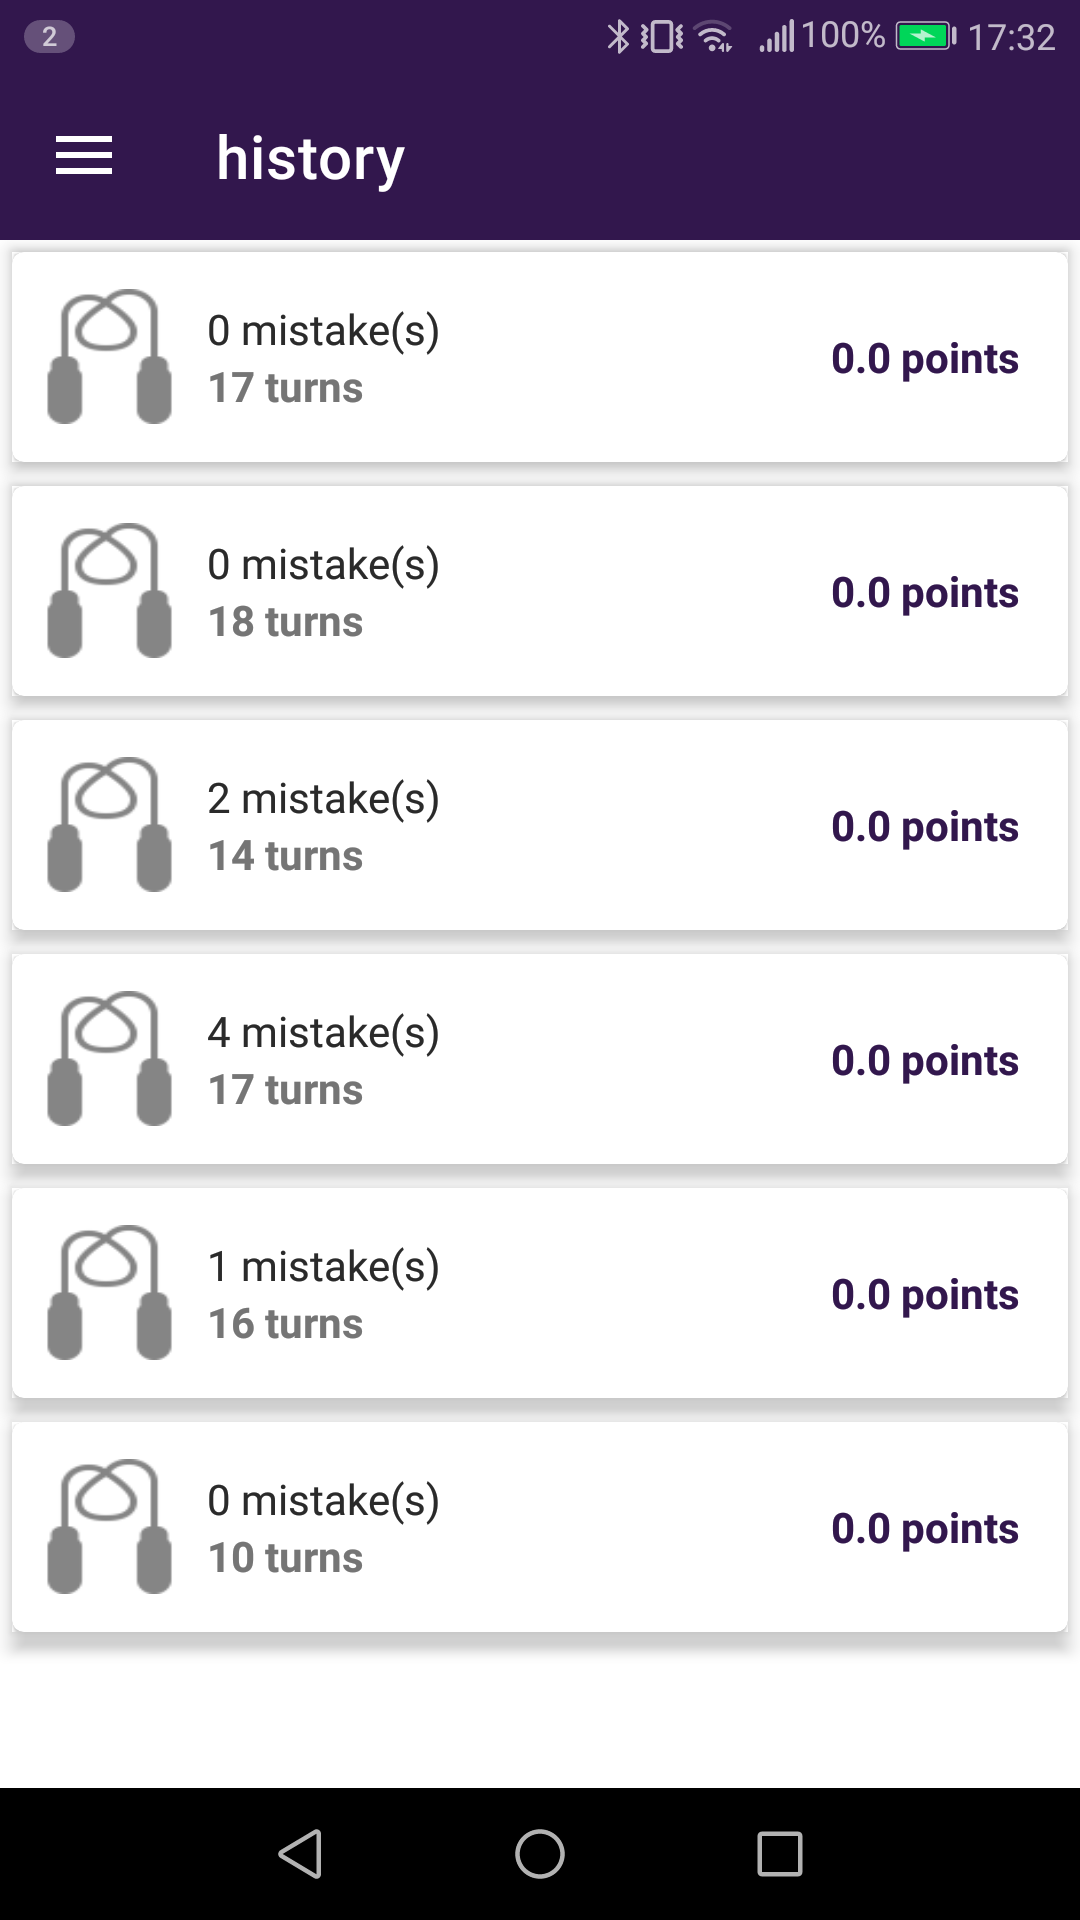
\includegraphics[width=0.45\textwidth]{gezondheidsapplicatie/history.png} 
\end{figure}

\subsection{Aanbevelingen}
Een eerste proefpersoon met gemiddelde fitheid evalueerde de applicatie gedurende drie dagen. Hierbij werd gefocust op de sprongen side swing en jump fast. Dit werd weerspiegeld in de gegeven aanbevelingen al na de eerste dag. Aangezien de sessies telkens van korte duur waren en hierbij minimale inspanning nodig was, werd het vooropgestelde doel niet gehaald. Dit weerspiegelde zich in het voorgestelde doel voor de volgende dag, wat 51 MET-minuten bedroeg. Dit patroon werd aangehouden gedurende twee additionele dagen. De aanbevelingen pasten zich aan aan de voorkeur van de gebruiker en de gewenste duur (zie Figuur \ref{fig:evaluatie1}).
Een tweede proefpersoon met slechtere conditie evalueerde de applicatie eveneens gedurende drie dagen. De gebruiker was enkel in staat om een side swing uit te voeren. Deze voorkeur weerspiegelde zicht duidelijk in de aanbevelingen (zie Figuur \ref{fig:evaluatie2}). Na de eerste dag zakte het doel met slechts 9 MET-minuten. Dit fenomeen zette zich verder de volgende dagen waarbij geëindigd werd met een doel van 60 MET-minuten. Dit is te verklaren door de hogere leeftijd van deze proefpersoon. Hierdoor wordt sneller een hoge hartslagzone bereikt.

\begin{figure}[!htpd]
\centering
\begin{floatrow}
  \ffigbox[\FBwidth]{\caption{Proefpersoon 1}\label{fig:evaluatie1}}{%
    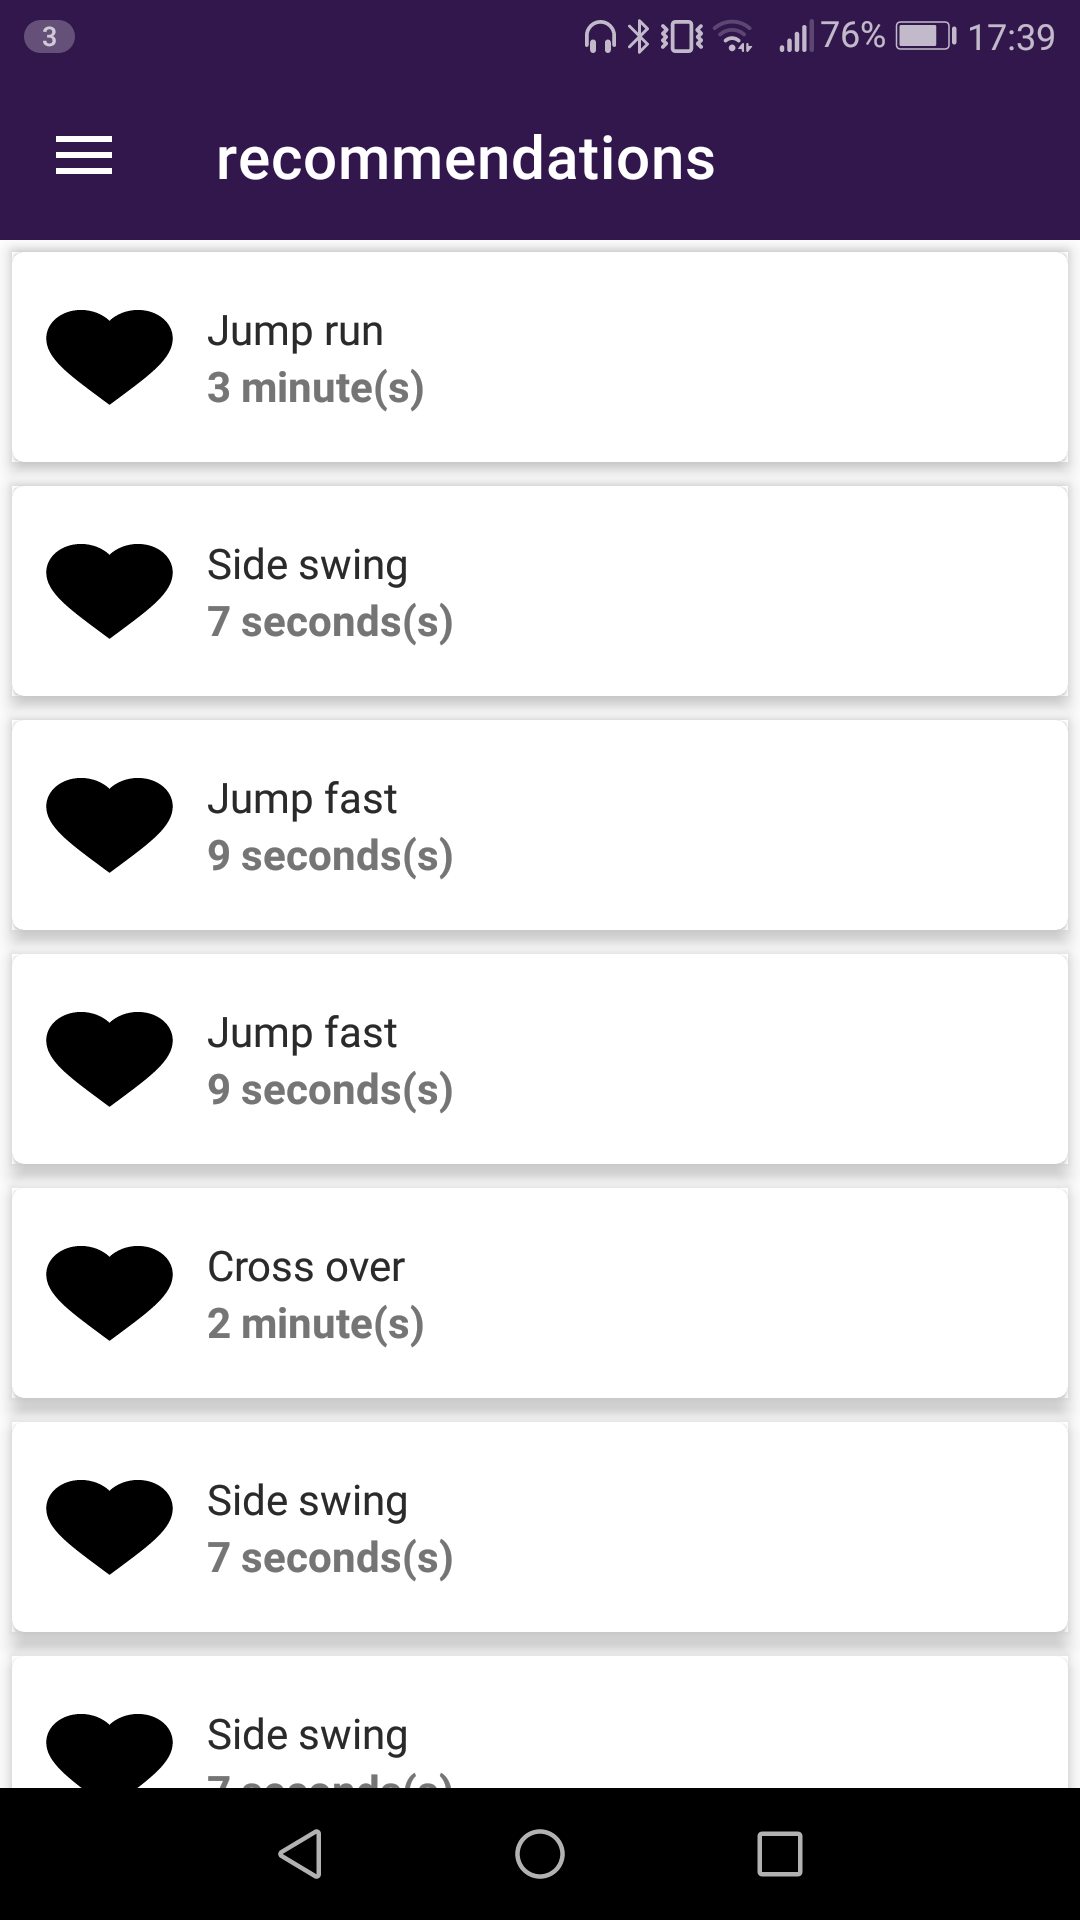
\includegraphics[width=0.45\textwidth]{gezondheidsapplicatie/proefpersoon1_recom.png} 
  }
  \ffigbox[\FBwidth]{\caption{Proefpersoon 2}\label{fig:evaluatie2}}{%
    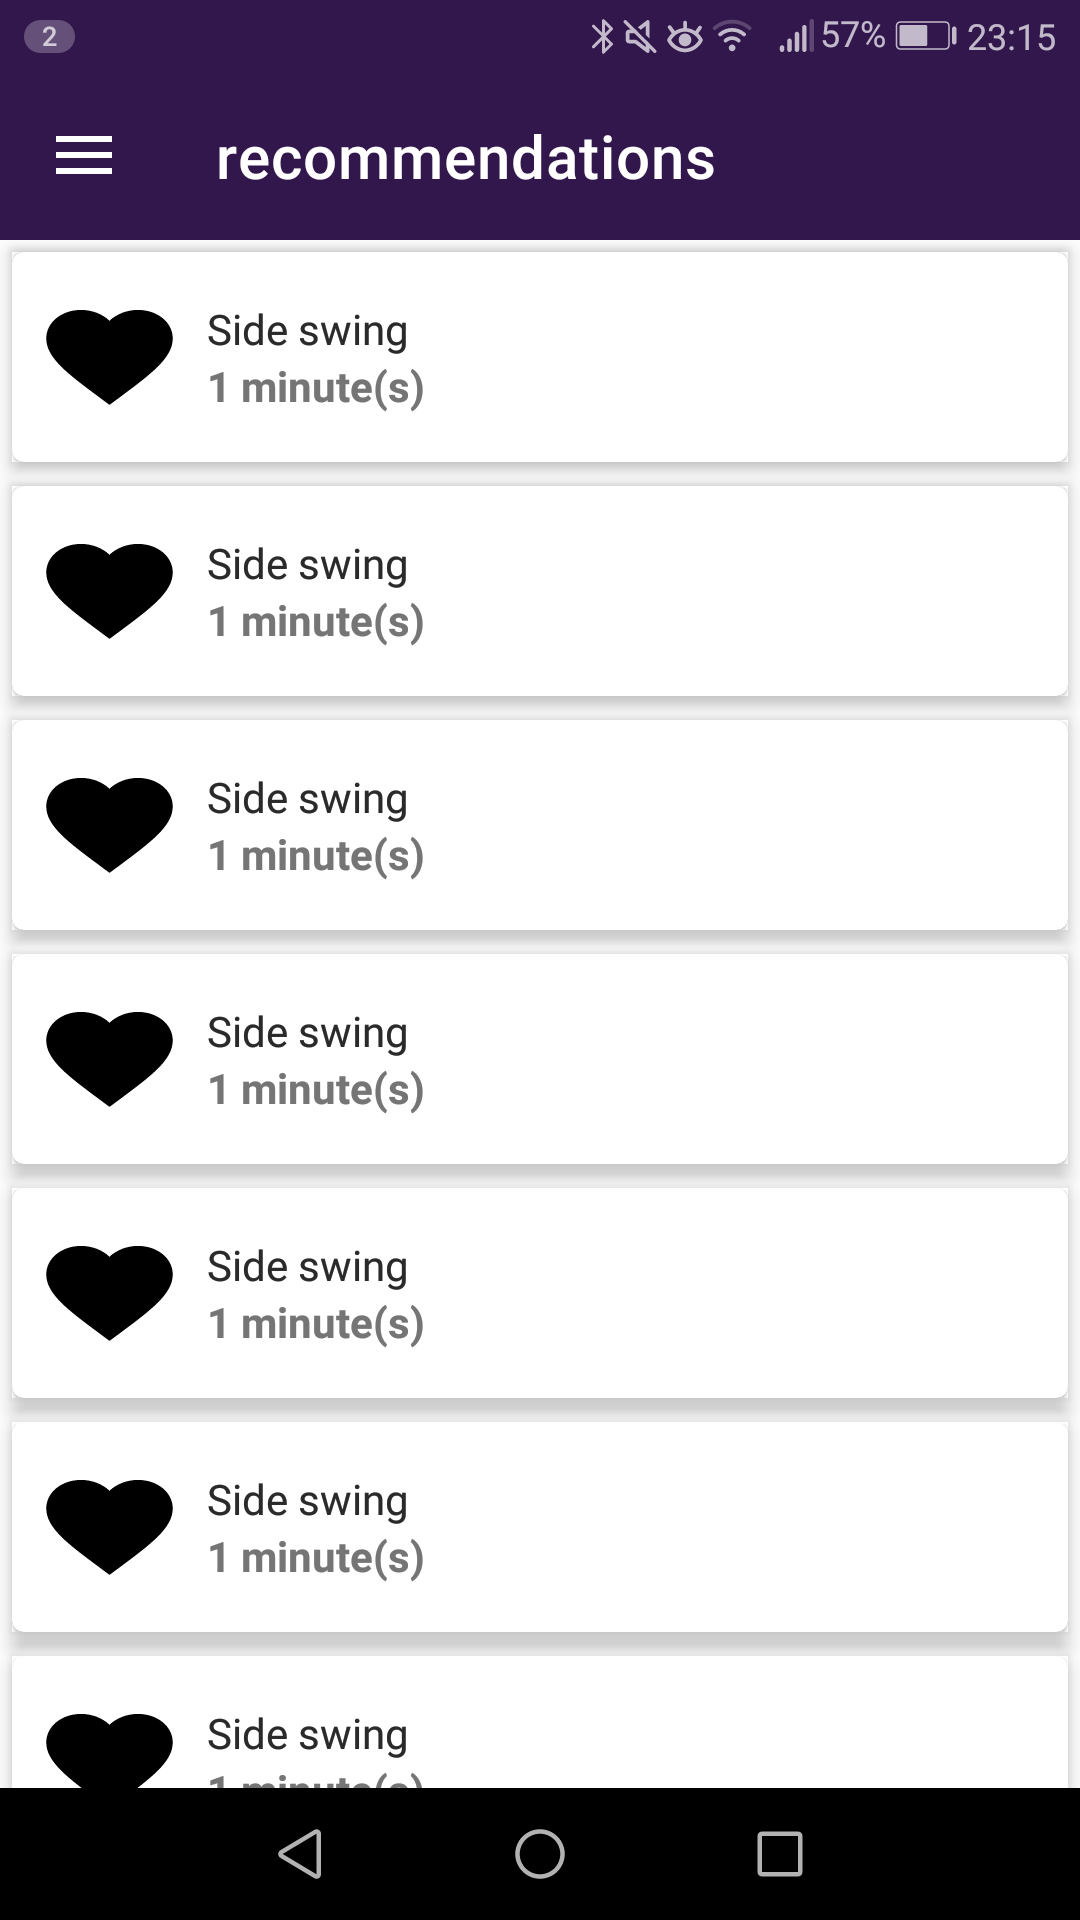
\includegraphics[width=0.45\textwidth]{gezondheidsapplicatie/proefpersoon2_recom.png}
  }
\end{floatrow}
\end{figure}

\chapter*{Conclusie}
Deze thesis onderzocht de mogelijkheden met betrekking tot herkenning van rope skipping bewegingen. Door gelimiteerde toegang tot verschillende sensoren konden enkel pols bewegingen onderzocht worden waardoor het aantal bewegingen gereduceerd werd. Variaties aangaande voetposities komen namelijk vaak voor binnen rope skipping.
Niettegenstaande werd bewezen dat verschillende bewegingen zich van elkaar onderscheiden louter met data afkomstig van polsbewegingen. In een eerste fase werd onderzocht welk machine learning algoritme het meest geschikt is voor dit classificatie probleem. Het convolutional neural network, afgekort CNN, gaf de beste resultaten. Vervolgens werd, toegepast op CNN, de meest optimale window grootte onderzocht. Hierbij werd gestart vanuit de hypothese dat een sprong gemiddeld één seconde duurt. Dit werd bevestigd tijdens het onderzoek. Windows van één seconde en meer bleken namelijk goede accuraatheden te leveren. Daaropvolgend werd nagegaan welke hoeveelheid overlapping zorgt voor de hoogste performantie. Hieruit bleek dat enige overlapping gunstig is. Overlappingen van 30, 50 en 70 procent resulteerden in gelijkaardige accuraatheden. Er werd geopteerd voor 30\% omwille van het risico op overfitting bij hogere percentages. 
Er werd eveneens nagegaan in welke mate variaties binnen een klasse resulteren in verlaging van de accuraatheid. Na splitsing werd een lichte stijging in accuraatheid vastgesteld bij de afzonderlijke modellen.
Als laatste experiment werd nagegaan welk effect ensemble learning heeft op de performantie. Hierbij werd geconstateerd dat meerdere samenwerkende modellen zorgen voor hogere accuraatheid.

Vervolgens werd dit model gebruikt binnen het kader van een gezondheidsapplicatie. Hierbij werd aangetoond dat aanbevelingen op basis van inspanningspunten en de persoonlijke voorkeur van de gebruiker kunnen geproduceerd worden. Via het weergeven van fouten en aantal draaiingen werd eveneens voor meer aanmoediging gezorgd. Op die manier ontstond een persoonlijk bewegingspatroon.

Door rekening te houden met de maximale hartslag gebaseerd op leeftijd kunnen te zware inspanningen gedetecteerd en gerapporteerd worden.

Er werd bijgevolg een antwoord geboden op de onderzoeksvragen aangehaald in de introductie.

Inzake toekomstig werk zijn er nog enkele mogelijkheden.
Vanwege de corona-maatregelen bleek het onmogelijk om voldoende proefpersonen te verkrijgen. Toekomstige studies kunnen het ontwikkelde model op deze manier nog verder generaliseren. Ook kan bij de gezondheidsapplicatie rekening gehouden worden met het stress-niveau en slaappatroon van de gebruiker. Op deze manier kunnen de aanbevelingen nog persoonlijker gemaakt worden. Ook kan nog meer rekening gehouden worden met gebruikerscontext inzake wekelijks patroon.

\bibliographystyle{unsrt}
\bibliography{references}
\afterpage{\blankpage}
\includepdf[page=-]{voorblad/titel} 
\end{document}
